\chapter{波函数和薛定谔方程}\label{chp:02} % Wave function and Schrödinger's equation
% \makebox[5em][s]{} % 短题目拉间距

量子力学的发展过程,错综复杂,我们不拟作详细的历史叙述,而将用尽量简明的逻辑,通过简单的对比分析,建立量子力学的基本方程—薛定谔方程,并围绕若薛定谔方程初步阐明波函数的含义然后讨论几种典型的一维定态问题.

第三章将全面地叙述量子力学的基本原理.
% 薛定谔方程
\input{QM file/body/C.two/M02.01-Schrödinger's equation}

% 波函数的统计诠释
\section[波函数的统计诠释]{波函数的统计诠释} \label{sec:02.02} % 
% \makebox[5em][s]{} % 短题目拉间距

薛定谔方程中的波函数中,$\varPsi$一般是复数,因此$\varPsi$不可能直接描述某种物理量,波函数的确切含义,在量子力学建立以后才弄明白.

还是从光子说起.用单色光做圆孔衍射实验,如图\ref{fig.2-1}所示.屏上出现的衍射图样(明暗相间的衍射环)是光具有波动性的确证.屏上各处(以及由孔至屏整个空间)衍射光的亮度和衍射波的强度(波函数的模方,即$|\varPsi|^{2}$)成正比.强度大处为亮环,强度小处为暗环.衍射图样的形状(亮环和暗环的位置)完全取决于光波波长$\lambda$及孔的半径以及孔至屏的距离,而和入射光的总强度无关.可见,衍射并非各个光子互相影响所造成,而是每个光子的运动规律,光的波动性体现在每个光子上.但就一个光子来说,衍射后它总只能出现在屏上某个地方,而不可能同时出现在几个地方.显然,一个光子在屏上某处出现的概率和该处衍射波的强度成正比.光波强度($|\varPsi|^{2}$)大的地方,到达的光子总数多,亮度大;光波强度小的地方,到达的光子总数少,亮度小.
\begin{figure}[!h]
	\centering
	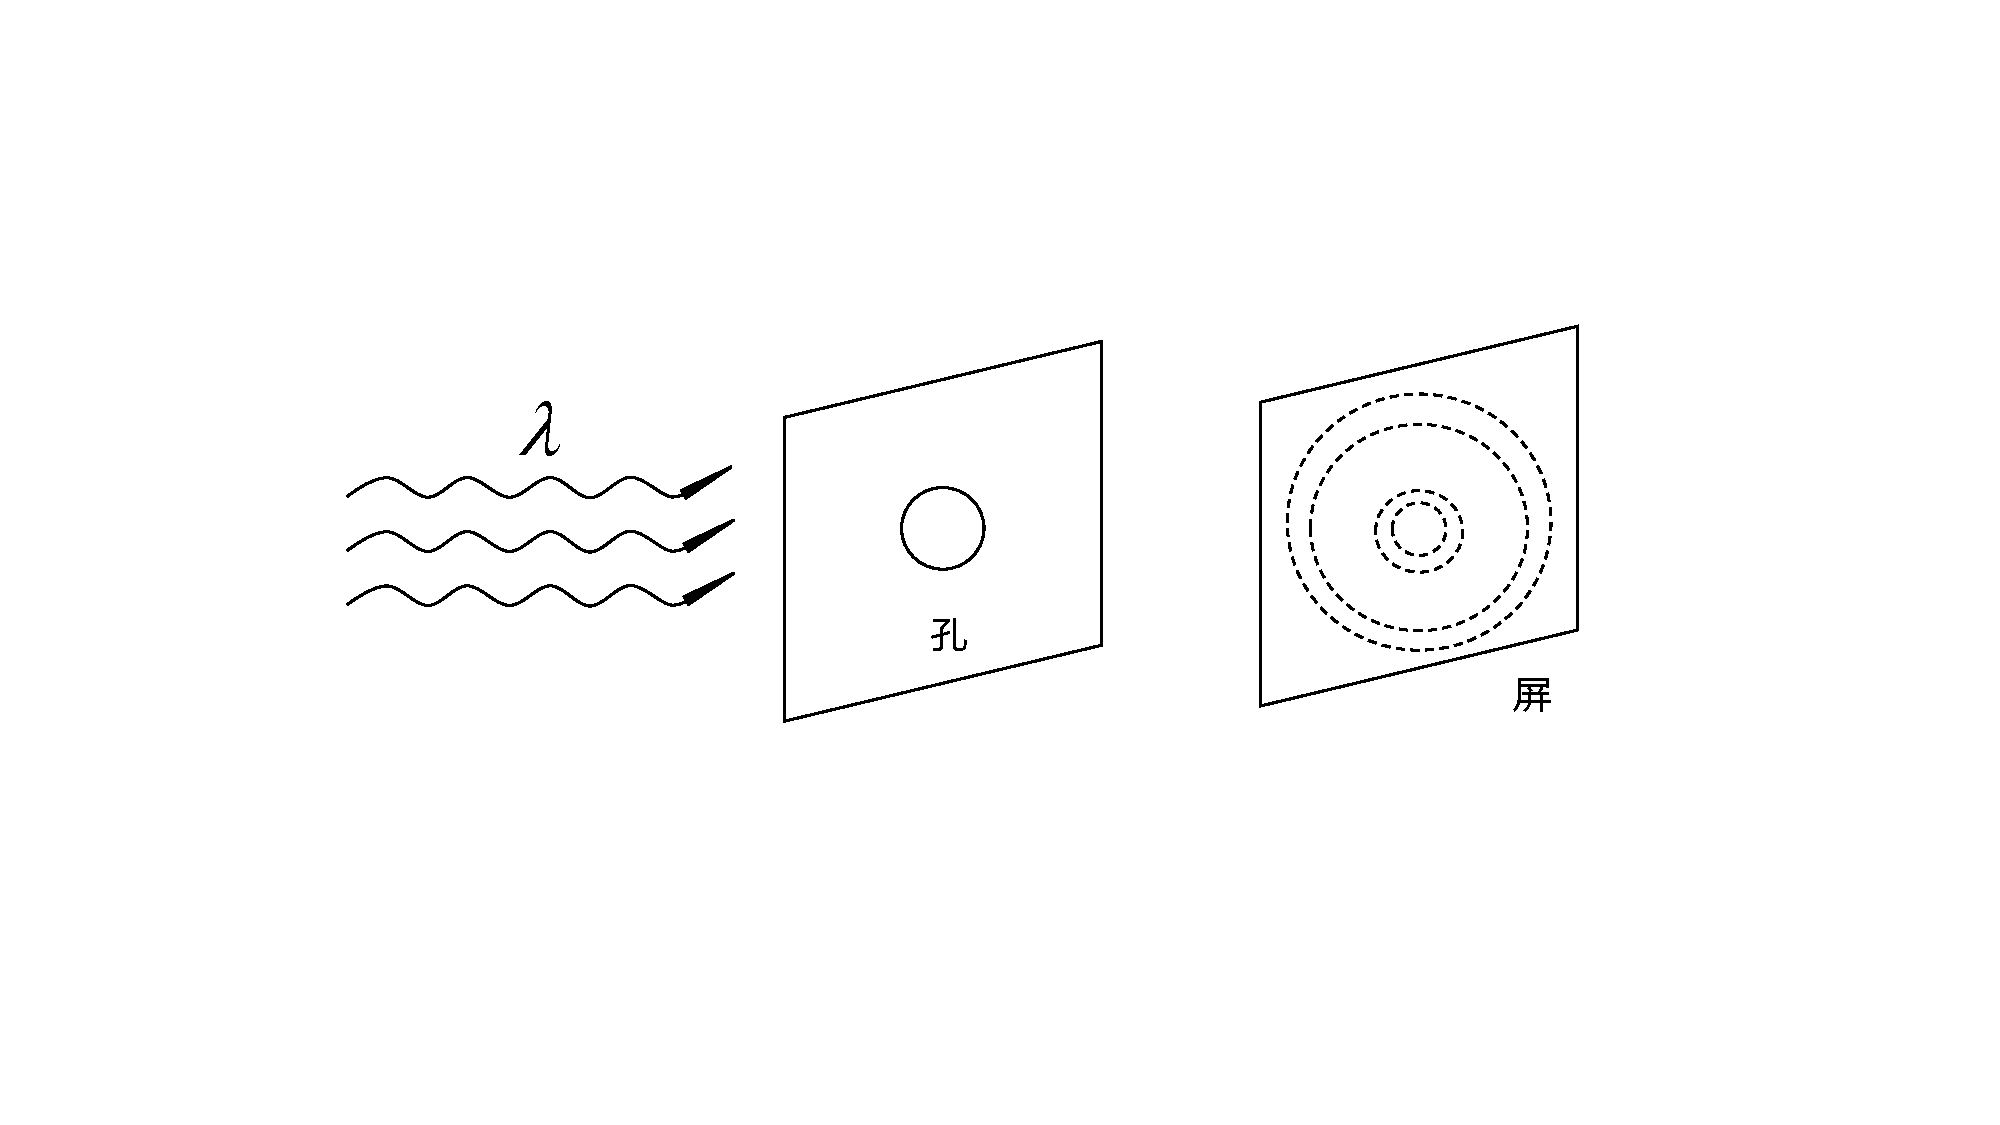
\includegraphics[width=5cm,clip]{QM file/figure/2-1}
	\caption{}\label{fig.2-1}
\end{figure}

用电子束代替光束进行的电子衍射实验结果类似,衍射图样取决于入射电子束的波长($\lambda=\frac{h}{p}$),而与电子总流量无关,这表明波动性是每一个电子的运动属性就一个电子来说,衍射后它将出现在屏上何处,事先无法预测,带有概率性;大量电子衍射的结果(相当于同样条件下单个电子衍射的多次重复),则表现出一定的规律性,屏上某处出现的电子总数和该处衍射波的(波函数的模方$|\varPsi|^{2}$)强度成正比.

基于这种认识,玻恩(M. Born)对薛定谔方程中的波函数提出了如下的统计诠释:
\eqlong
\begin{equation*}
	|\varPsi(\boldsymbol{r},t)|^{2} d\tau \propto \text{粒子在}t\text{时刻出现在}r\text{附近}d\tau\text{中的概率}
\end{equation*}
$d\tau=dxdydz$是$\boldsymbol{r}$附近的体积元.这个诠释被大多数物理学家接受.通常被认为是波函数的一项基本含义.($\varPsi$的更普遍的含义$\S$\ref{sec:03.04}将在讨论)玻恩对波函数的诠释带有基本假设的性质,它是不能用逻辑推理证明的,但巳为大章的实验事实(电子衍射实验就是其中之一)所证实.物质波因此也称“概率波”,$\varPsi$也称“概率波幅”.

概率性是微观物理现象的本质性特征,迄今人们掌握的微观基元过程,其物理规律的表现形式都带有概率性.以电子和原子的碰撞为例.用动量为$\boldsymbol{p}$$\bigg(\text{波长}\lambda=\frac{h}{p} \bigg)$的电子束撞击许多相同的处于基态的原子,碰撞是在电子、原子间一对一地进行.碰撞后有些原子仍处于基态,有些原子跃迁到激发态(设电子动量$\boldsymbol{p}$足够大,足以使原子激发)就一个原子来说,受电子碰撞后将跃迁到哪一个能级,事先是无法预测的,即碰撞结果带有概率性.但就大量原子来说,碰撞的结果(相当于电子、原子一对一碰撞的多次重复)处于基态和各激发态的原子数将有确定的相对比例,这些比例可以用量子力学计算出来.在这种意义上,可以说电子-原子碰撞是有规律的,这种规律具有概率性的特征.

回到$|\varPsi|^{2}$所表示的粒子空间概率分布问题.在低能范围,能量变化远小于粒子的静能$mc^{2}$,不涉及粒子的产生和湮没,粒子数应该守恒.就一个粒子的运动而言,任意时刻粒子在空间各处出现的总概率应该恒等于1 ,而且粒子总是出现在有限的空间区域内,这就要求$|\boldsymbol{r}|\rightarrow\infty$处波函数$\varPsi$迅速趋于0,以保证$|\varPsi|^{2}$的全空间积分
\begin{equation}\label{eq22.1}
	\int_{\text{全}} |\varPsi|^{2}d\tau=\iiint_{-\infty}^{\infty} |\varPsi|^{2}dxdydz=\text{有限值}
\end{equation}
在这条件下,显然
\begin{equation}\label{eq22.2}
	\text{粒子在}d\tau\text{中出现概率}=\frac{|\varPsi|^{2}d\tau}{\int_{\text{全}} |\varPsi|^{2}d\tau}
\end{equation}\eqshort

由于薛定谔方程是线性方程,如果函数$\varPsi_{1}(\boldsymbol{r},t)$是方程的解,则$\varPsi=A\varPsi_{1}$(A是任何常数)也是方程的解.这两个函数是描写同一种状态还是不同的状态?由波函数的统计诠释来看,按照\eqref{eq22.2}式,$\varPsi_{1}$和$\varPsi$所给出的粒子的空间概率分布并无不同,(第三章中将说明,状态的其他性质也并无不同.)因此应该认为$\varPsi_{1}$和$\varPsi=A\varPsi_{1}$描述同一种粒子状态.也就是说,给波函数乘上任何常数,并无任何新的物理意义.因此,对于满足平方可积条件\eqref{eq22.1}的波函数,总可以乘一个适当的系数,使之满足下列归一化条件:
\begin{equation}\label{eq22.3}
		\int_{\text{全}} |\varPsi|d\tau=1
\end{equation}\eqnormal
这样的波函数称为归一化的.这是\eqref{eq22.2}式简化为
\begin{equation*}\label{eq22.2'}
	\text{粒子在}d\tau\text{中出现概率}=|\varPsi|^{2}d\tau  \tag{$2.2.2^{\prime}$}
\end{equation*}\eqindent{5}
因此,$|\varPsi|^{2}=\varPsi^{*}\varPsi$称为粒子空间分布的“概率密度”.$\varPsi^{*}$表示$\varPsi$的共轭复数($\varPsi=u+iv,\varPsi^{*}=u-iv$).

为了讨论问题方便,有时也引入一些不满足平方可积条件\eqref{eq22.1}的波函数,它们相当于粒子的运动范围没有限制,粒子可以到达无限远处. 这时,$\varPsi$虽然不能归一化,但$|\varPsi|^{2}$仍具有相对概率的意义,即
\begin{equation}\label{eq22.4}
	\frac{\text{粒子在体积中}\tau_{1}\text{出现概率}}{\text{粒子在体积中}\tau_{2}\text{出现概率}}
	=\frac{\int_{\tau_{1}}|\varPsi|^{2}d\tau}{\int_{\tau_{2}}|\varPsi|^{2}d\tau}
\end{equation}\eqlong

电子具有电荷($-e$),当电子处于由波函数$\varPsi(\boldsymbol{r},t)$描述的某种运动状态时,如果在某个局部区域中电子出现概率为$\frac{1}{10}$,则从统计意义上说,该区域中具有电荷$\frac{-e}{10}$.这就是说,统计地看,电子的每一种运动状态(波函数$\varPsi$)相当于一种空间电荷分布,电荷密度为($-e$)$\varPsi^{*}\varPsi$.由于$\varPsi$是时间$t$的函数,$\varPsi^{*}\varPsi$可能随着$t$而变,则空间电荷分布也随$t$而变.按照电荷守恒定律,电荷分布的变化必然伴随着电流.由波函数$\varPsi$能否求出(统计意义下的)空间电流分布呢?这个问题涉及原子、分子等物质的电磁性质,其重要性是不言而喻的.薛定谔方程
\begin{equation}\label{eq22.5}
	i\hbar\frac{\partial}{\partial t}\varPsi
	=-\frac{\hbar^{2}}{2m}\nabla^{2}\varPsi+V(\boldsymbol{r})\varPsi
\end{equation}
可以回答这个问题.以$\varPsi^{*}$从左边乘上式各项,得到
\begin{equation*}
	i\hbar\varPsi^{*}\frac{\partial}{\partial t}\varPsi
	=-\frac{\hbar^{2}}{2m}\varPsi^{*}\nabla^{2}\varPsi+\varPsi^{*}V\varPsi
\end{equation*}
取复共轭,得到(注意$V^{*}=V$)
\begin{equation*}
	-i\hbar\varPsi\frac{\partial}{\partial t}\varPsi^{*}
	=-\frac{\hbar^{2}}{2m}\varPsi\nabla^{2}\varPsi^{*}+\varPsi V\varPsi^{*}
\end{equation*}
二式相减,得到
\begin{equation}
	\begin{aligned} \notag
		i\hbar\frac{\partial}{\partial t}(\varPsi^{*}\varPsi)
		&=-\frac{\hbar^{2}}{2m}(\varPsi^{*}\nabla^{2}\varPsi-\varPsi\nabla^{2}\varPsi^{*}) \\
		&=-\frac{\hbar^{2}}{2m}\nabla\cdot(\varPsi^{*}\nabla\varPsi-\varPsi\nabla\varPsi^{*})
	\end{aligned}
\end{equation}
亦即
\begin{equation}\label{eq22.6}
	\frac{\partial}{\partial t}(\varPsi^{*}\varPsi)+\nabla\cdot
	\big[-\frac{i\hbar}{2m} (\varPsi^{*}\nabla\varPsi-\varPsi\nabla\varPsi^{*}) \big]=0
\end{equation}\eqshort
这公式和经典物理中的连续性方程结构类似.流体力学中反映流体质量守恒的连续性方程是
\begin{equation}\label{eq22.7}
	\frac{\partial \rho}{\partial t}+\nabla\cdot(\rho v)=0
\end{equation}
$\rho$是流体的质量密度,$\boldsymbol{v}$是速度,$\rho\boldsymbol{v}$是流量密度(单位时间内在单位横截面积上流过的流体质量).电磁学中反映电荷守恒定律的连续性方程也取\eqref{eq22.7}式的结构,$\rho$是电荷密度,$\boldsymbol{v}$为电荷的运动速度, $\boldsymbol{j}=\rho\boldsymbol{v}$是电流密度.\eqref{eq22.6}式是量子力学中的连续性方程,它是粒子的空间分布概率守恒定律的表现形式.\eqref{eq22.6}式可以写成
\begin{equation*} \label{eq22.6'}
	\frac{\partial}{\partial t}\rho+\nabla\cdot\boldsymbol{j}=0 \tag{$2.2.6^{\prime}$}
\end{equation*}
其中
\begin{equation}\label{eq22.8}
	\rho=\varPsi^{*}\varPsi
\end{equation}\eqnormal
\begin{equation} \label{eq22.9}
	\begin{aligned}
		\boldsymbol{j}
			&=-\frac{i\hbar}{2m}(\varPsi^{*}\nabla\varPsi-\varPsi\nabla\varPsi^{*}) \\
			&=\frac{1}{2}(\varPsi^{*}\hat{\boldsymbol{p}}\varPsi+c.c^{\ddag}.) \\
			&=\Re\bigg(\varPsi^{*}\frac{\hat{\boldsymbol{p}}}{m}\varPsi \bigg)
			 =\Re(\varPsi^{*}\hat{\boldsymbol{v}}\varPsi)
	\end{aligned}
\end{equation}
\blfootnote{$\ddag$ 表示某项之复共轭,即将虚数单位i前正负号相反后的项.\qquad ——编注}
$\rho$称为“概率密度”,$j$称为“概率流密度”.$j$的最后表示式中,$\Re$表示取复数的实部,$\hat{\boldsymbol{v}}=\frac{\hat{\boldsymbol{p}}}{m}$是粒子的速度算符.

利用数学中的高斯(Gauss)定理
\begin{equation*}
	\iiint_{\tau}\nabla\cdot \boldsymbol{j}d\tau
	=-\iint_{S}j\cdot d\boldsymbol{S}=\iint_{S}j_{n}dS
\end{equation*}\eqindent{5}
($S$是体积$\tau$的表面,$d\boldsymbol{S}$是$S$的面元,$\boldsymbol{n}$是$d\boldsymbol{S}$的外向法线.)

将\eqref{eq22.6}式在任意体积$\tau$内积分,得到
\begin{equation} \label{eq22.10}
	\begin{aligned}
		\frac{\partial}{\partial t}\iiint_{\tau}\varPsi^{*}\varPsi d\tau
		&=-\iiint_{\tau}\nabla\cdot\boldsymbol{j}d\tau=-\iint_{S}\boldsymbol{j}\cdot d\boldsymbol{S} \\
		&=\frac{i\hbar}{2m}\iint_{S}(\varPsi^{*}\nabla\varPsi-\varPsi\nabla\varPsi^{*})\cdot d\boldsymbol{S}
	\end{aligned}
\end{equation}\eqshort
上式的意义是,体积$\tau$内概率的增率等于概率的流入率. 当将积分区域扩展到全空间, 如在无限远处$\varPsi$迅速趋于0,以保证\eqref{eq22.10}式中的面积分趋于0,就得到
\begin{equation}\label{eq22.11}
	\frac{\partial}{\partial t}\iiint_{\text{全}}\varPsi^{*}\varPsi d\tau=0
\end{equation}\eqnormal
即总概率守恒.由此可见,薛定谔方程\eqref{eq22.5}能够保证粒子空间分布的总概率守恒,亦即粒子数守恒.电磁波的波动方程[\ref{eq21.1}式]就没有这种性质,光子数是不守恒的.

对于电子(电荷$q=-e$),处于$\varPsi$描述的状态中时,统计意义下的电荷密度和电荷密度为
\begin{equation}\label{eq22.12}
	\rho_{c}=q\varPsi^{*}\varPsi=(-e)\varPsi^{*}\varPsi
\end{equation}
\begin{equation}
	\begin{aligned} \label{eq22.13}
		\boldsymbol{j}_{e}
		&=-\frac{i\hbar}{2m}q(\varPsi^{*}\nabla\varPsi-\varPsi\nabla\varPsi^{*}) \\
		&=(-e)Re\bigg(\varPsi^{*}\frac{\hat{\boldsymbol{p}}}{m}\varPsi \bigg)
		 =(-e)Re(\varPsi^{*}\hat{\boldsymbol{v}}\varPsi)
	\end{aligned}
\end{equation}\eqshort
注意电流密度与电荷密度的量子力学关系和经典电磁学关系有点相似,后者为$\boldsymbol{j}=\rho\boldsymbol{v}$,而在量子力学公式\eqref{eq22.13}中,表示粒子速度的算符:
\begin{equation}\label{eq22.14}
	\hat{\boldsymbol{v}}=\frac{\hat{\boldsymbol{p}}}{m}=-\frac{i\hbar}{m}\nabla
\end{equation}\eqnormal
必须放在$\varPsi^{*}$和$\varPsi$之间,即$\hat{\boldsymbol{v}}$仅作用于$\varPsi$.注意$\varPsi^{*}\hat{\boldsymbol{v}}\varPsi\neq\hat{v}\varPsi^{*}\varPsi$.

最后,讨论一下$\varPsi$波函数在无限远处的渐近性质.

在一维问题($-\infty < x < \infty$)中,$\varPsi$的归一化条件为
\begin{equation}\label{eq22.15}
	\int_{-\infty}^{\infty}\varPsi^{*}\varPsi dx=1
\end{equation}
$x\rightarrow\pm\infty$,显然$\varPsi$必须比$x^{-\frac{1}{2}}$更快地趋于0,才能满足归一化条件.

在三维问题中,如采用球坐标$(r,\theta,\varphi)$,体积元为
\begin{equation*}
	d\tau=r^{2}dr\sin\theta d\theta d\varphi
\end{equation*}\eqindent{5}
波函数的归一化条件为
\begin{equation}\label{eq22.16}
	\int_{\text{全}}\varPsi^{*}\varPsi d\tau=\int_{0}^{2\pi}d\varphi\int_{0}^{\pi}\sin\theta d\theta\int_{0}^{\infty}\varPsi^{*}\varPsi r^{2}dr
\end{equation}\eqshort
当$r\rightarrow\infty$,显然$\varPsi$必须比$r^{-\frac{3}{2}}$更快地趋于0,才能满足归一化条件.而为了保证总概率守恒,需要在$r\rightarrow\infty$的大球面上,\eqref{eq22.10}式右端的面积分趋于0,条件显然是
\begin{equation*}
	r\varPsi^{*}\varPsi\stackrel{r\rightarrow\infty}{\longrightarrow}0
\end{equation*}\eqnormal
即$\varPsi$必须比$r^{-\frac{1}{2}}$更快地趋于0.当$\varPsi$满足归一化条件时,称为束缚态.

\example 平面波的$\rho$和$\boldsymbol{j}$

\solution 具有确定能量$(E=\hbar\omega)$和动量$(\boldsymbol{p}=\hbar\boldsymbol{k})$的自由粒子,波函数为
\begin{equation}\label{eq22.17}
	\varPsi_{k}(\boldsymbol{r},t)=Ae^{i(\boldsymbol{k}\cdot r-\omega t)},\quad \omega=\frac{\hbar k^{2}}{2m}
\end{equation}
它是\eqref{eq21.11}式的定态特解,习惯上称为自由粒子平面波,$A$为“振幅”.按照\eqref{eq22.8}式,概率密度为
\begin{equation}\label{eq22.18}
	\rho=\varPsi_{k}^{\prime\prime}\varPsi_{k}=|A|^{2}
\end{equation}
$\rho$为常量,与$\boldsymbol{r},t$无关,这反映下列事实:当粒子处于$\varPsi_{k}$状态时,在空间各处出现的概率相同.按照\eqref{eq22.9}式,概率流密度为
\begin{equation}\label{eq22.19}
	\boldsymbol{j}=|A|^{2}\frac{\hbar \boldsymbol{k}}{m}=\frac{\rho\boldsymbol{p}}{m}=\rho v
\end{equation}
$\boldsymbol{v}=\frac{\hbar \boldsymbol{k}}{m}$为粒子的运动速度.注意\eqref{eq22.19}式和经典$\rho-\boldsymbol{j}$关系相似.\eqref{eq22.17}式可以描写具有确定动量的分布均匀的粒子束的流动,如单位体积中粒子数为$N$,取$A=\sqrt{N}$,则
\begin{equation*}
	\rho=N,\quad \boldsymbol{j}=N\boldsymbol{v}
\end{equation*}
$\boldsymbol{j}$表示沿速度方向单位横截面积上单位时间内通过的粒子数,即粒子数流量.

注意,平面波\eqref{eq22.17}式不是平方可积的,不能归一化,这是一种游离态,粒子可以在无限远处出现.









% 定态
\section[定态]{\makebox[5em][s]{定态}} \label{sec:02.03} % 
% \makebox[5em][s]{} % 短题目拉间距

本节讨论定态波函数的一般数学性质,而以一维束缚定态作为讨论的重点.

在$\S$\ref{sec:02.01}中已经讲过,具有确定能量值的状态称为定态,定态波函数的时空变量可以分离,一般形式为
\begin{equation}\label{eq23.1}
	\varPsi_{E}(\boldsymbol{r},t)=\varPsi_{E}(\boldsymbol{r})e^{-iEt/\hbar}
\end{equation}
其中$\varPsi_{E}(\boldsymbol{r})$满足定态薛定谔方程:
\begin{equation}\label{eq23.2}
	\hat{H}\varPsi(\boldsymbol{r})=E\varPsi(r)
\end{equation}
本节只讨论哈密顿量$H$等于动能加势能的情形,即
\begin{equation}\label{eq23.3}
	\hat{H}=\hat{T}+V=-\frac{\hbar^{2}}{2m}\nabla^{2}+V(r)
\end{equation}
这时定态薛定谔方程为
\begin{equation}\label{eq23.4}
	-\frac{\hbar^{2}}{2m}\nabla^{2}\varPsi+V(r)\varPsi=E\varPsi
\end{equation}
对于一维问题,
\begin{equation}\label{eq23.5}
	\hat{H}=\hat{T}+V=-\frac{\hbar^{2}}{2m}\frac{d^{2}}{dx^{2}}+V(x)
\end{equation}
定态薛定谔方程为
\begin{equation}\label{eq23.6}
	-\frac{\hbar^{2}}{2m}\frac{d^{2}}{dx^{2}}\varPsi+V(x)\varPsi=E\varPsi
\end{equation}\eqshort

当粒子处于定态时,将\eqref{eq23.1}式代入\eqref{eq22.8}、\eqref{eq22.9}式,易见概率密度$\rho$和概率流密度$\boldsymbol{j}$均与$t$无关.所以定态是稳定状态,其物理性质不随时间变化.

如果定态波函数能够满足归一化条件:
\begin{equation}\label{eq23.7}
	\int_{\text{全}}\varPsi^{*}\varPsi d\tau=1
\end{equation}\eqnormal
则在无限远处$\varPsi$必然迅速趋于0,粒子实际上是在有限范围内运动,这种状态称为束缚态.以后凡谈到束缚态,一律理解成其波函数已经满足归一化条件.

对于束缚定态,以$\varPsi^{*}$左乘\eqref{eq23.4}式各项,并对全空间积分,得到
\begin{equation}\label{eq23.8}
	E=\int_{\text{全}}V\varPsi^{*}\varPsi d\tau-\frac{\hbar^{2}}{2m}\int_{\text{全}}\varPsi^{*}\nabla^{2}\varPsi d\tau
\end{equation}
由于粒子可以在空间各不同地点出现,势能$V(r)$的值随粒子的位置$r$而变,上式右端第1项显然就是势能的平均值,记为$\bar{V}$,
\begin{equation}\label{eq23.9}
	\bar{V}=\int_{\text{全}}V(r)\varPsi^{*}(r)\varPsi(r)d\tau
\end{equation}
\eqref{eq23.8}式右端第二项当然就是动能的平均值,记为$\bar{T}$,即
\setlength{\mathindent}{4em}
\begin{equation}\label{eq23.10}
	\begin{aligned} 
		\bar{T} 
		&=\int_{\text{全}}\varPsi^{*}\frac{\hat{\boldsymbol{p}}^{2}}{2m}\varPsi d\tau
		 =-\frac{\hbar^{2}}{2m}\int_{\text{全}}\varPsi^{*}\nabla^{2}\varPsi d\tau	\\
		&=\frac{\hbar^{2}}{2m}\int_{\text{全}}(\nabla\varPsi^{*})\cdot(\nabla\varPsi)d\tau
		 =\frac{\hbar^{2}}{2m}\int_{\text{全}}|\nabla\varPsi|^{2} d\tau >0
	\end{aligned}
\end{equation}\eqshort
计算中利用了无限远处$\varPsi\rightarrow 0$的条件以及高斯定理.\eqref{eq23.8}式即
\begin{equation*}\label{eq23.8'}
	E=\bar{T}+\bar{V} \tag{$2.3.8^{\prime}$}
\end{equation*}\eqllong
由于动能平均值总是大于0,所以$E$总是大于势能平均值.

在$\S$\ref{sec:03.04}中将给出其他物理狱的平均值计算公式.

由于必须满足归一化条件,$\varPsi(r)$一般只能取有限值.但如存在$V(r)\rightarrow-\infty$的孤立奇点,在该点$\varPsi$可能趋于$\infty$.在$V(r)\rightarrow \infty$处,$\varPsi$必须趋于0,以保证$V$为有限值($V<E$).

对于一维方程\eqref{eq23.6},任取一点$x_{0}$及其无限小邻区[$x_{0}-\varepsilon,x_{0}+\varepsilon$],在此邻区内将方程积分,得
\begin{empheq}{equation*}
	\begin{aligned}
		\frac{2m}{\hbar^{2}}\int_{x_{0}-\varepsilon}^{x_{0}+\varepsilon}[V(x)-E]\varPsi(x)dx
		&=\int_{x_{0}-\varepsilon}^{x_{0}+\varepsilon} \varPsi^{\prime\prime}(x)dx \\
		&=\varPsi^{\prime}(x_{0}+\varepsilon)-\varPsi^{\prime}(x_{0}-\varepsilon)
	\end{aligned}
\end{empheq}\eqnormal
$\varPsi^{\prime\prime}$和$\varPsi^{\prime}$即$\frac{d^{2}\varPsi}{dx^{2}}$和$\frac{d\varPsi}{dx}$.如在$x_{0}$及其邻区内$V(x)$取有限值,则当$\varepsilon\rightarrow 0$时上式左端显然趋于0,因此$\varPsi^{\prime}(x_{0}+\varepsilon)=\varPsi^{\prime}(x_{0}-\varepsilon)$,亦即在$x_{0}$附近$\varPsi^{\prime}$连续.但如果$x\rightarrow x_{0}$时$V\rightarrow \pm\infty$,则当$\varepsilon\rightarrow 0$时上式左端就不可能趋于0,因此$\varPsi^{\prime}(x_{0}-\varepsilon)$和$\varPsi^{\prime}(x_{0}+\varepsilon)$可能不相等,亦即在$x_{0}$处$\varPsi^{\prime}$可能不连续,应作具体考虑.由于
\begin{equation*}
	\int_{x_{0}-\varepsilon}^{x_{0}+\varepsilon}\varPsi^{\prime}(x)dx
	=\varPsi(x_{0}+\varepsilon)-\varPsi(x_{0}-\varepsilon)
\end{equation*}
如在$x_{0}$及其邻区内$\varPsi^{\prime}(x)$取有限值[包括$\varPsi^{\prime}(x_{0}+\varepsilon)\neq\varPsi^{\prime}(x_{0}-\varepsilon)$的情况],当时上式左端显然趋于0,因此在$x_{0}$处$\varPsi$连续.

总起来说,关于$\varPsi(x)$及$\varPsi^{\prime}(x)$的连续性,有如下结论:

在$V(x)$取有限值的区域内,$\varPsi$及$\varPsi^{\prime}$均为连续函数,并取有限值;$V(x)\rightarrow\infty$处,$\varPsi(x)\rightarrow 0$,$\varPsi^{\prime}$有可能不连续;$V(x)\rightarrow-\infty$处,$\varPsi$有可能趋于$\infty$,$\varPsi^{\prime}$有可能不连续.

下面证明几个关于定态薛定谔方程的定理,它们对于具体问题的求解有指导意义.

(1) 如果$\varPsi=u+iv$($u,v$为实函数是\eqref{eq23.4}式或\eqref{eq23.6}式对应于某个能量特征值$E$(实数)的解,则$\varPsi$的实部$u$和虚部$v$都是方程的解(对应同样的能量值).

\prove 以三维方程为例,将$\varPsi=u+iv$($u,v$代入\eqref{eq23.6}式,得到
\begin{equation*}
	-\frac{\hbar^{2}}{2m}\nabla^{2}(u+iv)+V\cdot(u+iv)=E(u+iv)
\end{equation*}
两端分别取实部和虚部,即得
\begin{empheq}{equation*}
	\begin{aligned} 
		&& -\frac{\hbar^{2}}{2m}\nabla^{2}u+Vu=Eu \\
		&& -\frac{\hbar^{2}}{2m}\nabla^{2}v+Vv=Ev
	\end{aligned}
\end{empheq}
这正是所要证明的结果.根据这个定理,必要时我们可以全部选取实函数作为定态薛定谔方程的特征解.

(2) 对于一维方程\eqref{eq23.6},如$\varPsi_{1}$和$\varPsi_{2}$也是某个能量特征值$E$的两个线性独立解,则
\begin{equation}\label{eq23.11}
	\varPsi_{2}(x)\varPsi_{2}^{\prime}-\varPsi_{2}\varPsi_{1}^{\prime}(x)=C\text{(常数)}
\end{equation}
\prove $varPsi_{2}$和$\varPsi_{1}$分别满足\eqref{eq23.6}式,即
\begin{empheq}{equation*}
	\begin{aligned} 
		&& \varPsi_{1}^{\prime\prime}=\frac{2m}{\hbar^{2}}(V-E)\varPsi_{1} \\
		&& \varPsi_{2}^{\prime\prime}=\frac{2m}{\hbar^{2}}(V-E)\varPsi_{2}
	\end{aligned}
\end{empheq}
用$\varPsi_{2}$分别乘第一式、第二式,相减,即得
\begin{equation*}
	\varPsi_{2}\varPsi_{2}^{\prime\prime}-\varPsi_{2}\varPsi_{1}^{\prime\prime}
	=\frac{d}{dx}(\varPsi_{1}\varPsi_{2}^{\prime}-\varPsi_{2}\varPsi_{1}^{\prime})=0
\end{equation*}
再积分,即得\eqref{eq23.11}式,$C$为积分常数.

(3) 对于一维方程\eqref{eq23.6},与任何一个能盘特征值相应的线性独立解最多有两个,即每个能级最多有两个简并态.

\prove 用反证法,设相应于能量特征值$E$存在3个线性独立解$\varPsi_{1},\varPsi_{2},\varPsi_{3}$.根据定理\eqref{eq23.2},有
\begin{equation}
	\begin{aligned} \notag
		&& \varPsi_{1}\varPsi_{2}^{\prime}-=\varPsi_{2}\varPsi_{1}^{\prime}=C_{1} \\
		&& \varPsi_{1}\varPsi_{3}^{\prime}-=\varPsi_{3}\varPsi_{1}^{\prime}=C_{2}
	\end{aligned}
\end{equation}
用$C_{1}$乘第一式,$C_{2}$乘第二式,相减,得到
\begin{equation*}
	\varPsi_{1}(C_{2}\varPsi_{2}^{\prime}-C_{1}\varPsi_{3}^{\prime})
	-(C_{2}\varPsi_{2}-C_{1}\varPsi_{3})\varPsi_{1}^{\prime}=0
\end{equation*}\eqshort
令$\varphi=C_{3}\varPsi_{2}-C_{1}\varPsi_{3}$,上式即
\begin{equation*}
	\varPsi_{1}\varphi^{\prime}-\varphi\varPsi_{1}^{\prime}=0
\end{equation*}\eqnormal
等价于
\begin{equation*}
	\varPsi_{1}^{2}\bigg(\frac{\varphi}{\varPsi_{1}}\bigg)^{\prime}=0,\quad\text{或}\quad
	\varphi^{2}\bigg(\frac{\varPsi_{1}}{\varphi}\bigg)^{\prime}=0
\end{equation*}
因此,
\begin{equation*}
	\bigg(\frac{\varphi}{\varPsi_{1}}\bigg)^{\prime}=0,\quad \varphi=C\varPsi_{1}\quad \text{C为积分常数}
\end{equation*}\eqshort
亦即
\begin{equation*}
	C\varPsi_{1}=C_{2}\varPsi_{2}-C_{3}\varPsi_{2}
\end{equation*}
如在有限区域内$V(x)$取有限值,则$\varPsi_{1},\varPsi_{2},\varPsi_{3}$均为连续函数,因此上式在全空间成立,亦即$\varPsi_{1},\varPsi_{2},\varPsi_{3}$是线性相关的.这个结论和开始时三者线性独立的假设矛盾.故知每个能级的线性独立解最多只有两个.证明完毕.

(4) 对于一维束缚态,所有能级都是非简并的,波函数为实函数.

\prove 仍用反证法,设$\varPsi_{1},\varPsi_{2}$为能级$E$的两个线性独立解,按照定理\eqref{eq23.2},\eqref{eq23.11}式成立. 令$x\rightarrow\infty$,由于束缚态波函数满足归一化条件,$x\rightarrow\infty$处$\varPsi\rightarrow 0$,所以\eqref{eq23.10}式中$C=0$,于是
\begin{equation*}
	\varPsi_{1}\varPsi_{2}^{\prime}-\varPsi_{2}\varPsi_{1}^{\prime}=0
\end{equation*}\eqnormal
亦即
\begin{equation*}
	\varPsi_{1}^{2}\bigg(\frac{\varPsi_{2}}{\varPsi_{1}}\bigg)^{\prime}=0,\quad\text{或}\quad
	\varPsi_{2}^{2}\bigg(\frac{\varPsi_{1}}{\varPsi_{2}}\bigg)^{\prime}
\end{equation*}
以下仿照定理\eqref{eq23.3}的证明过程,可得$\varPsi_{2}=C^{\prime}\varPsi_{2}$,与二者线性独立的假设矛盾. 故知每个束缚能级只有一个线性独立的波函数.再利用定理\eqref{eq23.1},可知这个波函数必为实函数(当然,归一化系数中仍可包含一个任意的相因子$e^{i\alpha}$,$\alpha$为实数.)

物理现象常有各种对称性,当$\boldsymbol{r}$换成$-\boldsymbol{r}$,($x\rightarrow-x,y\rightarrow-y,z\rightarrow-z$)如果
\begin{equation}
	\begin{aligned} \notag
	&\varPsi(-\boldsymbol{r})=\varPsi(\boldsymbol{r}),&\text{则称}\varPsi\text{为偶宇称};
		\\
	&\varPsi(-\boldsymbol{r})=-\varPsi(\boldsymbol{r}),&\text{则称}\varPsi\text{为奇宇称}.
	\end{aligned}
\end{equation}
对于算符,也同样称谓.例如$\hat{\boldsymbol{p}}_{x}=-i\hbar\frac{\partial}{\partial x}$,为奇宇称;$\hat{T}=-\frac{\hbar^{2}}{2m}\nabla^{2}$,为偶宇称. 如势能$V$为偶宇称,即
\begin{equation*}
	V(\boldsymbol{r})=V(-\boldsymbol{r}),\quad\text{或}\quad V(x)=V(-x)
\end{equation*}
则哈密顿算符$\hat{H}$为偶宇称.否则,$\hat{H}$就没有确定的宇称性.

(5) 对于一维束缚定态,如果$V(x)$为偶宇称,则每一个$\varPsi_{E}(x)$都有明确的宇称性.

\prove 作为能量本征态,$\varPsi_{E}(x)$满足\eqref{eq23.6}式,
\begin{equation*}
	-\frac{\hbar^{2}}{2m}\frac{d^{2}}{dx^{2}}\varPsi_{E}(x)+V(x)\varPsi_{E}(x)=E\varPsi_{E}(x)
\end{equation*}
上式中$x$换成$-x$,成为[注意$V(x)=V(-x)$]
\begin{equation*}
	-\frac{\hbar^{2}}{2m}\frac{d^{2}}{dx^{2}}\varPsi_{E}(-x)+V(x)\varPsi_{E}(-x)=E\varPsi_{E}(-x)
\end{equation*}\eqshort
因此$\varPsi_{E}(-x)$也是\eqref{eq23.6}式的解,对应于同一个能量值$E$.但按照定理\eqref{eq23.4},束缚态能级不简并,因此$\varPsi_{E}(x)$和$\varPsi_{E}(-x)$代表同一个束缚态,二者只能相差一个常系数,即
\begin{equation*}
	\varPsi_{E}(-x)=C\varPsi_{E}(x)
\end{equation*}\eqnormal
令$x\rightarrow-x$,由上式可得
\begin{equation*}
	\varPsi_{E}(x)=C\varPsi_{E}(-x)=C^{2}\varPsi_{E}(x)
\end{equation*}\eqshort
因此
\begin{equation*}
	C^{2}=1,\quad C= \pm 1
\end{equation*}\eqnormal

如$C=1$,$\varPsi_{E}(-x)=\varPsi_{E}(x)$,为偶宇称.

如$C=-1$,$\varPsi_{E}(-x)=-\varPsi_{E}(x)$,为奇宇称

由此易知,当$V(x)$为偶宇称,如两个束缚态波函数具有不同的宇称,则它们必定分别属于不同的能级.

对于非束缚态的一维定态(游离态),在$V(x)$为偶宇称的条件下,由于能级可能是2重简并的[定理\eqref{eq23.3}],所以虽然$\varPsi_{E}(x)$和$\varPsi_{E}(-x)$都满足\eqref{eq23.6}式,它们仍然可能是线性独立的,这时可以将它们组合成两个具有相反宇称的波函数:
\eqlong
\begin{equation} \label{eq23.12}
	\begin{aligned} 
		&& \varPsi_{E+}(x)=\varPsi_{E}(x)+\varPsi_{E}(-x), \text{偶宇称}	\\
		&& \varPsi_{E-}(x)=\varPsi_{E}(x)-\varPsi_{E}(-x), \text{奇宇称}
	\end{aligned}
\end{equation}\eqshort
类似的结论也适用于3维定态(包括束缚态和游离态),读者试自证明之.

有明确宇称性的波函数便于运算(例如可以简化积分计算),因此当$V(r)$为偶宇称时,总是尽量选择具有宇称性的函数作为薛定谔方程的独立解.

\example 粒子的一维自由运动.

\solution 薛定谔方程为
\begin{equation*}
	i\hbar\frac{\partial}{\partial t}\varPsi
	=-\frac{\hbar^{2}}{2m}\frac{\partial^{2}}{\partial x^{2}}\varPsi
\end{equation*}
定态特解可以表示成
\begin{equation*}
	\varPsi_{E}(x,t)\approx \varPsi(x)e^{-iEt/h}
\end{equation*}
$\varPsi(x)$满足定态薛定谔
\begin{equation*}
	-\frac{\hbar^{2}}{2m}\frac{\partial^{2}}{\partial x^{2}}\varPsi=E\varPsi,\quad E\geqslant0
\end{equation*}
令
\begin{equation}\label{eq23.13}
	E=\frac{\hbar^{2}k^{2}}{2m}
\end{equation}
方程可以简化成
\begin{equation*}
	\varPsi^{\prime\prime}+k^{2}\varPsi=0
\end{equation*}\eqnormal
其特解为
\begin{equation}\label{eq23.14}
	\varPsi_{k}(x)=-\frac{1}{\sqrt{2\pi\hbar}}e^{ikx},\quad -\infty<k<\infty
\end{equation}\eqlong
$\bigg($系数$-\frac{1}{\sqrt{2\pi\hbar}}$的选取理由将在$\S$\ref{sec:03.05}中说明$\bigg)$$k$可取一切实数值,$\varPsi_{k}(x)$均为全空间的连续有限函数,所以能量$E$的取值可以连续变化,能谱是连续的,定态波函数可以表示成
\begin{equation}\label{eq23.15}
	\varPsi_{k}(x,t)=\varPsi_{k}(x)e^{-iEt/h}=-\frac{1}{\sqrt{2\pi\hbar}}e^{i(kx-Et/h)}
\end{equation}
除$E=0(k=0)$外,全部能级都是2重简并的,相应于$k=\pm\frac{\sqrt{2mE}}{\hbar}$,给定$E$后,$k$有正、负两种取值,相应于两种动量值$(p=\hbar k)$.

为了突出能级的2重简并,也可将2个简并态波函数记成
\begin{equation*}\label{eq23.14'}
	\varPsi_{k}(x)=\frac{1}{\sqrt{2\pi\hbar}}e^{ikx},\varPsi_{-k}(x)=\frac{1}{\sqrt{2\pi\hbar}}e^{-ikx} \tag{$2.3.14^{\prime}$}
\end{equation*}\eqnormal
其中$k$取正值,即
\begin{equation*}\label{eq23.13'}
	k=\frac{\sqrt{2mE}}{\hbar},\quad 0\leqslant k <\infty \tag{$2.3.13^{\prime}$}
\end{equation*}\eqlong
对于$\varPsi_{k}$,粒子动量为$(p=\hbar k)$;对于$\varPsi_{-k}$,动量为$(p=-\hbar k)$.

波函数\eqref{eq23.14'}式没有宇称性,但可以将它们组合成具有宇称性的函数:[注意$\varPsi_{-k}(x)=\varPsi_{k}(-x)$]
\begin{equation} \label{eq23.16}
	\begin{aligned} 
	&& \varPsi_{E+}(x)=\varPsi_{k}(x)+\varPsi_{-k}(-x)=\frac{2}{\sqrt{2\pi\hbar}}\cos kx	\\
	&& \varPsi_{E-}(x)=\varPsi_{k}(x)-\varPsi_{-k}(-x)=\frac{2i}{\sqrt{2\pi\hbar}}\sin kx
	\end{aligned}
\end{equation}\eqnormal
本例可以作为上述普遍定理的具体例证.读者可以利用\eqref{eq23.14'}或\eqref{eq23.16}式验证定理\eqref{eq23.2}的正确性.













% 一维平底势阱中的粒子
\section[一维平底势阱中的粒子]{一维平底势阱中的粒子} \label{sec:02.04} % 
% \makebox[5em][s]{} % 短题目拉间距

{\heiti 1.无限深平底势阱}

设势能函数为
\begin{equation}\label{eq24.1}
	V(x)=
	\begin{cases}
		0, &|X|<a \\
		\infty,	&|X|\geqslant a
	\end{cases}
\end{equation}

\begin{wrapfigure}[10]{r}{7em}
	\centering
	\small
	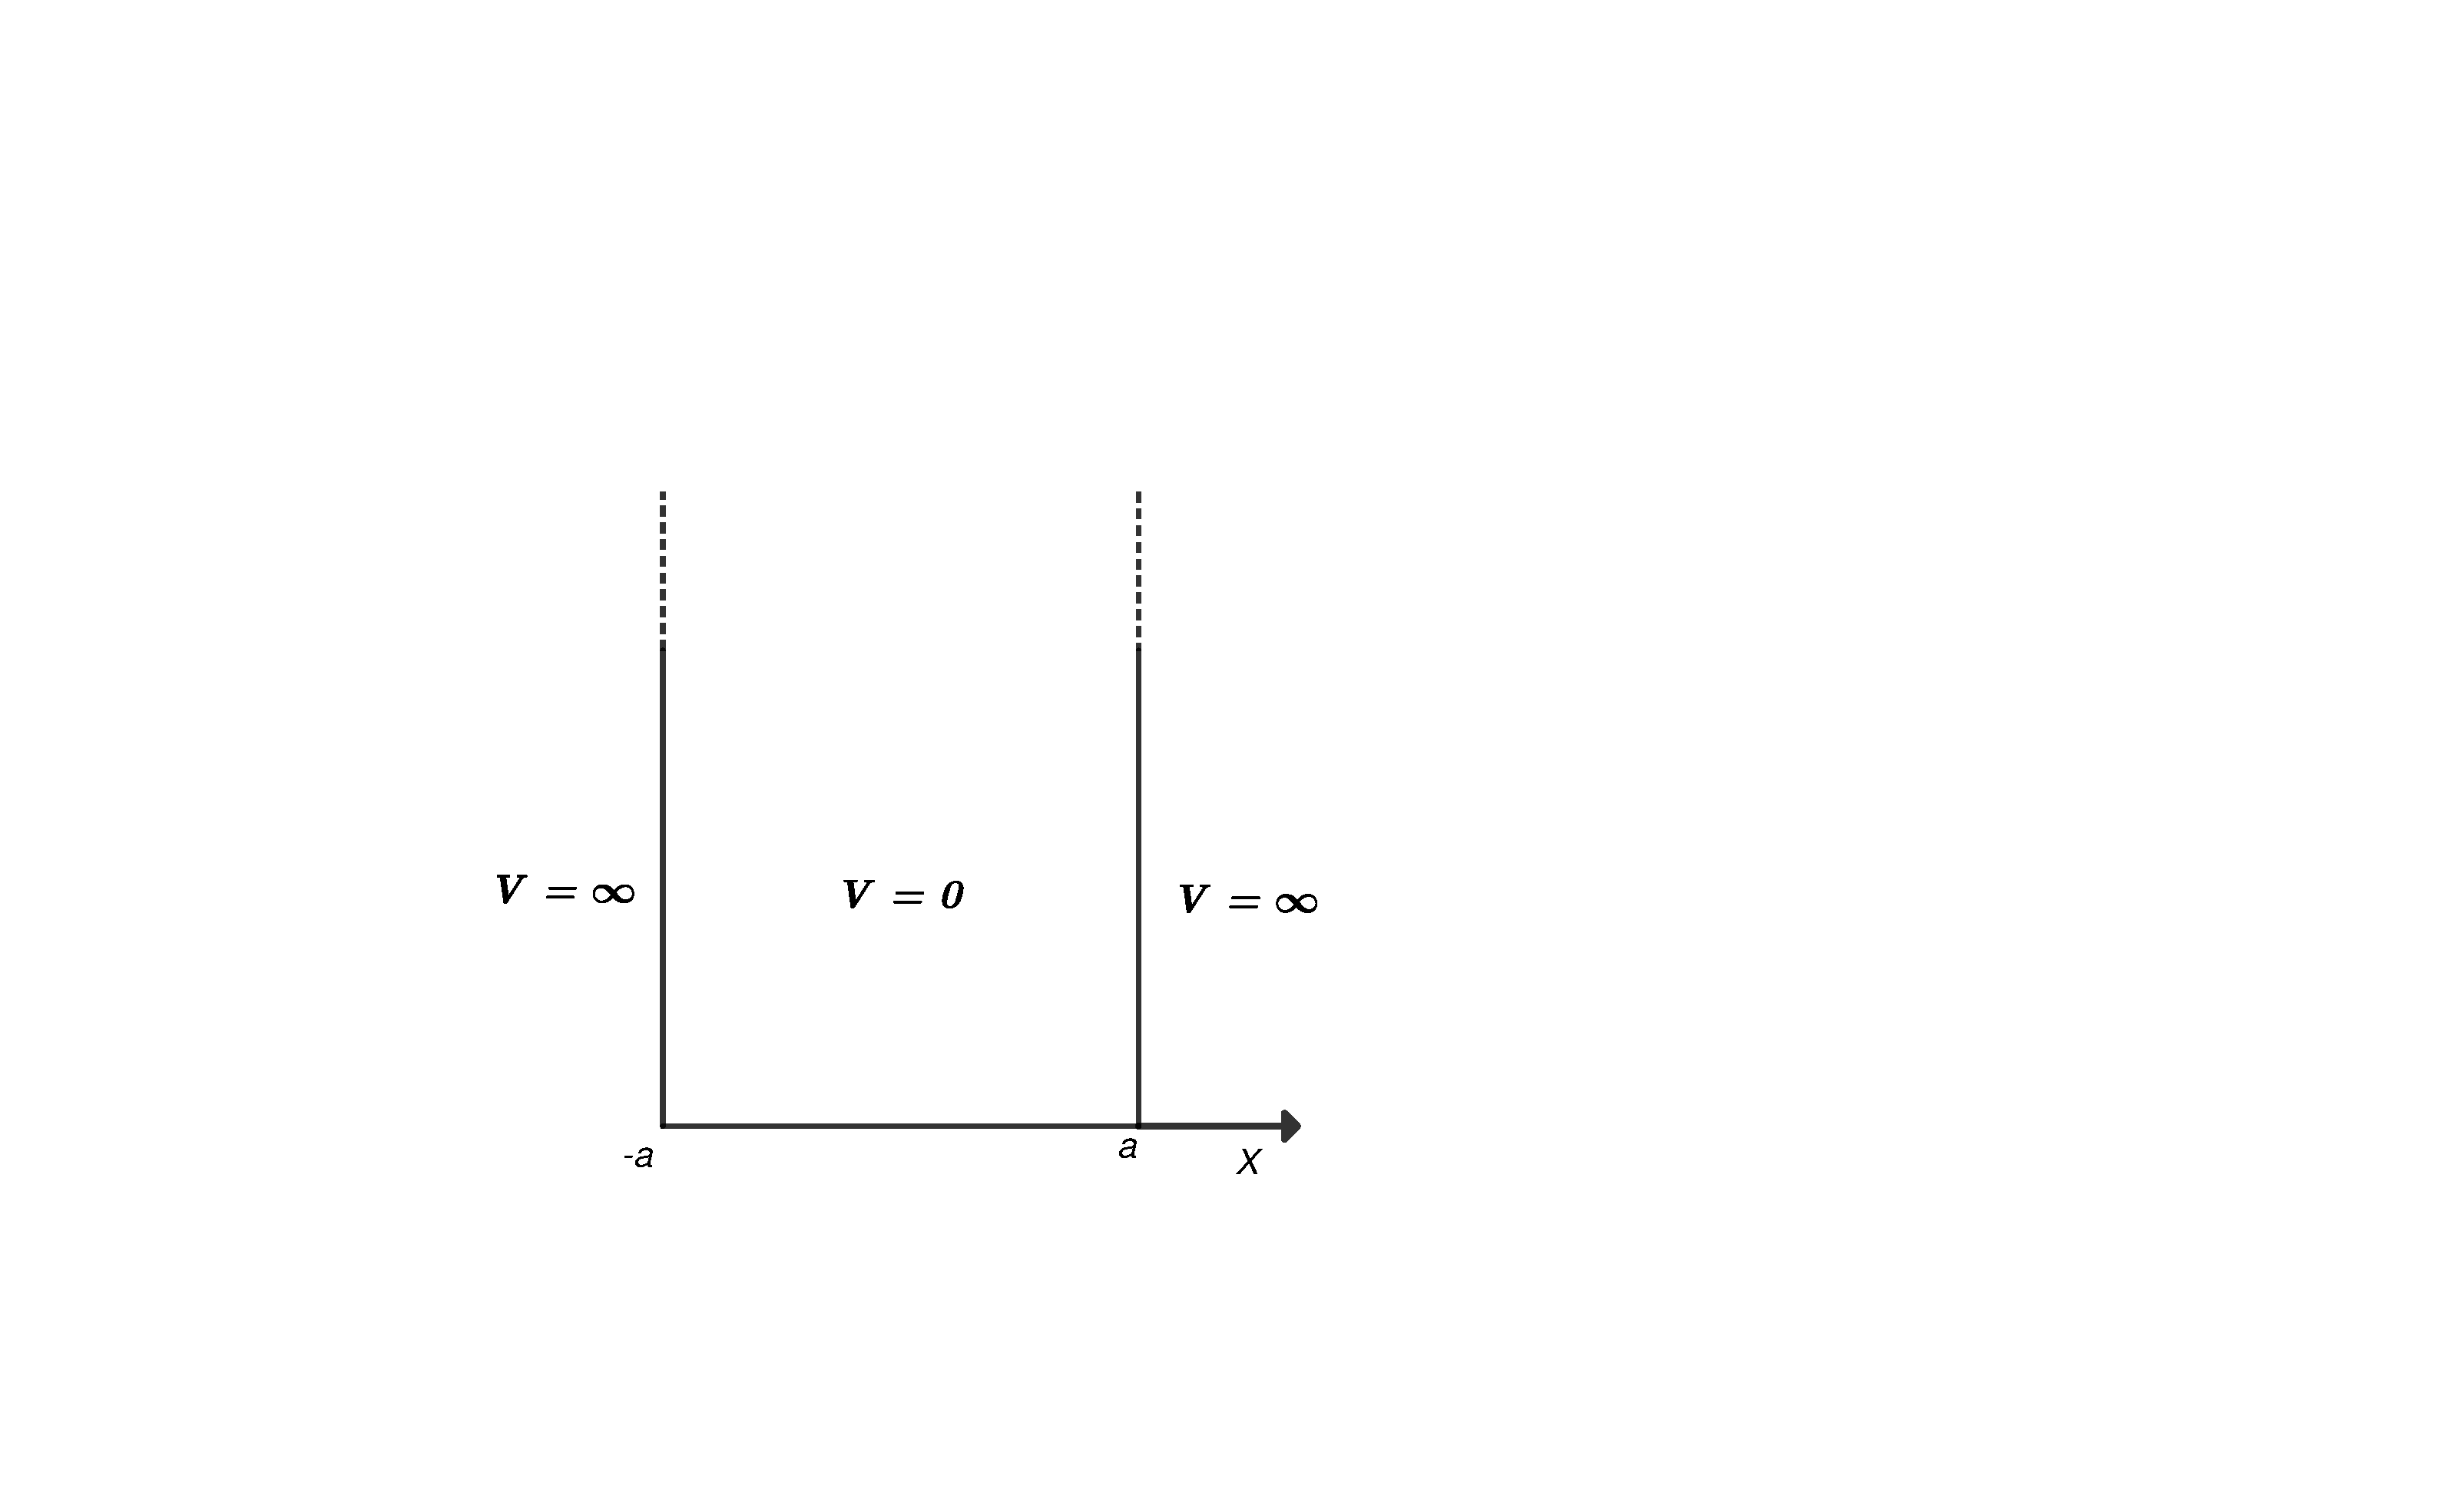
\includegraphics[width=9em]{QM file/figure/2-2}
	\caption{}\label{fig.2-2}
\end{wrapfigure}
如图\ref{fig.2-2}所示.按照$x-V$的图形,这个势场也称为无限深方势阱.粒子在这种势阱中运动时,定态波函数为
\eqlong
\begin{equation}\label{eq24.2}
	\varPsi_{E}(x,t)=\varPsi_{E}(x)e^{-iEt/h}
\end{equation}
$\varPsi_{E}(x)$为空间波函数.由于阱外区域($|x|\geqslant a$)$V=\infty$,$\varPsi$必须等于0,所以可以直接判定
\begin{equation}\label{eq24.3}
	\varPsi_{E}(x)=0,\quad |X|\geqslant a
\end{equation}\eqnormal
阱内$(|x|<a)V=0$,定态薛定谔方程和自由粒子的方程类似,为
\begin{equation}\label{eq24.4}
	\varPsi^{\prime\prime}+k^{2}\varPsi=0,\quad -a<x<a
\end{equation}
其中
\begin{equation}\label{eq24.5}
	k=\frac{\sqrt{2mE}}{\hbar}
\end{equation}
阱内波函数除了满足方程\eqref{eq24.4}外,还要满足边界条件
\begin{equation}\label{eq24.6}
	\varPsi(-a)\approx\varPsi(a)\approx 0
\end{equation}
亦即满足\eqref{eq24.3}式.由于$V(x)$是偶宇称,按照$\S$\ref{sec:02.03}叙述的定理,能量本征态必定有明确的宇称. \eqref{eq24.4}式的特解可以取为$e^{\pm ikx}$或$\cos kx,\sin kx$,前者既不满足边条
件\eqref{eq24.6},也没有宇称性,后二者既有宇称性,也能满足边条件\eqref{eq24.6}.

{\heiti 偶宇称态}

取\eqref{eq24.4}的偶宇称解
\begin{equation*}
	\varPsi(x)=A\cos kx,\quad -a<x<a
\end{equation*}
$A$为归一化系数,边条件\eqref{eq24.6}要求
\begin{equation}\label{eq24.7}
	\cos ka=0,\quad k=\frac{n\pi}{2a},\quad n=1,3,5,\cdots
\end{equation}
因此, 能级为
\begin{equation}\label{eq24.8}
	E_{n}=\frac{\hbar^{2}k^{2}}{2m}=\frac{1}{2m}\bigg(\frac{n\pi\hbar}{2a}\bigg)^{2},\quad
	n=1,3,5,\cdots
\end{equation}
波函数的归一化条件为
\begin{equation}\label{eq24.9}
	\int_{-\infty}^{\infty} |\varPsi|^{2}dx=\int_{-a}^{a} \varPsi^{2}dx=1
\end{equation}
由此定出$A=\frac{1}{\sqrt{a}}$,所以归一化的能量本征函数为
\begin{equation}\label{eq24.10}
	\varPsi_{n}(x)\approx \frac{1}{\sqrt{a}}\cos\frac{n\pi x}{2a},\quad n=1,3,5,\cdots
\end{equation}

{\heiti 奇宇称态}

取\eqref{eq24.4}式的奇宇称解
\begin{equation*}
	\varPsi(x)=A\sin kx,\quad -a<x<a
\end{equation*}
由边条件\eqref{eq24.6}得出
\begin{equation}\label{eq24.11}
	\sin ka=0,\quad k=\frac{n\pi}{2a},\quad n=2,4,6,\cdots
\end{equation}
因此能级为
\begin{equation}\label{eq24.12}
	E_{n}=\frac{1}{2m}\bigg(\frac{n\pi\hbar}{2a} \bigg)^{2},\quad n=2,4,6,\cdots
\end{equation}
归一化的本征函数为
\begin{equation}\label{eq24.13}
	\varPsi_{n}(x)=\frac{1}{\sqrt{a}}\sin\frac{n\pi x}{2a},\quad n=2,4,6,\cdots
\end{equation}
由于粒子被限制在$-a<x<a$范围内运动,只有束缚态,没有游离态,所以全部能级都是量子化的,能级公式为\eqref{eq24.8}、\eqref{eq24.12}式.

$\varPsi_{n}(x)$的图形如图\ref{fig.2-3}所示.在$(-a,a)$间形成驻波,波长为
\begin{equation}\label{eq24.14}
	\lambda=\frac{2\pi}{k}=\frac{4a}{n},\quad n=1,2,3\cdots
\end{equation}
注意$\varPsi_{n}(x)$有$(n + 1)$个波节($\varPsi$的零点).

{\heiti 2.有限深平底势阱}

也称有限深方势阱,势能为
\begin{equation}\label{eq24.14'}
	V(x)=
	\begin{cases} \notag
		-V_{0}, &|X|<a \\
		0,	 &|X|\geqslant a
	\end{cases} \tag{$2.4.14^{\prime}$}
\end{equation}
如图\ref{fig.2-4}所示这种势场可以作为许多实际问题中势场的简单模型,金属中的“自由电子”,原子核中的核子,它们所处的等效势场都可用\eqref{eq24.14}式近似表示,$V_{0}$称为势阱的深度,$2a$是阱的宽度.势能的最小值就是阱内势能$-V_{0}$,由于粒子的定态能量必须大于$V(x)$的平均值,所以$E>-V_{0}$.定态波函数仍可表示成
\begin{equation*}
	\varPsi_{E}(x,t)=\varPsi_{E}(x)e^{-iEt/h}
\end{equation*}
在阱内和阱外,定态薛定谔方程具有不同的构造.
\begin{figure}
	\centering
	\begin{minipage}[h!]{12em}
		\centering
		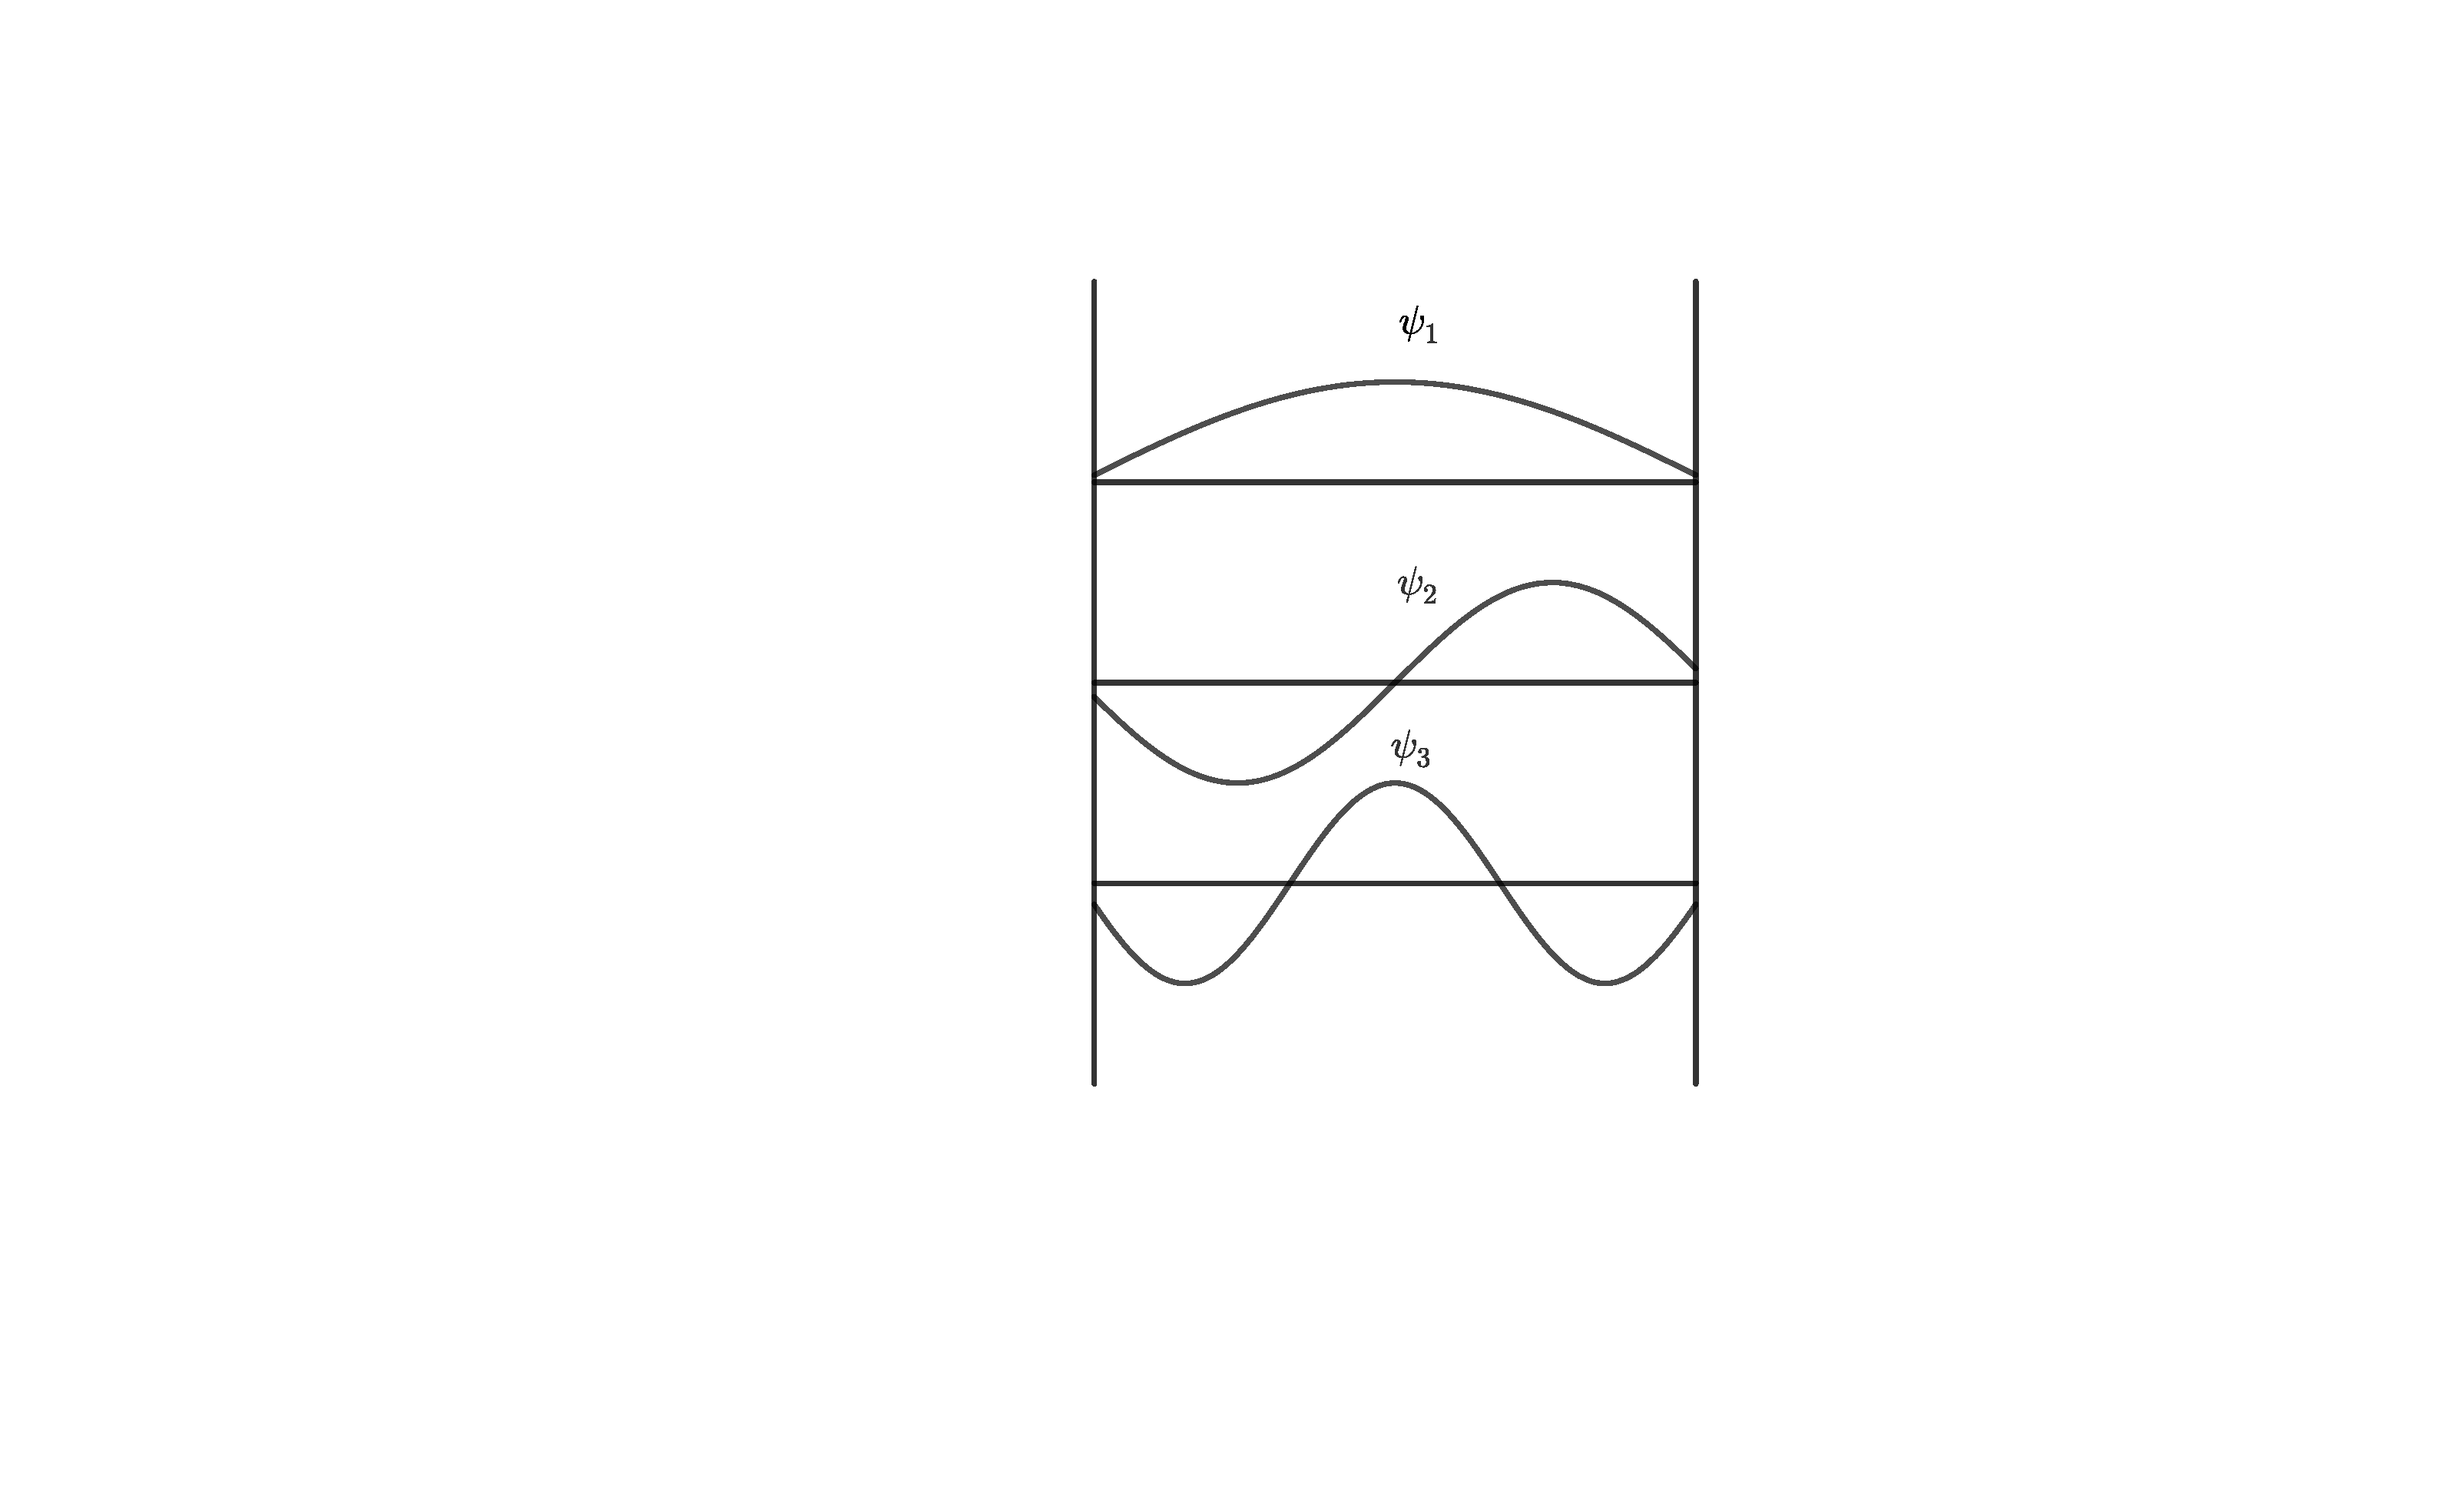
\includegraphics[width=9em]{QM file/figure/2-3}
		\caption{}\label{fig.2-3}
	\end{minipage}
	\begin{minipage}[h!]{12em}
		\centering
		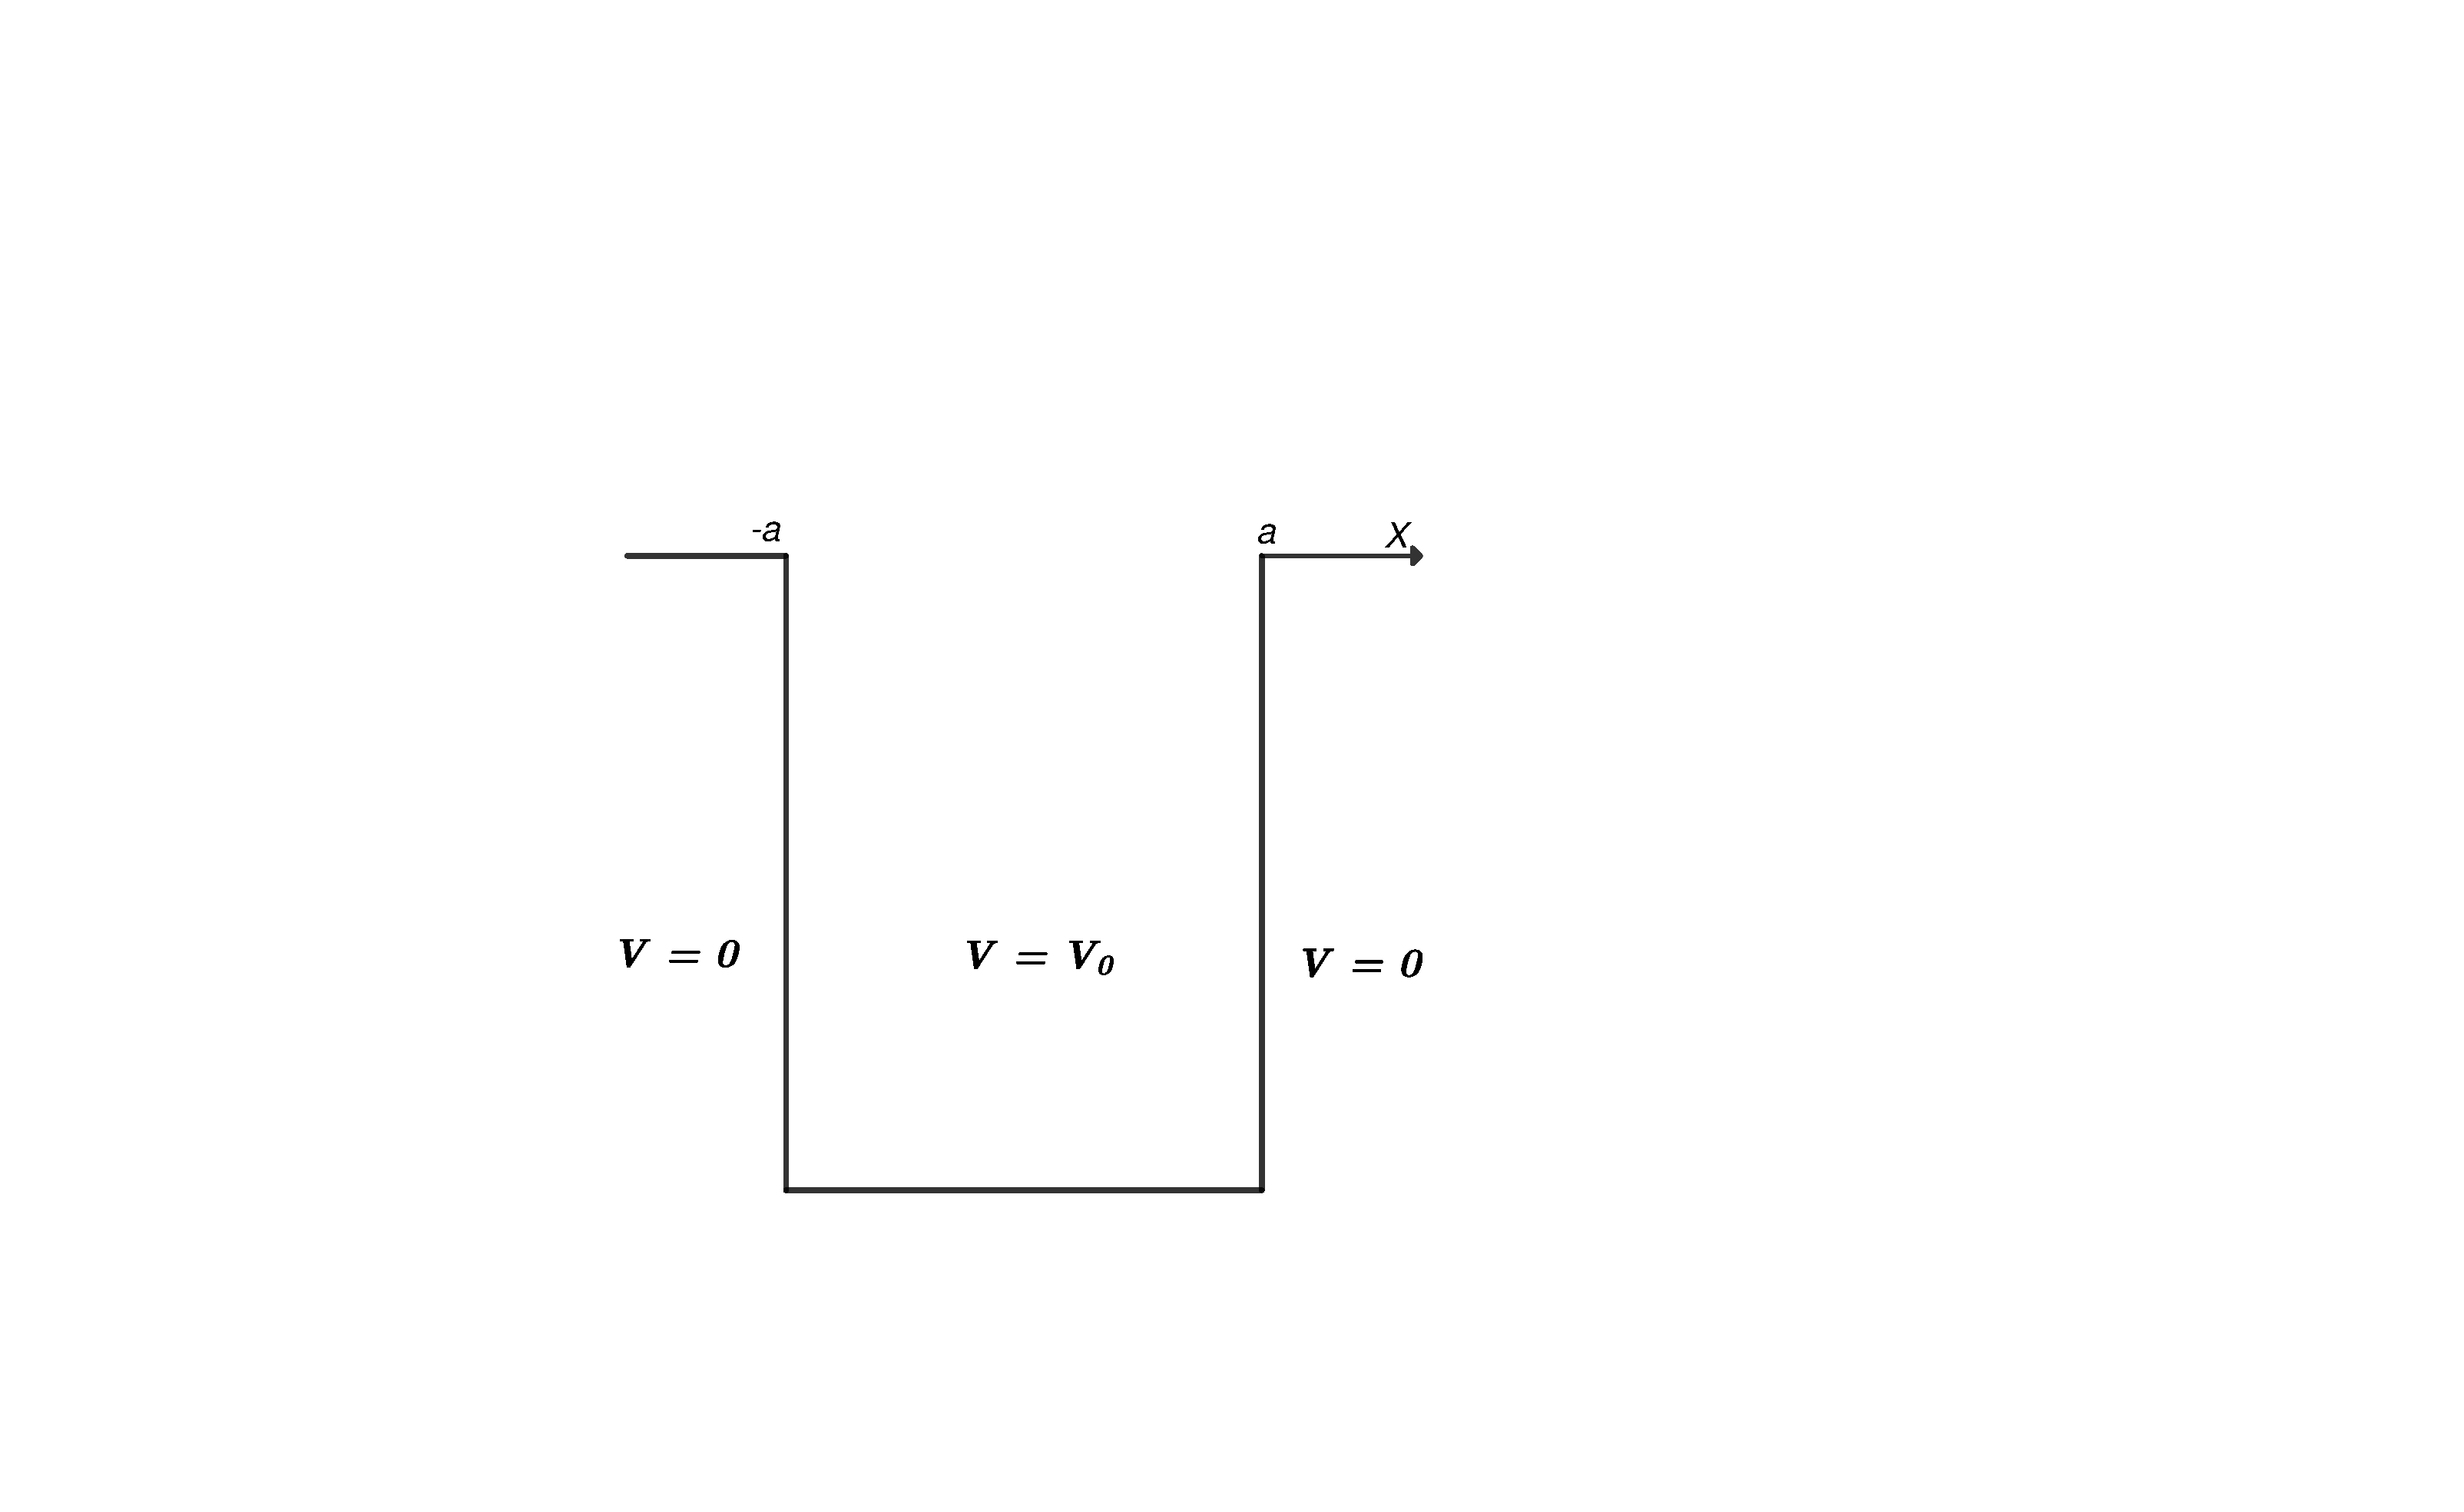
\includegraphics[width=9em]{QM file/figure/2-4}
		\caption{}\label{fig.2-4}
	\end{minipage}
\end{figure}

阱外$(|x|\geqslant a)$.$V(x)=0$ ,定态薛定谔方程为
\begin{equation}\label{eq24.15}
	\varPsi^{\prime\prime}+\frac{2mE}{\hbar^{2}}\varPsi=0,\quad |x|\geqslant a
\end{equation}

阱内$|x|<a$.$V(x)=-V_{0}$,定态薛定谔方程为
\begin{equation}\label{eq24.16}
	\varPsi^{\prime\prime}+\frac{2mE}{\hbar^{2}}(E+V_{0})=0,\quad |x|\geqslant a
\end{equation}
由于$E>-V_{0},E+V_{0}>0$,令
\begin{equation}\label{eq24.17}
	k=\frac{\sqrt{2}m(E+V_{0})}{\hbar}
\end{equation}
则\eqref{eq24.16}式可以写成
\begin{equation*}\label{eq24.16'}
	\varPsi^{\prime\prime}+k^{2}\varPsi=0	\tag{$2.4.16^{\prime}$}
\end{equation*}
和无限深势阱的\eqref{eq24.4}式相似($k$的定义不同).\eqref{eq24.16'}式的两个基本解可以取为$\cos kx$和$\sin kx$元,前者为偶宇称,后者为奇宇称.

对于\eqref{eq24.15}式,$E>0$和$-V_{0}<E<0$有本质区别,前者为游离态,后者为束缚态.我们将着重讨论束缚态.

由于$V(x)$取有限值,$\varPsi(x)$及$\varPsi^{\prime}(x)$是全空间的连续函数,因此由\eqref{eq24.15}式及\eqref{eq24.16'}式分别求出的$\varPsi(x)$及其微商$\varPsi^{\prime}(x)$在$x=\pm a$处应该满足连续条件,以$x=a$处为例, 连续条件为
\setlength{\mathindent}{5em}
\begin{equation*}\label{eq24.17'}
	\varPsi(a-0)=\varPsi(a+0),\quad \varPsi^{\prime}(a-0)=\varPsi^{\prime}(a+0)
	\tag{$2.4.17^{\prime}$}
\end{equation*}\eqnormal
$\varPsi(a\pm 0)$表示,$\varPsi(a\pm\varepsilon),\varepsilon\rightarrow 0$.

{\heiti 束缚态$(-V_{0}<E<0)$}

令
\begin{equation}\label{eq24.18}
	\beta=\frac{\sqrt{-2mE}}{\hbar}>0
\end{equation}
\eqref{eq24.15}式简化成
\begin{equation*}\label{eq24.15'}
	\varPsi^{\prime\prime}\-\beta^{2}\varPsi=0,\quad |x|\geqslant a	\tag{$2.4.15^{\prime}$}
\end{equation*}
两个特解为$e^{\beta x},e^{-\beta x}$.为了保证$\varPsi(x)$有限,必须取
\begin{equation}\label{eq24.19}
	\varPsi(x)=
	\begin{cases}
		Ce^{-\beta x},  & x\geqslant a 		\\
		C^{\prime}e^{\beta x},	& x\leqslant -a
	\end{cases}
\end{equation}
即阱外波函数为指数衰减型这样,当$x\rightarrow\pm\infty$,$\varPsi(x)$迅速趋于0,$ \varPsi(x) $可以满足归一化条件,所以是束缚态.

{\heiti 偶宇称态}$\varPsi(x)\approx\varPsi(-x)$

波函数(不管归一化条件)为
\begin{equation}\label{eq24.20}
	\varPsi(x)=
	\begin{cases}
		Ce^{-\beta x},  & x\geqslant a 		\\
		\cos kx,		& -a<x<a		\\
		Ce^{\beta x},	& x\leqslant -a
	\end{cases}
\end{equation}
利用$ x=a $处$ \varPsi $及$ \varPsi^{\prime} $的连续条件\eqref{eq24.17'},得到
\begin{align}
	C^{-\beta a} &=\cos ka \label{eq24.21} \\
	-\beta Ce^{-\beta a} &=-k\sin ka \label{eq24.22}
	\intertext{二式相除,得到}
	k\tan ka &=\beta	\label{eq24.23}
\end{align}
由于$ K $及$ \beta $均为$ E $的函数,所以\eqref{eq24.23}是$E$所满足的一个超越方程.另外,从$k$和$\beta$的定义式\eqref{eq24.17}、\eqref{eq24.18}还可看出,$k$和$\beta$满足关系
\begin{equation}\label{eq24.24}
	k^{2}+\beta^{2}=\frac{2mV_{0}}{\hbar^{2}}
\end{equation}
\eqref{eq24.23}和\eqref{eq24.24}式就是决定$k$和$\beta$的方程,亦即能级方程,如令
\begin{equation}\label{eq24.25}
	{}
	\begin{cases}
		\xi=ka=\frac{a}{\hbar}\sqrt{2}m(E+V_{0})>0 \\
		\eta=\beta a=\frac{a}{\hbar}\sqrt{-2mE}>0
	\end{cases}
\end{equation}
则能级方程可以写成
\begin{empheq}[left=\empheqlbrace]{align*}
	&\xi\tan\xi=\eta	\tag{$2.4.23^{\prime}$}	\label{eq24.23'}	\\
	&\xi^{2}+\eta^{2}=\frac{2mV_{0}a^{2}}{\hbar^{2}}	\tag{$2.4.24^{\prime}$} \label{eq24.24'}
\end{empheq}
\eqref{eq24.20}式中系数$C$可以由\eqref{eq24.21}式定出,
\begin{equation*}
	C=\cos kae^{\beta_{0}}=\cos\xi\cdot e^{\eta} \tag{$2.4.21^{\prime}$}
\end{equation*}

{\heiti 奇宇称态}$\varPsi(-x)\approx-\varPsi(x)$

波函数为
\begin{equation}\label{eq24.26}
	\varPsi(x)=
	\begin{dcases}
		C^{\prime}e^{-\beta x},  & x\geqslant a 		\\
		\sin kx,		& -a<x<a		\\
		-C^{\prime}e^{\beta x},	& x\leqslant -a
	\end{dcases}
\end{equation}
类似的步骤求得
\setlength{\mathindent}{12em}
\begin{align}
	& \xi\cos\xi=-\eta \label{eq24.27}	\\
	& C^{\prime}=\sin\xi\cdot e^{\eta}	\label{eq24.28}
\end{align}
\eqnormal
\eqref{eq24.27}式和\eqref{eq24.24'}式一起构成能级方程.

{\heiti 能谱}

能级方程\eqref{eq24.23'},\eqref{eq24.24'}.\eqref{eq24.27}可以用数值解法或图解法处理.下面介绍图解法.在$\xi-\eta$图上将\eqref{eq24.23'}、\eqref{eq24.27}式和\eqref{eq24.24'}式分别画成曲线,它们的交点所对应的$\eta$值就代表[通过\eqref{eq24.25}式]能量特征值.
\begin{figure}[!h]
	\centering
	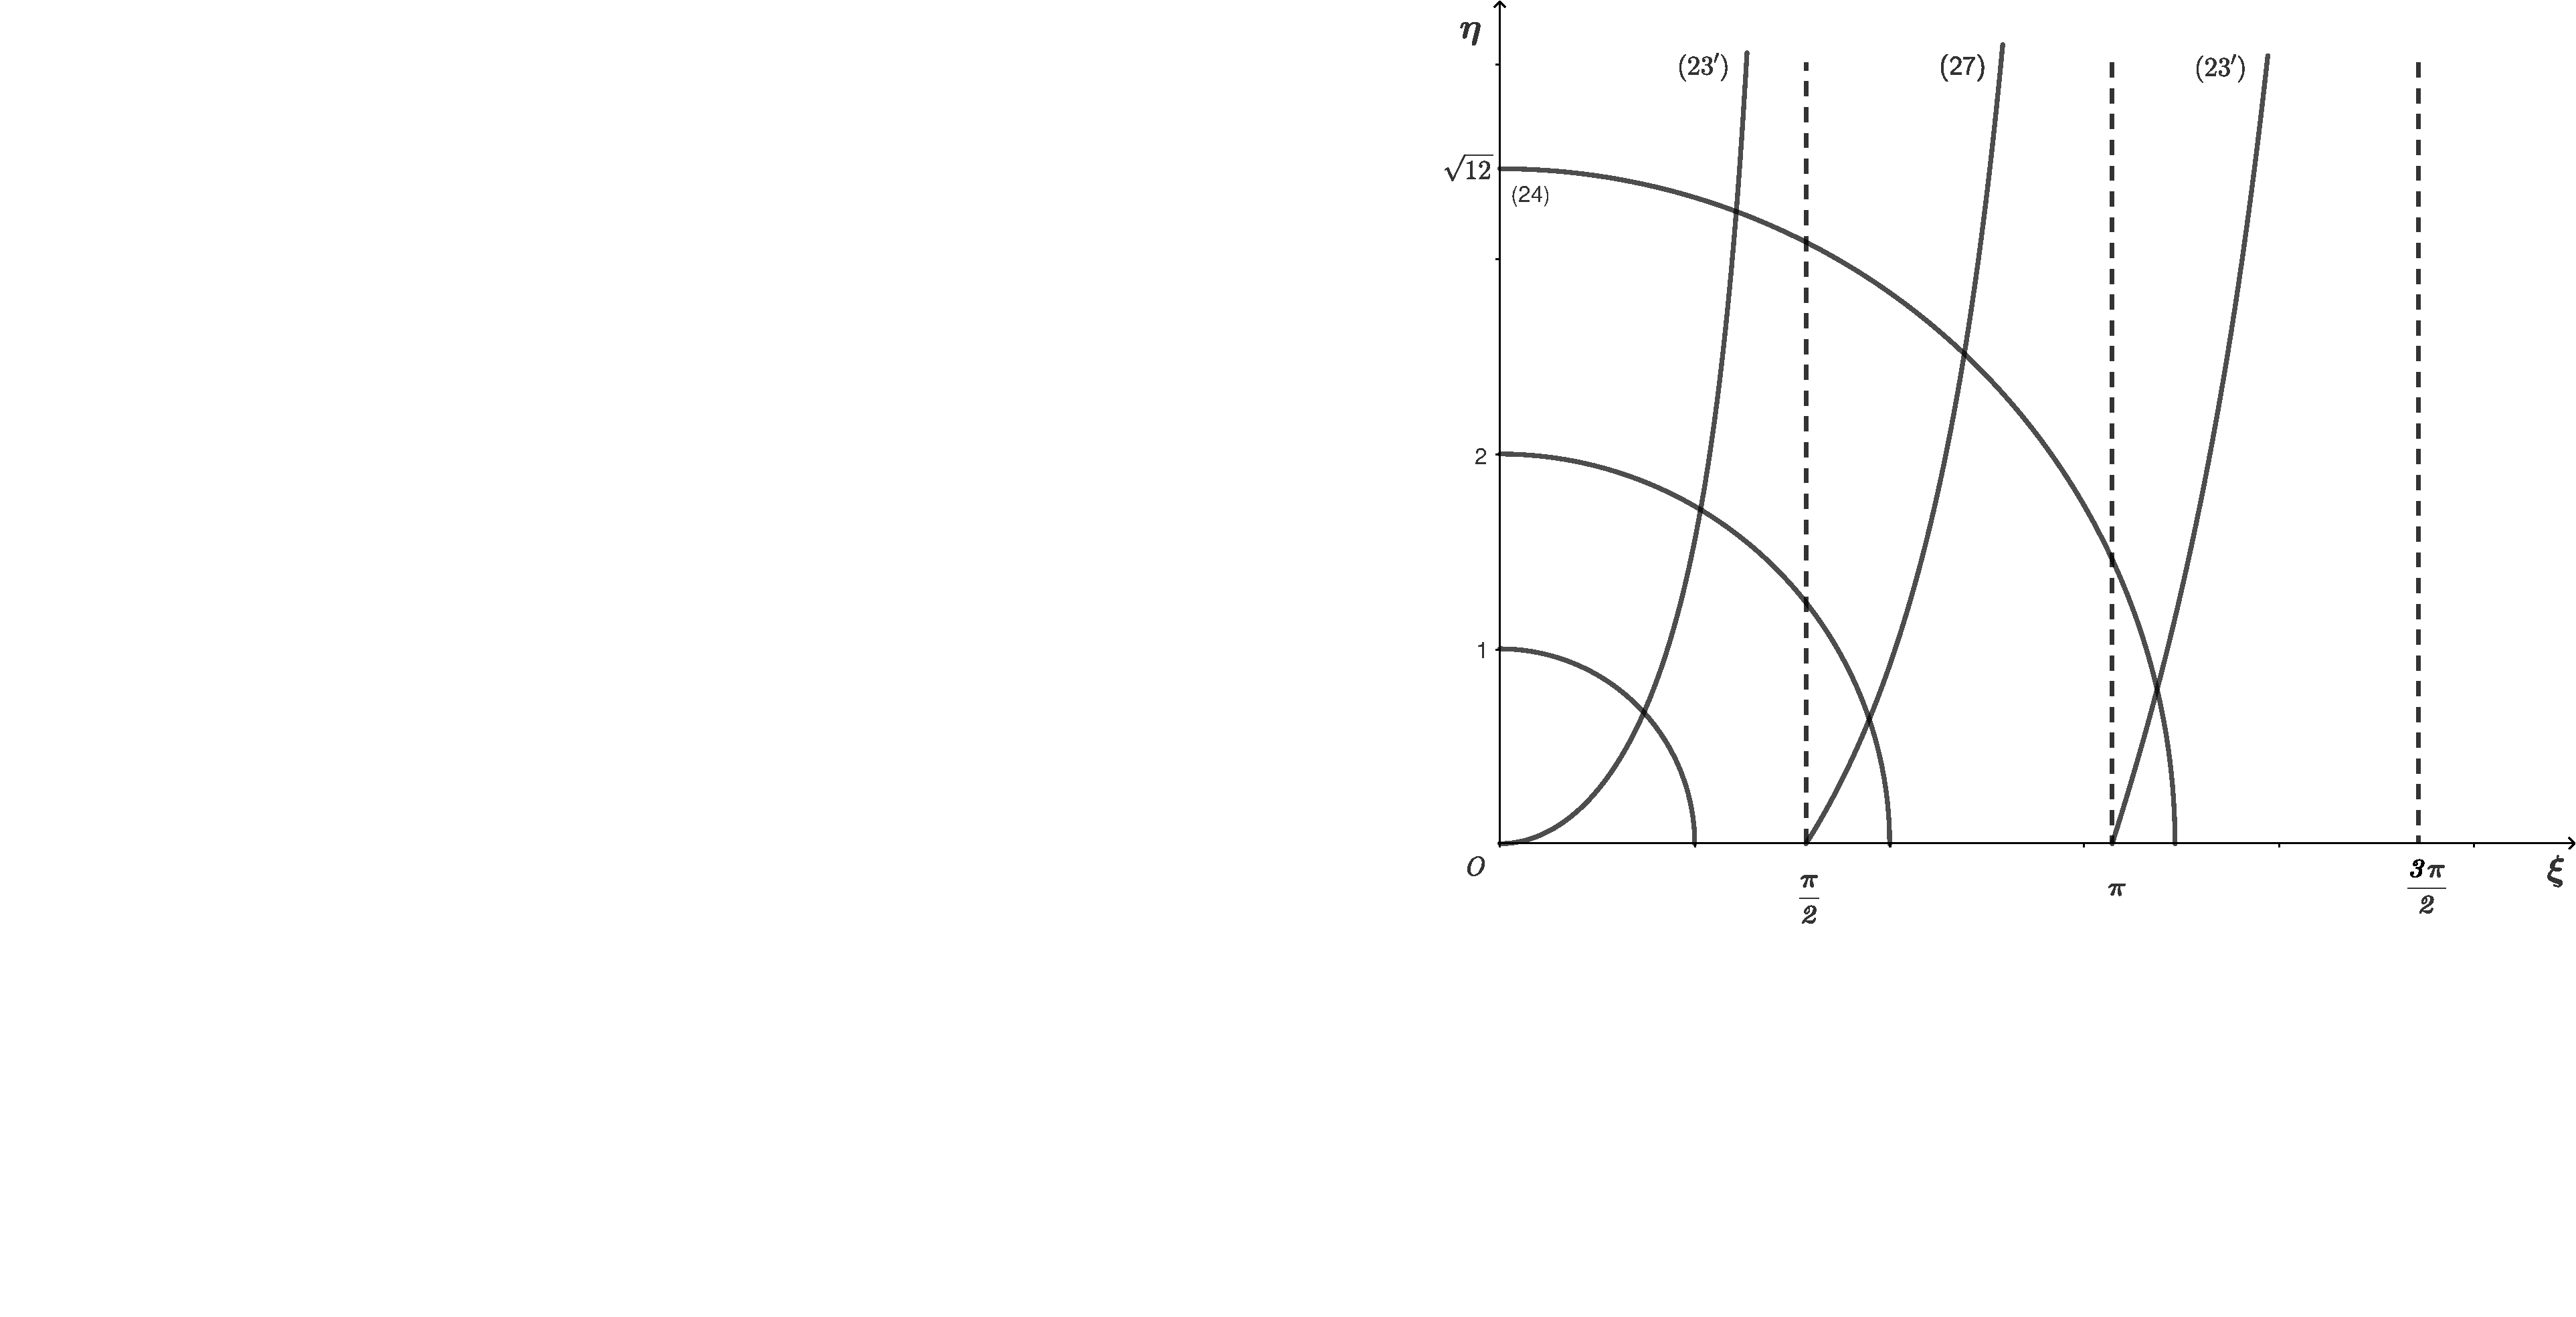
\includegraphics[width=4cm,clip]{QM file/figure/2-5}
	\caption{}\label{fig.2-5}
\end{figure}
束缚态能谱完全取决于$\dfrac{2mV_{0}a}{\hbar}$的数值.图\ref{fig.2-5}就$\dfrac{2mV_{0}a}{\hbar}$的三种特殊值给出了$(\xi,\eta)$值的图解.精确的数值可由数值解法求出,如表\ref{lab.2-1}所示.
\begin{table}[!h]
	\begin{center}
		\caption{}\label{lab.2-1}
		\begin{tabular}{c|c|c|c|c|c}
			\hline 
			\multirow{2}{*}{$\dfrac{2mV_{0}a}{\hbar}$} & \multirow{2}{*}{$\xi$} & \multirow{2}{*}{$\eta$} & \multirow{2}{*}{宇称} & \multirow{2}{*}{$E_{n}$(能级编号)} & \multirow{2}{*}{$\dfrac{4\xi^{2}}{n^{2}\pi^{2}}$} \\ 
			&  &  &  &  &  \\ \hline
			1 & 0.7391 & 0.6736 & 偶 & $E_{1}$ & 0.2214 \\ \hline
			\multirow{2}{*}{4} & 1.0299 & 1.7145 & 偶 & $E_{1}$ & 0.4299 \\ \cline{2-6}
			& 1.895 & 0.6380 & 奇 & $E_{2}$ & 0.3640 \\ \hline
			\multirow{3}{*}{12} & 1.2130 & 3.2448 & 偶 & $E_{1}$ & 0.5964 \\ \cline{2-6}
			& 2.3830 & 2.5142 & 奇 & $E_{2}$ & 0.5754 \\ \cline{2-6}
			& 3.3723 & 0.7922 & 偶 & $E_{3}$ & 0.5121 \\ \hline
			\multirow{2}{*}{$\bigg(\dfrac{10\pi}{2}\bigg)^{2}$} & 1.4767 & 15.6384 & 偶 & $E_{1}$ & 0.8837 \\ \cline{2-6}
			& 2.9525 & 15.4280 & 奇 & $E_{2}$ & 0.8832 \\ \hline
		\end{tabular}
	\end{center}
\end{table}

由能级方程、图\ref{fig.2-5}和表\ref{lab.2-1}可以看出,有限深平底势阱的能级构造有以下规律:

(1) 偶宇称态至少有一个能级.$\dfrac{2mV_{0}a^{2}}{\hbar^{2}}$,能级总数越多. 相邻的能级,宇称相反. 基态能级为偶宇称.

(2) 从阱底算起的能级高度$(V_{0}+E\propto\xi^{2})$低于无限深势阱的相应能级高度.\ref{lab.2-1}最后一列是两种势阱能级高度的比值.当$\dfrac{2mV_{0}a^{2}}{\hbar^{2}}$逐渐增大时,能级总数越来越多,最低的那些能级$\bigg(n\leqslant\dfrac{2a\sqrt{2mV_{0}}}{\pi\hbar}\bigg)$高度逐渐接近无限深势阱的能级高度.

(3) 从阱口算起的能级深度$(-E\propto\eta^{2})$随$\dfrac{2mV_{0}a^{2}}{\hbar^{2}}$增加而增加.每当$\dfrac{2mV_{0}a^{2}}{\hbar^{2}}$超过$\bigg(\dfrac{n\pi}{2}\bigg)^{2}$,阱口即出现一个新能级$(E_{n+1}\sim 0^{-})$能级总数等于
\begin{empheq}{equation}\label{eq24.29}
	n_{max}=1+\big[\frac{2a\sqrt{2mV_{0}}}{\pi\hbar}\big]
\end{empheq}
$[x]$表示不大于$x$的最大整数.

{\heiti 3. $\delta$势阱}

对于有限深方势阱\eqref{eq24.14}式,显然
\begin{empheq}{equation}\label{eq24.30}
	\int_{-\infty}^{\infty}V(x)dx=-2V_{0}a \overset{\text{定义}}{=} -\gamma
\end{empheq}
如果$V_{0}\rightarrow\infty,a\rightarrow 0$,同时保持$\gamma=2V_{0}$.$a$为有限值,就得到一个无限深而又无限窄并满足\eqref{eq24.30}式的势阱,称为$\delta$势阱,其$V(x)$可以写成
\begin{empheq}{equation}\label{eq24.31}
	V(x)=-\gamma\delta(x),\quad\gamma>0
\end{empheq}
由于仅当$ x=0 $,$\delta(x)$才不为0,而且
\begin{empheq}{equation}\label{eq24.32}
	\int_{-\infty}^{\infty}\delta(x)dx=1
\end{empheq}
所以由\eqref{eq24.31}式定义的$ V(x) $显然满足\eqref{eq24.30}式.

在$\delta$势阱中运动的粒子,参量$\frac{2mV_{0}a^{2}}{\hbar^{2}}\rightarrow 0$,所以只有一个束缚态$(E<0)$,波函数为偶宇称,满足定态薛定谔方程
\begin{empheq}{equation}\label{eq24.33}
	\varPsi^{\prime\prime}+\frac{2m\gamma}{\hbar^{2}}\delta(x)\varPsi+\frac{2mE}{\hbar^{2}}\varPsi=0
\end{empheq}
对上式积分,$\int_{-\varepsilon}^{\varepsilon}\cdots dx$,并令$\varepsilon\rightarrow 0$,得到
\setlength{\mathindent}{4em}
\begin{empheq}{equation}\label{eq24.34}
	\varPsi^{\prime}(0^{+})-\varPsi(0^{-})=-\frac{2m\gamma}{\hbar^{2}}\int_{-\varepsilon}^{\varepsilon}\delta(x)\varPsi(x)dx=-\frac{2m\gamma}{\hbar^{2}}\varPsi(0)
\end{empheq}
\eqnormal
$\varPsi^{\prime}$即$\varPsi^{\prime}(\pm\varepsilon)$,$\varepsilon\rightarrow 0$.由上式可见,如$\varPsi\neq 0$,则在$x=0$处$\varPsi$的左微商和右微商不相等,亦即$x=0$处$\varPsi^{\prime}$产生跃变.在$x\neq 0$处,$\delta(x)=0$,\eqref{eq24.33}式成为
\begin{empheq}{equation}\label{eq24.35}
	\varPsi^{\prime\prime}-\beta^{2}\varPsi=0,\quad \beta=\frac{\sqrt{-2mE}}{\hbar}>0
\end{empheq}
其特解为$e^{\pm\beta x}$,考虑到$x\rightarrow\pm\infty$处,$\varPsi$必须有限,所以
\begin{empheq}{equation*}
	x>0,\varPsi\sim e^{-\beta x};\quad x<0,\varPsi\sim e^{\beta x}
\end{empheq}

{\heiti 偶宇称态}

取\eqref{eq24.35}式的偶宇称解
\begin{align}\label{eq24.36}
	\varPsi(x)=
	\begin{dcases}
		Ae^{-\beta x},	&x>0	\\
		Ae^{-\beta x},	&x<0
	\end{dcases}
\end{align}
其微商为
	\begin{numcases}
		{\varPsi^{\prime}(x)=}
		-A\beta e^{-\beta x},	&\text{$x>0$}	\notag	\\
		A\beta e^{-\beta x},	&\text{$x<0$} \notag
	\end{numcases}
令$x\rightarrow 0$.利用$\varPsi^{\prime}$跃变条件\eqref{eq24.34},容易求出
\begin{equation} \label{eq24.37}
	\beta=\frac{\sqrt{-2mE}}{\hbar}=\frac{m\gamma^{2}}{\hbar^{2}}	
\end{equation}
因此能级为
\begin{equation} \label{eq24.38}
	E=-\frac{\hbar^{2}\beta^{2}}{2m}=-\frac{m\gamma^{2}}{2\hbar}	
\end{equation}
\eqref{eq24.36}式中$A$为归一化常数,利用归一化条件
\begin{empheq}{equation*}
	\int_{-\infty}^{\infty}\varPsi^{2}dx=1
\end{empheq}
容易求出$A=\sqrt{\beta}$,因此归一化的能量本征函数为
\begin{align*}\label{eq24.36'}
	\varPsi(x)=
	\begin{dcases}\notag
		\sqrt{\beta}e^{-\beta x}, &x>0	\\ \tag{$2.4.36^{\prime}$}
		\sqrt{\beta}e^{\beta x}, &x<0
	\end{dcases}
\end{align*}
\begin{wrapfigure}[10]{r}{7em}
	\centering
	\small
	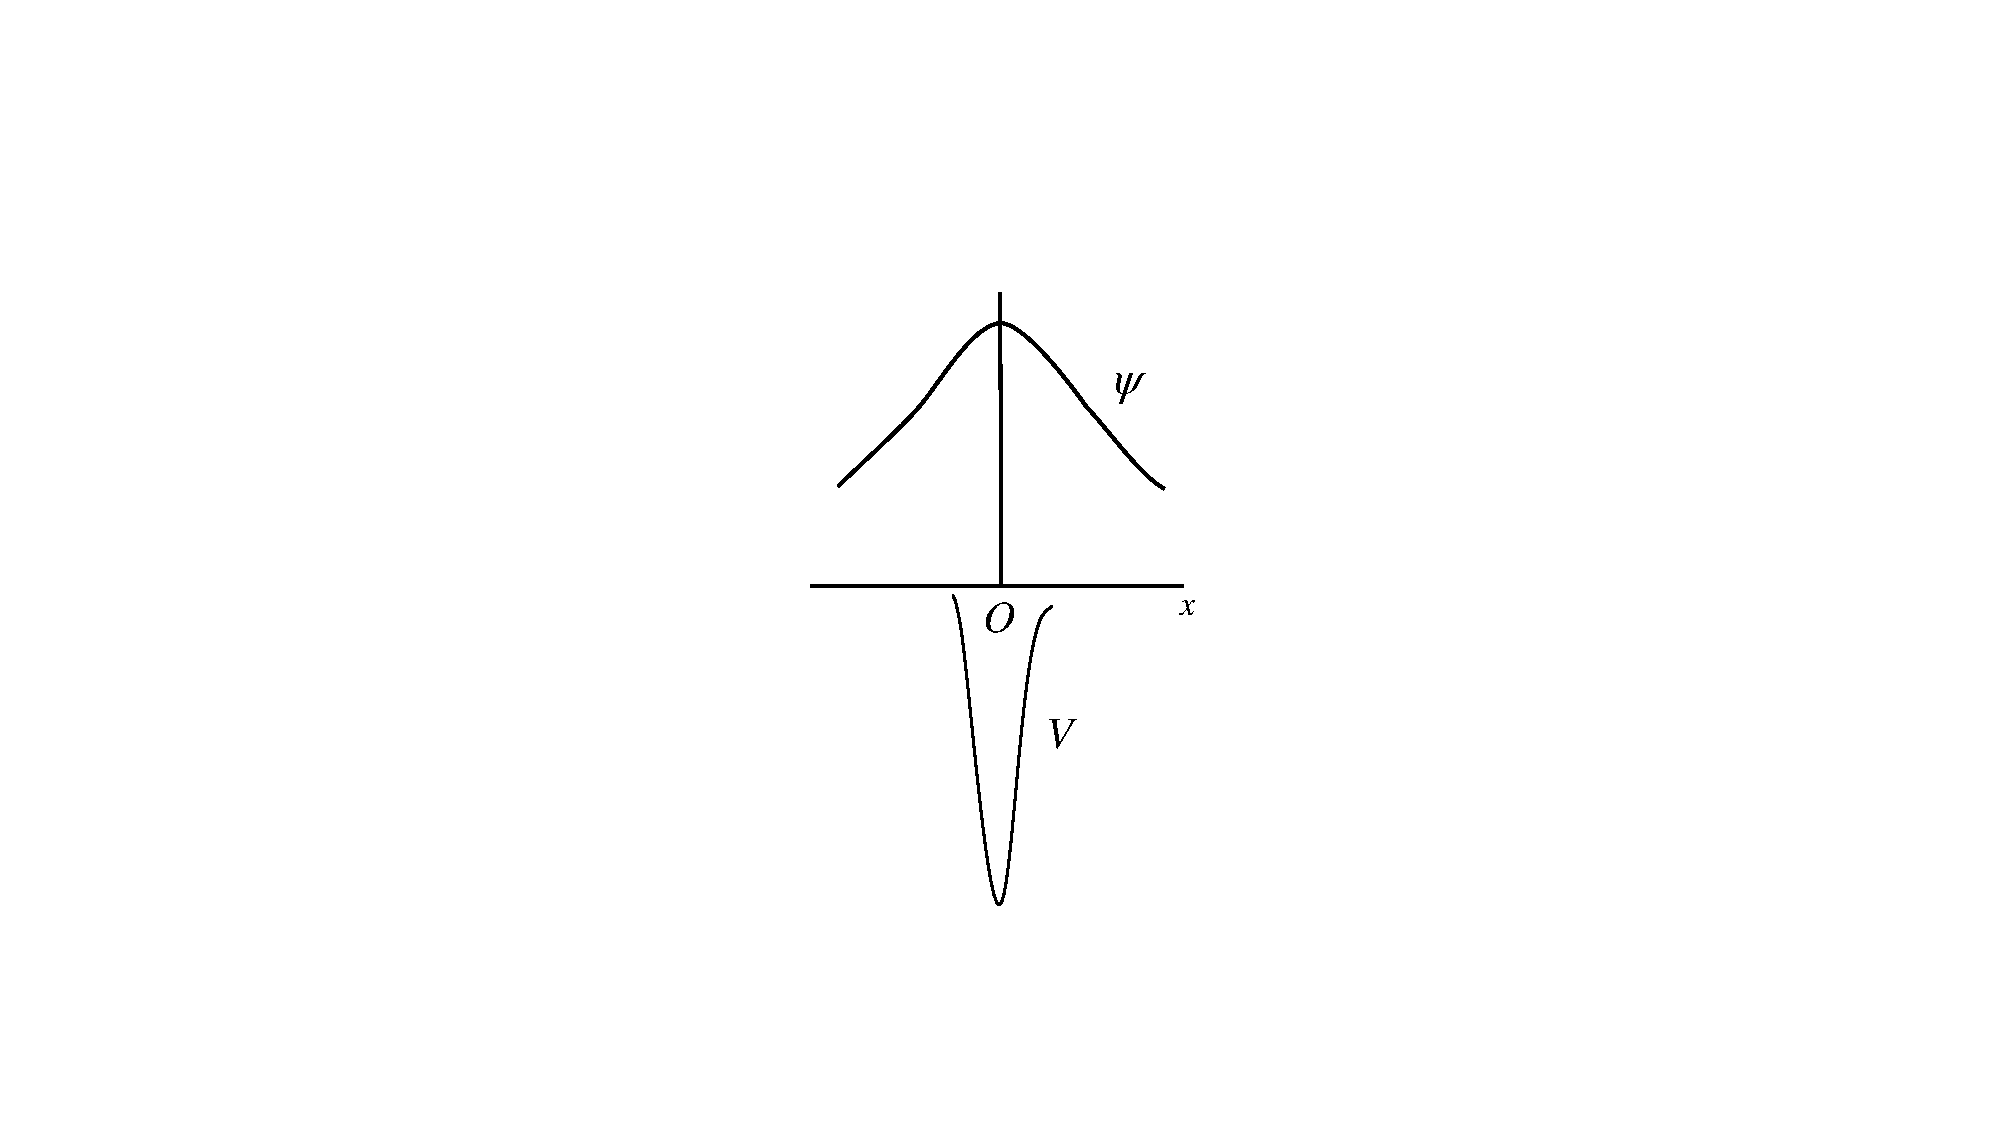
\includegraphics[width=7em,height=9em]{QM file/figure/2-6}
	\caption{}\label{fig.2-6}
\end{wrapfigure}
$\varPsi$的图形如图\ref{fig.2-6}所示,这是$\delta$势阱中的唯一束缚态.

{\heiti 奇宇称态}

\eqref{eq24.35}式的奇宇称解为
\eqlong
\begin{empheq}{equation*}
	{\varPsi(x)=}
	\begin{dcases}
		Be^{-\beta x}	\\
		-Be^{\beta x}
	\end{dcases}
\end{empheq}\eqnormal
满足$\varPsi(-x)=-\varPsi(x)=$.当$x\rightarrow 0,\varPsi(0)=0$,因此$B=0$,即$\varPsi(x)=0$.因此奇宇称束缚态并不存在原因在于:奇宇称态波函数满足$\varPsi(0)=0$,\eqref{eq24.33}式中$\delta(x)$项效果为0,亦即$\delta$势阱对奇宇称态不起作用,粒子运动与自由运动无异,因此$E>0$不存在束缚态.

表征$\delta$势阱性质的特征长度是
\begin{empheq}{equation}\label{eq24.39}
	\frac{1}{\beta}=\frac{\hbar^{2}}{m\gamma}
\end{empheq}
由\eqref{eq24.36'}式容易算出粒子在$|x|<\frac{1}{\beta}$范围内出现概率为
\setlength{\mathindent}{5em}
\begin{empheq}{equation}\label{eq24.40}
	\int_{\frac{1}{\beta}}^{-\frac{1}{\beta}}\varPsi^{2}dx
	=2\beta\int_{0}^{\frac{1}{\beta}}e^{-2\beta x}dx
	=1-e^{-2}=0.8647
\end{empheq}\eqnormal

\example 试利用有限深势阱能级方程导出$\delta$势阱能级公式.

\solution 能级方程为\eqref{eq24.23'}、\eqref{eq24.24'}式, 在条件
\begin{equation*}
	V_{0}\rightarrow\infty,\quad a\rightarrow 0,\quad 2V_{0}a\rightarrow\gamma
\end{equation*}
下,$\frac{2mV_{0}a^{2}}{\hbar^{2}}\rightarrow\frac{2m\gamma^{2}}{\hbar^{2}V_{0}}\rightarrow 0$,由\eqref{eq24.24'}式可知$\xi,\eta$都很小,因此\eqref{eq24.23'}式给出
\begin{equation*}
	\eta=\xi\tan\xi\approx\xi^{2}
\end{equation*}
代入\eqref{eq24.24'}式,得到
\begin{equation*}
	\eta^{2}+\eta-\frac{2mV_{0}a^{2}}{\hbar^{2}}=0
\end{equation*}
解出
\begin{equation*}
	\eta=\frac{1}{2}\bigg(-1+\sqrt{1+\frac{8mV_{0}a^{2}}{\hbar^{2}}} \bigg)
\end{equation*}
由于$ \frac{2mV_{0}a^{2}}{\hbar^{2}} $很小,可取近似
\begin{equation*}
	\sqrt{1+\frac{8mV_{0}a^{2}}{\hbar^{2}}}\approx 1+\frac{4mV_{0}a^{2}}{\hbar^{2}}
\end{equation*}
因此
\begin{equation*}
	\eta=\frac{2mV_{0}a^{2}}{\hbar^{2}}=\beta a,\quad \beta=\frac{2mV_{0}a}{\hbar^{2}}=\frac{m\gamma}{\hbar^{2}}
\end{equation*}
再利用\eqref{eq24.25}式,即得
\begin{equation*}
	E=-\frac{\beta^{2}\hbar^{2}}{2m}=-\frac{2mV_{0}a^{2}}{\hbar^{2}}=-\frac{m\gamma^{2}}{2\hbar^{2}}
\end{equation*}
此即$\delta$势阱能级公式\eqref{eq24.38}.







% 一维谐振子
\section[一维谐振子]{一维谐振子} \label{sec:02.05} % 
% \makebox[5em][s]{} % 短题目拉间距

设质量为$m$的粒子受到弹性力$F=-kx$作用,则势能为
\begin{empheq}{equation*}
	V(x)=\int_{0}^{x} F(x)dx=\frac{1}{2}kx^{2}
\end{empheq}
令$k=m\omega^{2}$,$\omega>0$,$V(x)$可以写成
\begin{empheq}{equation}\label{eq25.1}
	V(x)=\frac{1}{2}m\omega^{2}x^{2}
\end{empheq}
在这势场作用下,粒子的经典力学运动为谐振动,即
\begin{equation}\label{eq25.2}
	\begin{aligned}
		x(t)&= A\sin(\omega t+\alpha)\quad \text{(A为振幅)}	\\
		v(t)&=\frac{dx}{dt}=\omega A\cos(\omega t+\alpha)
	\end{aligned}
\end{equation}
总能为
\begin{empheq}{equation}\label{eq25.3}
	E=T+V=\frac{m}{2}(v^{2}+\omega^{2}x^{2})=\frac{1}{2}m\omega^{2}A^{2}
\end{empheq}
谐振动可以作为许多实际问题的近似模型,例如粒子在平衡位置[$V(x)$取极小处]附近的小振动可以近似表示成谐振动.电磁场的振动可以分解成各种频率的谐振动,带电粒子在均匀磁场中作圆周运动可以看成两个方向互相垂直的谐振动,等等.

量子力学中,一维谐振子是指在势场\eqref{eq25.1}中运动的粒子.哈密顿算符为
\begin{empheq}{equation}\label{eq25.4}
	\hat{H}=\hat{T}+V=-\frac{\hbar^{2}}{2m}\frac{d^{2}}{dx^{2}}+\frac{1}{2}m\omega^{2}x^{2}
\end{empheq}
因此定态薛定谔方程是
\setlength{\mathindent}{5em}
\begin{empheq}{equation}\label{eq25.5}
	(\hat{H}-E)\varPsi=\bigg(-\frac{\hbar^{2}}{2m}\frac{d^{2}}{dx^{2}}+\frac{1}{2}m\omega^{2}x^{2}-E\bigg)\varPsi=0
\end{empheq}
由于$x\rightarrow\pm\infty$处$V\rightarrow\infty$,$\varPsi$必须迅速趋于0,这样才能保证$V(x)$的平均值有限.由\eqref{eq23.9}式,势能平均值公式是
\begin{empheq}{equation}\label{eq25.6}
	\bar{V}=\int_{-\infty}^{\infty}V(x)|\varPsi(x)|^{2}dx=\frac{1}{2}m\omega^{2}\int_{-\infty}^{\infty}|x\varPsi(x)|^{2}dx
\end{empheq}\eqnormal
因此$x\varPsi$是平方可积的.这条件比“$\varPsi$平方可积”更为苛刻,也就是说,能使上式为有限值的$\varPsi$必定是平方可积的.因此,谐振子的每一个能量本征态都是束缚态.

\eqref{eq25.5}式中包含三个参量:$\hbar,m,\omega$,它们的量纲互相独立.能量和长度的特征构造应由$\hbar,m,\omega$决定,以$x_{0}$表示特征长度,显然应有
\begin{empheq}{equation*}
	\hbar / mx_{0}^{2}\sim m\omega^{2}x_{0}^{2},\quad x_{0}^{2}\sim\hbar / m\omega
\end{empheq}
\begin{empheq}{equation*}
	E\sim\frac{\hbar^{2}}{mx_{0}^{2}}\sim m\omega^{2}x_{0}^{2}\sim \hbar\omega
\end{empheq}
令
\setlength{\mathindent}{5em}
\begin{empheq}{equation}\label{eq25.7}
	x_{0}=\sqrt{\frac{\hbar}{m\omega}},\quad \alpha=\frac{1}{x_{0}}=\sqrt{\frac{m\omega}{\hbar}},\quad \lambda=\frac{2E}{\hbar\omega}
\end{empheq}\eqnormal
\begin{empheq}{equation}\label{eq25.8}
	\xi=\alpha x=\frac{x}{x_{0}}=\sqrt{\frac{m\omega}{\hbar}}x
\end{empheq}
\eqref{eq25.4}式和\eqref{eq25.5}式可以表示成
\begin{empheq}{equation*}\label{eq25.4'}
	\hat{H}=\frac{\hbar\omega}{2}\bigg(\xi^{2}-\frac{d^{2}}{d\xi^{2}}\bigg)	\tag{$2.5.4^{\prime}$}
\end{empheq}
\begin{empheq}{equation*}\label{eq25.5'}
	\frac{d^{2}}{d\xi^{2}}\varPsi+(\lambda-\xi^{2})\varPsi=0	\tag{$2.5.5^{\prime}$}
\end{empheq}
$\xi$是以$x_{0}$为单位的坐标,$\lambda$是以$\frac{\hbar\omega}{2}$为单位的能量.

$\xi\rightarrow \pm\infty$处,\eqref{eq25.5'}式近似成为
\setlength{\mathindent}{11em}
\begin{empheq}{equation*}
	\frac{d^{2}}{d\xi^{2}}\varPsi\approx\xi^{2}\varPsi
\end{empheq}
其渐近解为
\begin{empheq}{equation*}
	\varPsi\sim e^{\xi^{2}/2},\quad e^{-\xi^{2}/2}
\end{empheq}\eqnormal
由于无限远处$\varPsi$必须趋于0,$\varPsi$的渐近行为应该取$e^{-\xi^{2}/2}$的形式.基于这种理解,令
\begin{empheq}{equation}\label{eq25.9}
	\varPsi=u(\xi)e^{-\xi^{2}/2}
\end{empheq}
代入\eqref{eq25.5'}式,得到$u(\xi)$满足的方程为
\begin{empheq}{equation}\label{eq25.10}
	u^{\prime\prime}-2\xi u^{\prime}+(\lambda-1)u=0
\end{empheq}
$\lambda=\frac{2E}{\hbar\omega}$为待定参数.上式的某些简单特征解可以直接观察出来,例如
\begin{empheq}{align*}
	&u=1,\quad\lambda=1,\quad E\approx\frac{\hbar\omega}{2} \\
	&u=\xi,\quad\lambda=3,\quad E=\frac{3\hbar\omega}{2}
\end{empheq}
$\xi=0$是\eqref{eq25.10}式的正常点,$\xi\rightarrow\pm\infty$则是\eqref{eq25.10}式的唯一奇点.按照微分方程理论,$u(\xi)$必定可以表示成$\xi$的正幕级数:
\begin{empheq}{equation}\label{eq25.11}
	u(\xi)=\sum_{v=0}^{\infty} a_{v}\xi^{v}
\end{empheq}
由于$V(x)$为偶宇称,按照$\S$\ref{sec:02.03}关于束缚态的定理\eqref{eq23.4},\eqref{eq23.5},$\varPsi$应该是具有明确宇称的实函数,而由\eqref{eq25.9}式可知,$u$和$\varPsi$宇称相同,由此可见\eqref{eq25.11}式应该由纯偶次项或纯奇次项构成,即
\setlength{\mathindent}{5em}
\begin{equation*}\label{eq25.11'}
	u(\xi)=
	\begin{cases}
		a_{0}+_{2}\xi^{2}+a_{4}\xi^{4}+\cdots\quad\text{(偶宇称)}	\\
		a_{1}\xi+a_{3}\xi^{3}+a_{5}\xi^{5}+\cdots\text{(奇宇称)}	\tag{$2.5.11^{\prime}$}	
	\end{cases}
\end{equation*}\eqnormal
将\eqref{eq25.11}式代入\eqref{eq25.10}式,比较$\xi$同幕次项系数,容易得到
\begin{empheq}{equation}\label{eq25.12}
	a_{v+2}=\frac{a_{v}(2v+1-\lambda)}{(v+1)(v+2)}
\end{empheq}
利用这个递推公式,就可以将\eqref{eq25.11'}式中全部系数算出.($a_{0}$或$a_{1}$作为归一化系数对待.)

由\eqref{eq25.12}式容易看出,对于偶宇称态,如$\lambda=1$,则$a_{2}=_{4}=\cdots=0$;对于奇宇称态, 如$\lambda=3$,则$a_{3}=a_{5}=\cdots=0,u=a_{1}\xi$.这正是上面指出的两种简单特征解.推广来说,如
\begin{empheq}{equation}\label{eq25.13}
	\lambda=2n+1,\quad n=0,1,2,\cdots
\end{empheq}

\begin{empheq}{equation}\label{eq25.14}
	E_{n}=\frac{\lambda}{2}\hbar\omega=\bigg(n+\frac{1}{2}\bigg)\hbar\omega,\quad n=0,1,2,\cdots
\end{empheq}
这就是谐振子的量子化能级.

如果$\lambda$的值不同于\eqref{eq25.13}式,则任何$a_{v}$都不会等于0,$u(\xi)$表现为无穷级数,这时$u(\xi)$的渐近行为和$e^{\xi^{2}}$相近.理由如下

无穷级数的渐近行为取决于高幕次项.\eqref{eq25.12}式中当$v$很大($v\gg\lambda$)时,
\begin{empheq}{equation*}
	\frac{a_{v+2}}{a_{v}}\approx \frac{2}{v}
\end{empheq}
另一方面,
\begin{empheq}{equation*}
	e^{\xi^{2}}=\sum_{n=0}^{\infty}C_{2n}\xi^{2n}=\sum_{n=0}^{\infty}\frac{\xi^{2n}}{n!},\quad C_{2n}=\frac{1}{n!}
\end{empheq}
\begin{empheq}{equation*}
	\frac{C_{2n+2}}{C_{2n}}=\frac{n!}{(n+1)!}=\frac{1}{(n+1)}
\end{empheq}
即
\begin{empheq}{equation*}
	\frac{C_{v+2}}{C_{v}}=\frac{2}{(v+2)}\quad (v=2n)
\end{empheq}
$v\rightarrow\infty$时,
\begin{empheq}{equation*}
	\frac{a_{v+2}}{a_{v}}\approx\frac{C_{v+2}}{C_{v}}
\end{empheq}
所以$u(\xi)$的渐近行为和$e^{\xi^{2}}$相近.这样,$\varPsi$的渐近行为就是
\begin{empheq}{equation*}
	\varPsi=u(\xi)e^{-\xi^{2}/2}\sim e^{\xi^{2}}e^{-\xi^{2}/2}=e^{-\xi^{2}/2}
\end{empheq}
当$\xi\rightarrow\pm\infty,\varPsi\rightarrow\infty$,不满足波函数的基本要求,不能代表真实状态.

总起来说,谐振子的束缚态能级由\eqref{eq25.14}式表示,波函数由\eqref{eq25.9}式表示,其中$u(\xi)$是$n$次多项式,满足\eqref{eq25.10}式,即
\setlength{\mathindent}{6em}
\begin{empheq}{equation*}\label{eq25.10'}
	u^{\prime\prime}-2\xi u^{\prime}+2nu=0,\quad n=0,1,2,\cdots	\tag{$2.5.10^{\prime}$}
\end{empheq}
称为厄密(Hermite)方程,它的两个独立解中有一个是$n$次多项式,习惯上称为厄密多项式,记为$H_{n}(\xi)$.它的数学性质见附录\ref{A02}.

和能级互相应的归一化波函数记为$\varPsi_{n}$,根据上述,
\begin{empheq}{equation}\label{eq25.15}
	\varPsi_{n}=N_{n}H_{n}(\xi)e^{-\xi^{2}/2}=N_{n}H_{n}\bigg(\frac{x}{x_{0}}\bigg)e^{-x^{2}/2x_{0}^{2}}
\end{empheq}\eqnormal
其中
\begin{empheq}{equation}\label{eq25.16}
	H_{n}(\xi)=(-1)^{n}e^{\xi^{2}}\bigg(\frac{d}{d\xi}\bigg)^{n}e^{-\xi^{2}}
\end{empheq}
\begin{empheq}{equation}\label{eq25.17}
	N_{n}=(x_{0}\sqrt{\pi}2^{n}n!)^{-\frac{1}{2}}
\end{empheq}
\eqref{eq25.16}、\eqref{eq25.17}式的证明见附录\ref{A02}.前几个$H_{n}$利用\eqref{eq25.12}式即可写出.结果得到
\begin{equation}\label{eq25.18}
	\begin{aligned}
		\varPsi_{0}&=(x_{0}\sqrt{\pi})^{-\frac{1}{2}}e^{-x^{2}/2x_{0}^{2}}	\\
		\varPsi_{1}&=\big[x_{0}\frac{\sqrt{\pi}}{2}\big]^{-\frac{1}{2}} \frac{x}{x_{0}}e^{-x^{2}/2x_{0}^{2}}	\\
		\varPsi_{2}&=(2x_{0}\sqrt{\pi})^{-\frac{1}{2}}\bigg(\frac{2x^{2}}{x_{0}^{2}}-1\bigg)e^{-x^{2}/2x_{0}^{2}}
	\end{aligned}
\end{equation}
$\varPsi_{n}$的宇称为$(-1)^{n}$,即
\begin{empheq}{equation}\label{eq25.19}
	\varPsi_{n}(-x)=(-1)^{n}\varPsi_{n}(x)
\end{empheq}
$\varPsi(x)$是在势场$V=m\omega^{2}x^{2}/2$作用下形成的“驻波”波函数,$n$是其节点数(不包含$x\rightarrow\pm\infty$).前几个$\varPsi_{n}$的波形如图\ref{fig.2-7}所示(图中粗横线表示经典允许区).

以上的量子力学结果在许多基本点上和经典力学有本质的矛盾.按照经典力学,谐振子的运动及其能量可以连续变化.由\eqref{eq25.2}、\eqref{eq25.3}式可见,当振幅$A\rightarrow 0$,能量$E\rightarrow 0$,振子静止在$x=0$处($V$的最低点).量子力学结果则是能量的最小值$E_{0}=\frac{\hbar\omega}{2}$,称为零点振动能.只要弹性势能\eqref{eq25.1}存在,谐振子就永远在运动之中,没有绝对静止状态.零点振动能$\frac{\omega\hbar}{2}$的存在,也是量子力学和玻尔量子论的区别之一,它已被晶体的低温振动,分子的结合能等研究所证实.当然,在宏观极限,零点振动能极其微小,可以忽略不计.例如质量$m=1\si{g}$的质点,如振动频率$v=1\si{s^{-1}}$,振幅$A=10^{-5}\si{m}$,则振动能为
\begin{figure}[!h]
	\centering
	\begin{minipage}[h]{0.49\linewidth}
		\centering
		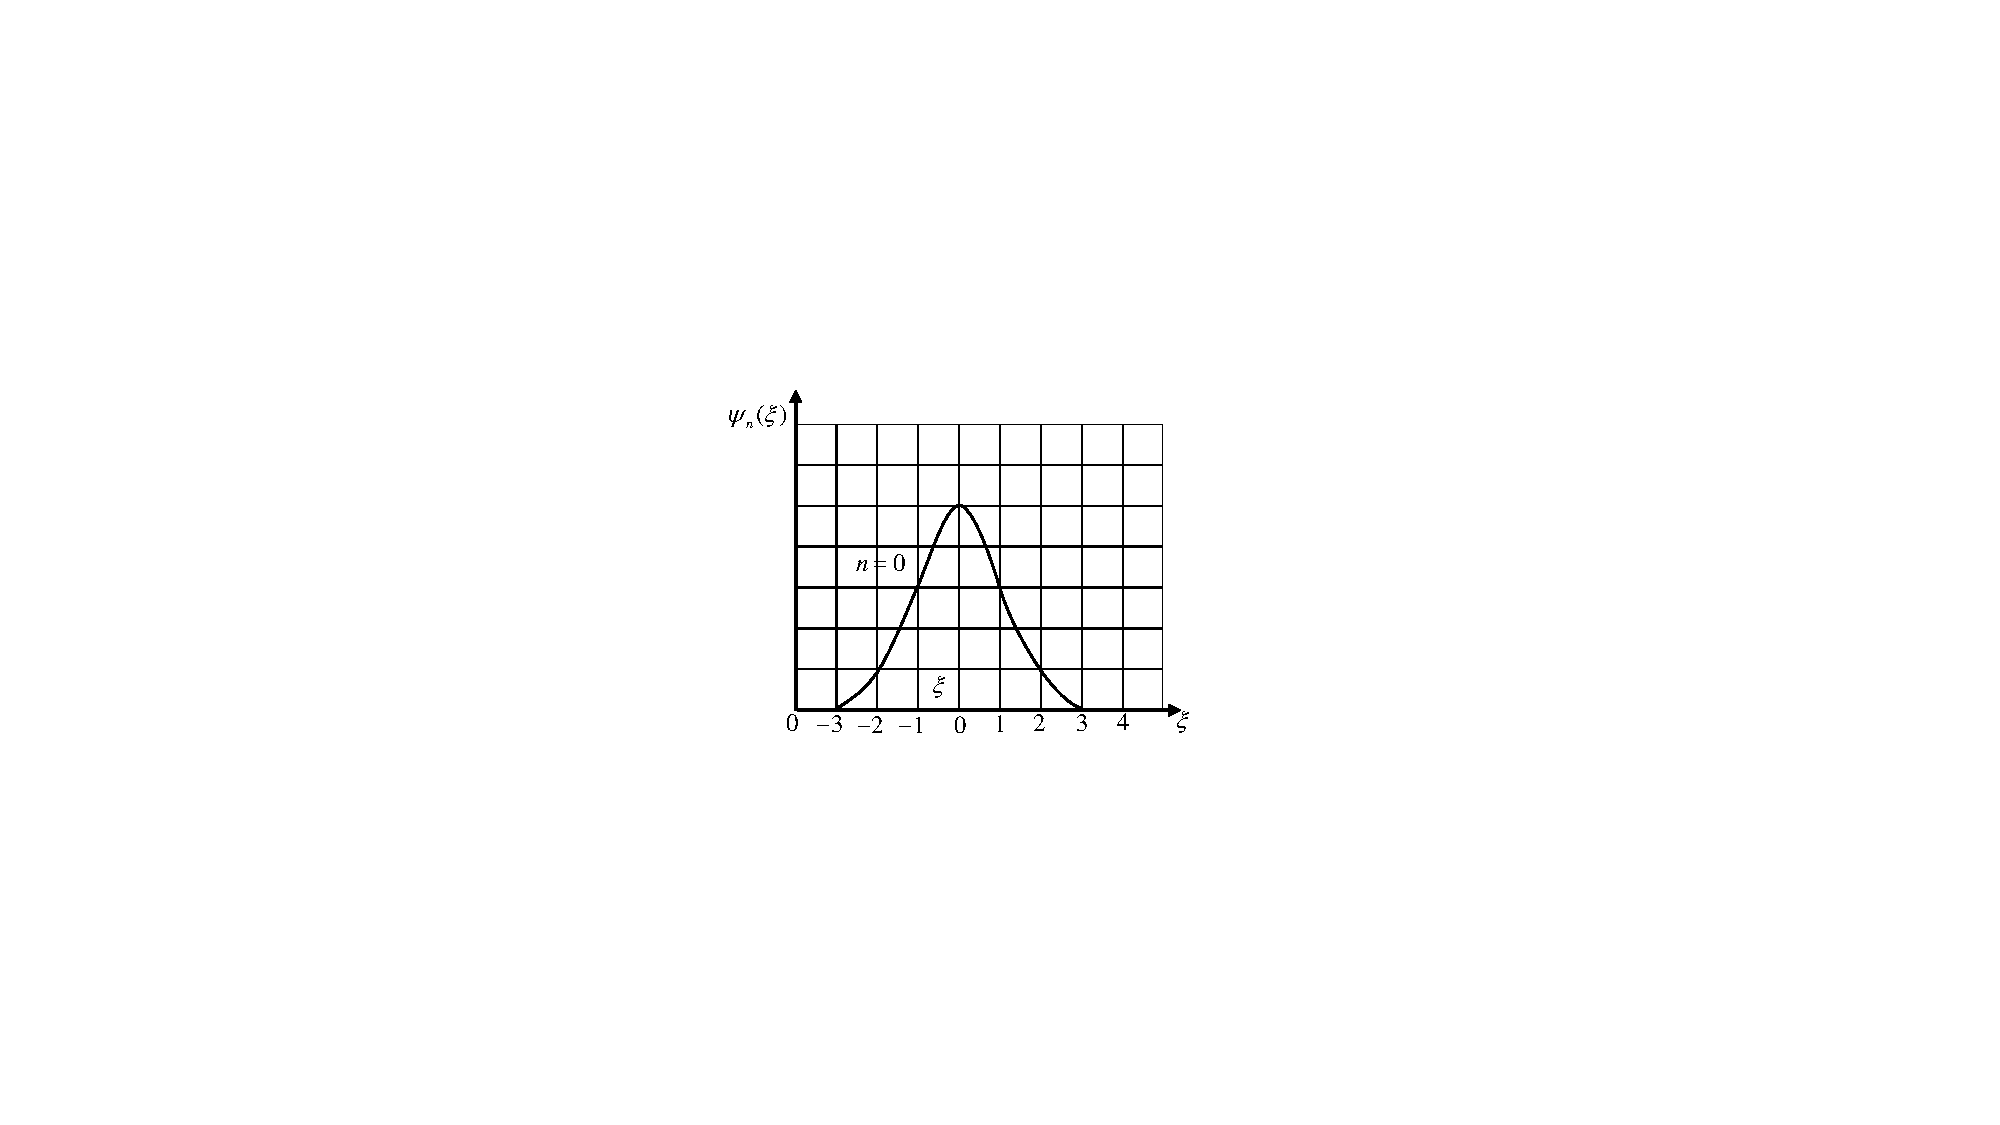
\includegraphics[width=0.6\linewidth]{QM file/figure/2-7(a)}
		%\centerline{(a)}
		\label{fig.2-7(a)}
	\end{minipage}
	\begin{minipage}[h]{0.49\linewidth}
		\centering
		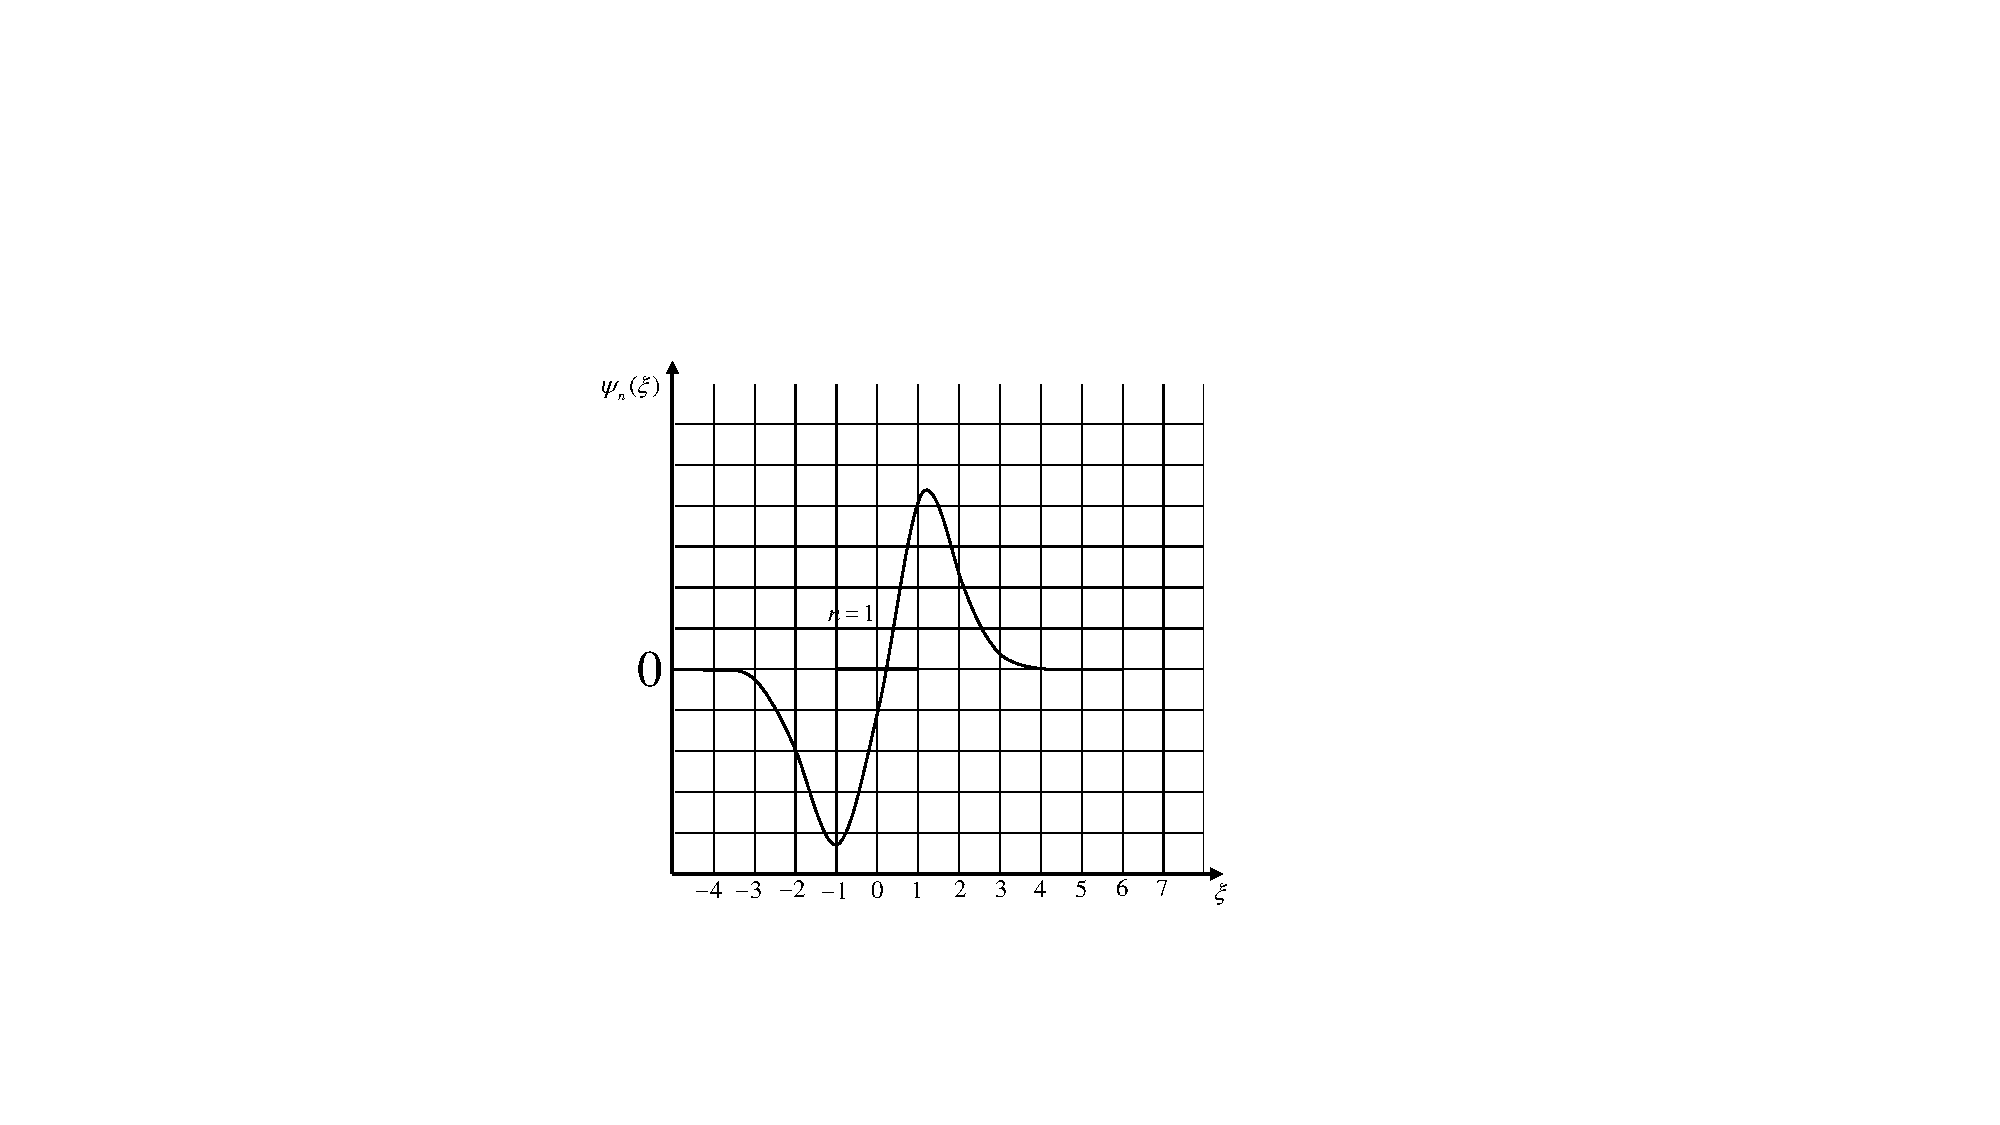
\includegraphics[width=0.6\linewidth]{QM file/figure/2-7(b)}
		%\centerline{(b)}
		\label{fig.2-7(b)}
	\end{minipage}%
	
	\begin{minipage}[h]{0.49\linewidth}
		\centering
		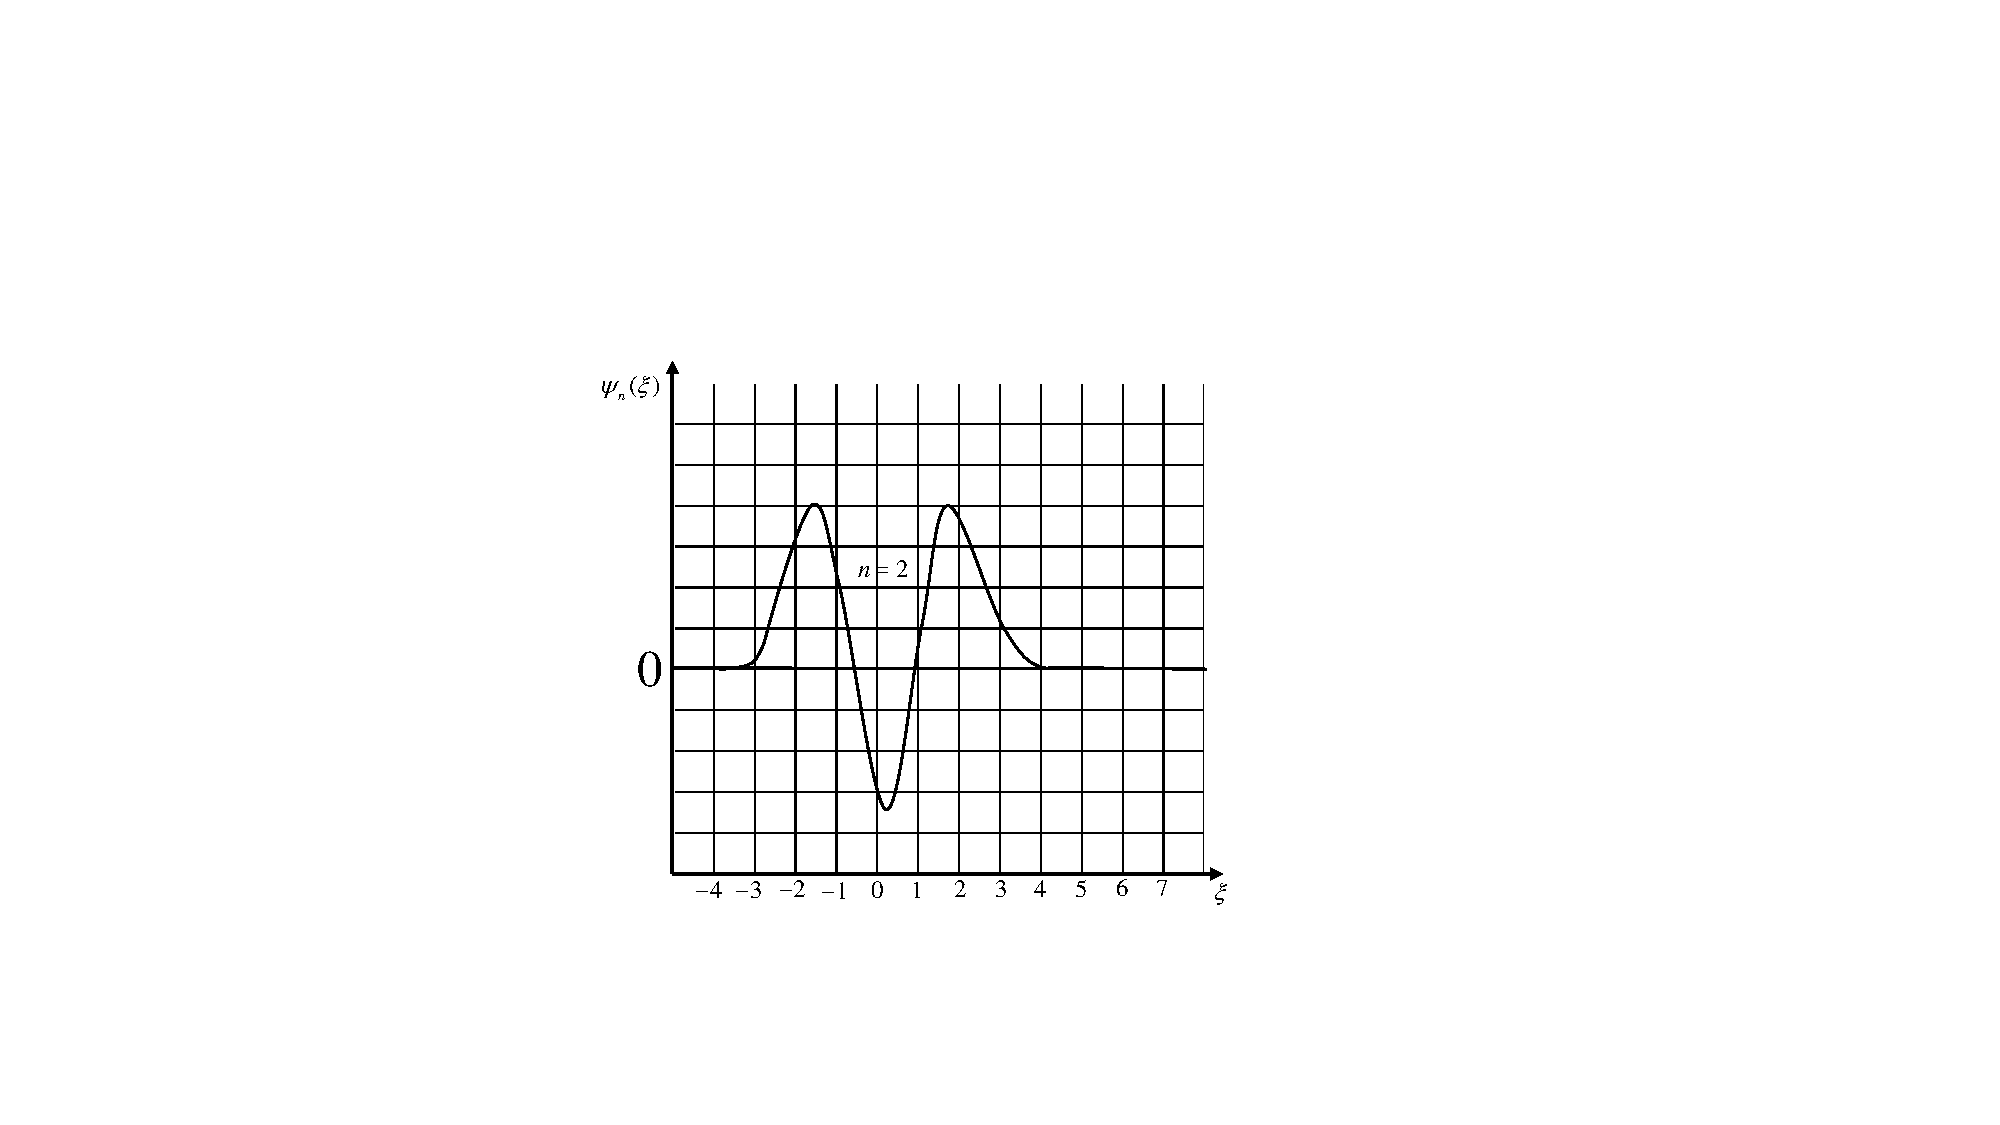
\includegraphics[width=0.6\linewidth]{QM file/figure/2-7(c)}
		%\centerline{(c)}
		\label{fig.2-7(c)}
	\end{minipage}
	\begin{minipage}[h]{0.49\linewidth}
		\centering
		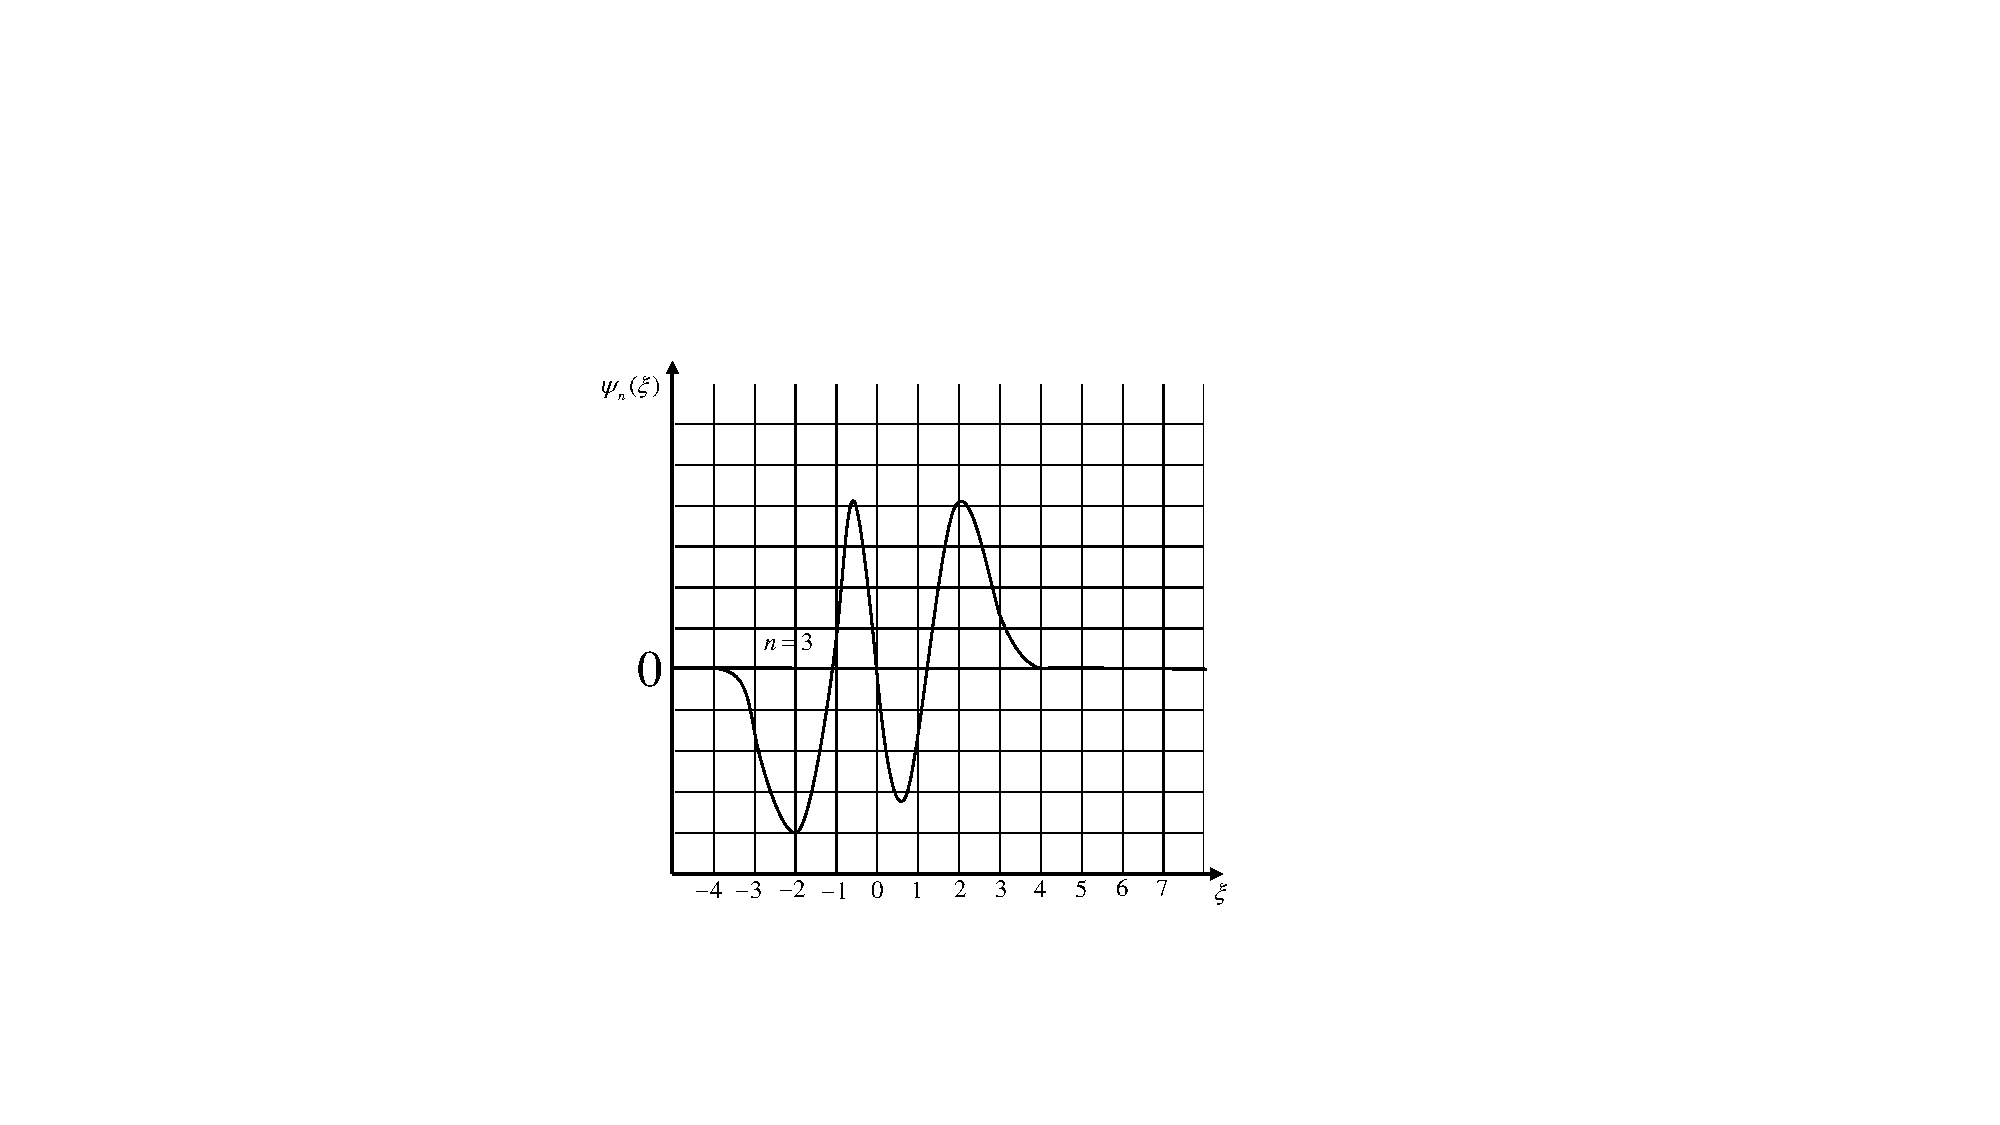
\includegraphics[width=0.6\linewidth]{QM file/figure/2-7(d)}
		%\centerline{(d)}
		\label{fig.2-7(d)}
	\end{minipage}
	\caption{}\label{fig.2-7}
\end{figure}
\begin{empheq}{equation*}
	E=\frac{1}{2}m(\pi v)^{2}A^{2}=2\times 10^{-12} \si{J}
\end{empheq}
而零点能仅为
\begin{empheq}{equation*}
	E_{0}=\frac{\hbar\omega}{2}=\frac{hv}{2}=3.3\times 10^{-34} \si{J}
\end{empheq}
完全不可能测量出来.

按照经典力学,能量为$E$的谐振子,所能达到的离平衡位置($x=0$)最远的距离是$|x|=A=\sqrt{\frac{2E}{m\omega^{2}}}$,$x=\pm A$称为谐振子的经典回转点,按照量子力学,当谐振子处于能量本征态$\varPsi_{n}$时,振子可在也$\varPsi_{n}\neq 0$的一切地点出现.例如,对于基态$\varPsi_{0}$,$E_{0}=\frac{\hbar\omega}{2}$,经典回转点为$|x|=\sqrt{\frac{\hbar}{m\omega}}=x_{0}$,振子在回转点以远(经典禁区)出现概率为
\begin{empheq}{equation}\label{eq25.20}
	2\int_{x_{0}}^{\infty}\varPsi_{0}^{2}dx=\frac{2}{\pi}\int_{1}^{\infty}e^{-\xi^{2}}d\xi=\num{0.1573}
\end{empheq}
对于第一激发态$\varPsi_{1}$,粒子在经典禁区出现的概率为\num{0.1116}.

在经典振幅以内($|x|<A$),量子力学给出的谐振子的空间分布概率也和经典力学结果显然不同.按照量子力学,振子在($x,x+dx$)内出现概率为$|\varPsi(x)|^{2}dx$,呈波浪起伏状.按照经典力学,振子通过($x,x+dx$)区间所用时间为$\frac{dx}{v}$,因此在这区间出现概率为
\setlength{\mathindent}{5em}
\begin{empheq}{equation}\label{eq25.21}
	\frac{\omega dx}{\pi v}=\frac{\omega dx}{\pi\sqrt{\frac{2(E-V)}{m}}}
	=\frac{\sqrt{m}\omega dx}{\pi\sqrt{2E-m\omega^{2}x^{2}}}=\boldsymbol{P}(x)dx
\end{empheq}\eqnormal
$x=0$;$\boldsymbol{P}(x)$为极小;$x\rightarrow\pm A$,$\boldsymbol{P}(x)\rightarrow\infty$.图 \ref{fig.2-8}(a)给出基态$\varPsi_{0}$的量子力学分布概率与经典力学分布概率的对比,两条分布曲线的形状刚好相反.但是,可以证明,当量子数$n$很大时,量子力学概率密度$|\varPsi_{n}(x)|^{2}$的局部平均与经典概率分布$\boldsymbol{P}(x)$趋于一致(对应原理),如图\ref{fig.2-8}(b)所示.
\begin{figure}[!h]
	\centering
		\begin{minipage}{0.49\linewidth}
			\centering
			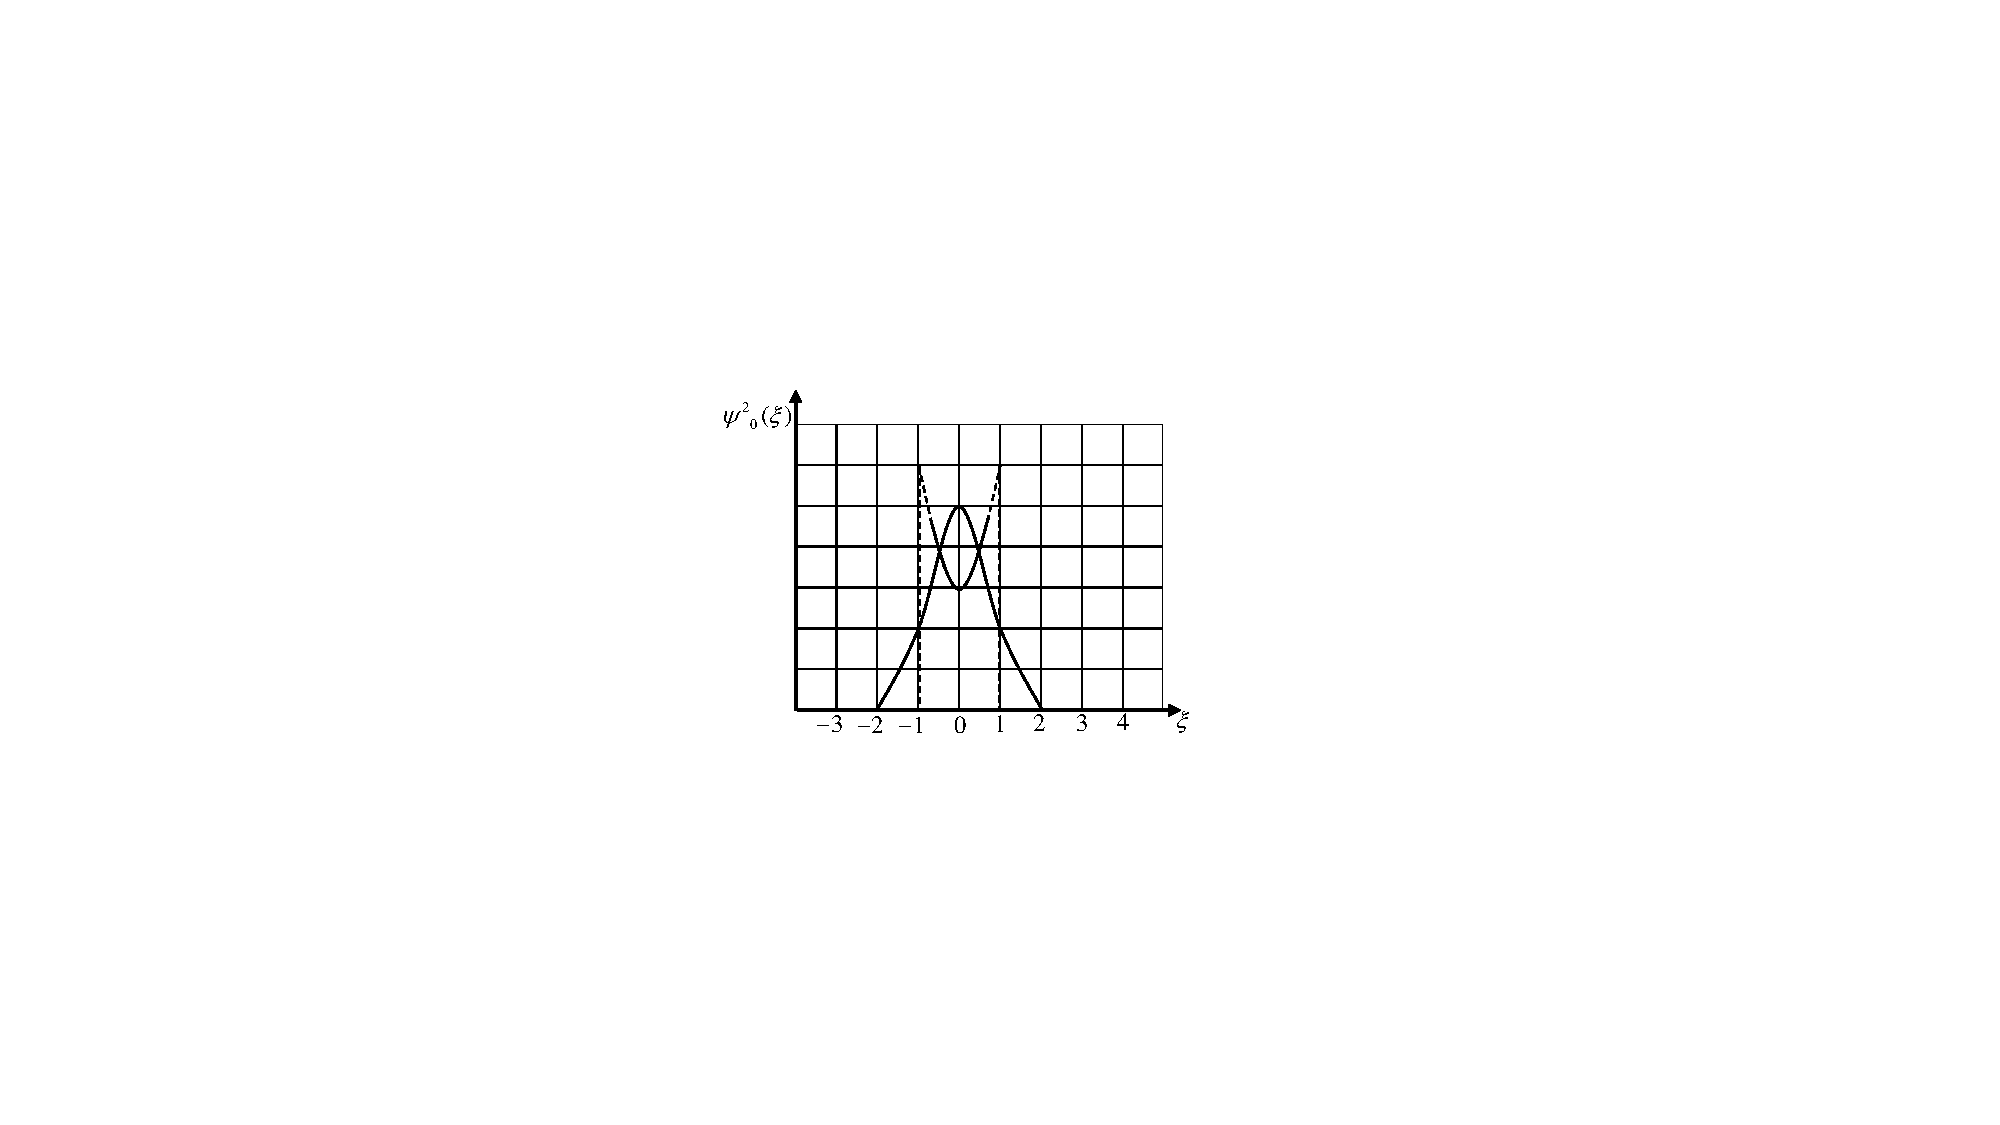
\includegraphics[width=0.7\linewidth]{QM file/figure/2-8(a)}
			\centerline{(a)}
			\label{fig.2-8a}%文中引用该图片代号
		\end{minipage}
		\begin{minipage}{0.49\linewidth}
			\centering
			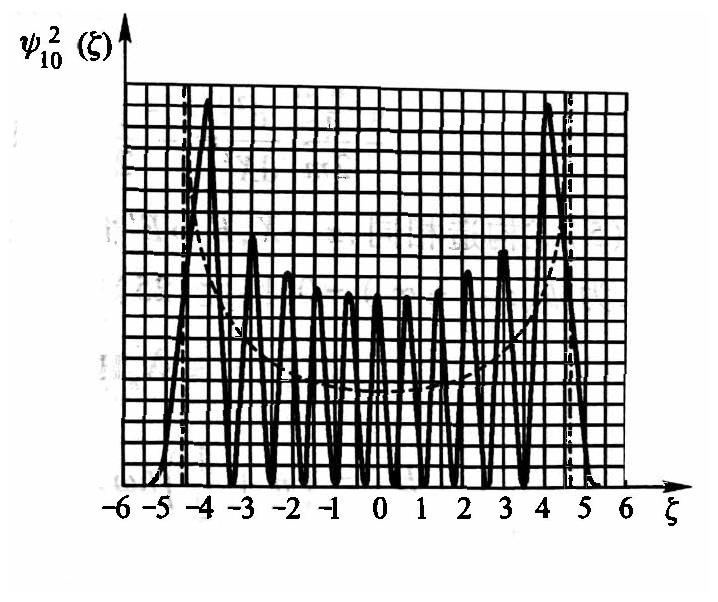
\includegraphics[width=0.7\linewidth]{QM file/figure/2-8(b)}
			\centerline{(b)}
			\label{fig.2-8b}%文中引用该图片代号
		\end{minipage}
	\caption{}\label{fig.2-8}
\end{figure}

图中虚线为经典分布概率曲线.

谐振子的波函数$\varPsi_{n}$相当典型地反映出束缚态波函数的一般特点.在经典允许区($E>V$),$\varPsi^{\prime\prime}$和$\varPsi$异号[参看\eqref{eq25.5}式] ,所以$x-\varPsi$曲线呈波形.在经典回转点,$E=V$,$\varPsi^{\prime\prime}=0$,是$x-\varPsi$曲线的最远的拐点(其他拐点是$\varPsi(x)$的节点).在经典禁区($E<V$),$\varPsi^{\prime\prime}$和$\varPsi$同号,二者随$|x|$的增大而一起衰减为0(波动消失).$\varPsi$开始衰减前的最后一个极大值出现在经典允许区内、经典回转点附近[参看图\ref{fig.2-8}(b)].

\example 质量$m$,电荷$q$的粒子,受到弹性力($-kx$)和均匀电场$\mathscr{E}$(沿正$x$轴方向)的共同作用,势能可以表示为
\begin{empheq}{equation}\label{eq25.22}
	V(x)=\frac{1}{2}kx^{2}-q\mathscr{E}x
\end{empheq}
求定态能级和波函数.

\solution $V(x)$可以表示成下列形式:
\eqlong
\begin{empheq}{equation*}
	V(x)=\frac{k}{2}\bigg(x^{2}-\frac{2q\mathscr{E}}{k}x\bigg)=\frac{k}{2}\bigg(x-\frac{q\mathscr{E}}{k}\bigg)^{2}-\frac{q^{2}\mathscr{E}^{2}}{2k}
\end{empheq}
令$k=m\omega^{2}$,则
\begin{empheq}{equation*}\label{eq25.22'}
	V(x)=\frac{1}{2}m\omega^{2}\bigg(x-\frac{q\mathscr{E}}{m\omega^{2}}\bigg)^{2}-\frac{q^{2}\mathscr{E}^{2}}{2m\omega^{2}}
\end{empheq}
再令
\begin{empheq}{equation}\label{eq25.23}
	X=x-\frac{q\mathscr{E}}{m\omega^{2}},\quad E^{\prime}=E+\frac{q^{2}\mathscr{E}^{2}}{2m\omega^{2}}
\end{empheq}
哈密顿算符可以表示为
\begin{empheq}{equation}\label{eq25.24}
	H=-\frac{\hbar^{2}}{2m}\frac{d^{2}}{dX^{2}}+\frac{1}{2}m\omega^{2}X^{2}-\frac{q^{2}\mathscr{E}^{2}}{2m\omega^{2}}
\end{empheq}
能量本征方程为
\begin{empheq}{equation}\label{eq25.25}
	-\frac{\hbar^{2}}{2m}\frac{d^{2}}{dX^{2}}\varPsi+\frac{1}{2}m\omega^{2}X^{2}\varPsi=E^{\prime}\varPsi
\end{empheq}\eqnormal
\eqref{eq25.25}式与\eqref{eq25.5}式构造相同,$x\rightarrow X$,$E\rightarrow E^{\prime}$而已.无限远处$\varPsi$的边条件也和没有电场时相同,为$\varPsi(x\rightarrow\pm\infty)=0$,因此\eqref{eq25.25}式的特征解必然是
\begin{empheq}{equation}\label{eq25.26}
	\varPsi_{n}(X)=N^{n}H^{n}\bigg(\frac{X}{x_{0}}\bigg)e^{-X^{2}/2x_{0}^{2}}
\end{empheq}
\begin{empheq}{equation}\label{eq25.27}
	E_{n}^{\prime}=\bigg(n+\frac{1}{2}\bigg)\hbar\omega
\end{empheq}
\eqref{eq25.26}式相当于\eqref{eq25.15}式中$x\rightarrow X$.由\eqref{eq25.23}、\eqref{eq25.27}式即得能级为
\eqlong
\begin{empheq}{equation}\label{eq25.28}
	E_{n}=E_{n}^{\prime}-\frac{q^{2}\mathscr{E}^{2}}{2m\omega^{2}}=\bigg(n+\frac{1}{2}\bigg)\hbar\omega-\frac{q^{2}\mathscr{E}}{2m\omega^{2}}
\end{empheq}\eqnormal
总之,电场$E$造成的效果是,各个能级均降低$\frac{q^{2}\mathscr{E}^{2}}{2m\omega^{2}}$,$\varPsi$中$x\rightarrow X$.因此粒子的平衡位置由$x=0$移至$X=0$,即$x=\frac{q\mathscr{E}}{m\omega^{2}}$.亦即粒子的状态向正$x$轴方向平移了距离$\frac{q\mathscr{E}}{m\omega^{2}}$.


% 势垒贯穿
\section[势垒贯穿]{势垒贯穿} \label{sec:02.06} % 
% \makebox[5em][s]{} % 短题目拉间距

设质量为$m$的粒子以给定的能量$E=\frac{\hbar^{2}k^{2}}{2m}$自左方入射,遇到图\ref{fig.2-9}所示的势垒:
\begin{equation}\label{eq26.1}
	V(x)=
	\begin{dcases}
		0, 		& x<0,x>a	\\
		V_{0},  & 0\leqslant x \leqslant a
	\end{dcases}
\end{equation}
设$V_{0}>E$,求粒子的运动状态.

\begin{wrapfigure}[9]{r}{8em}
	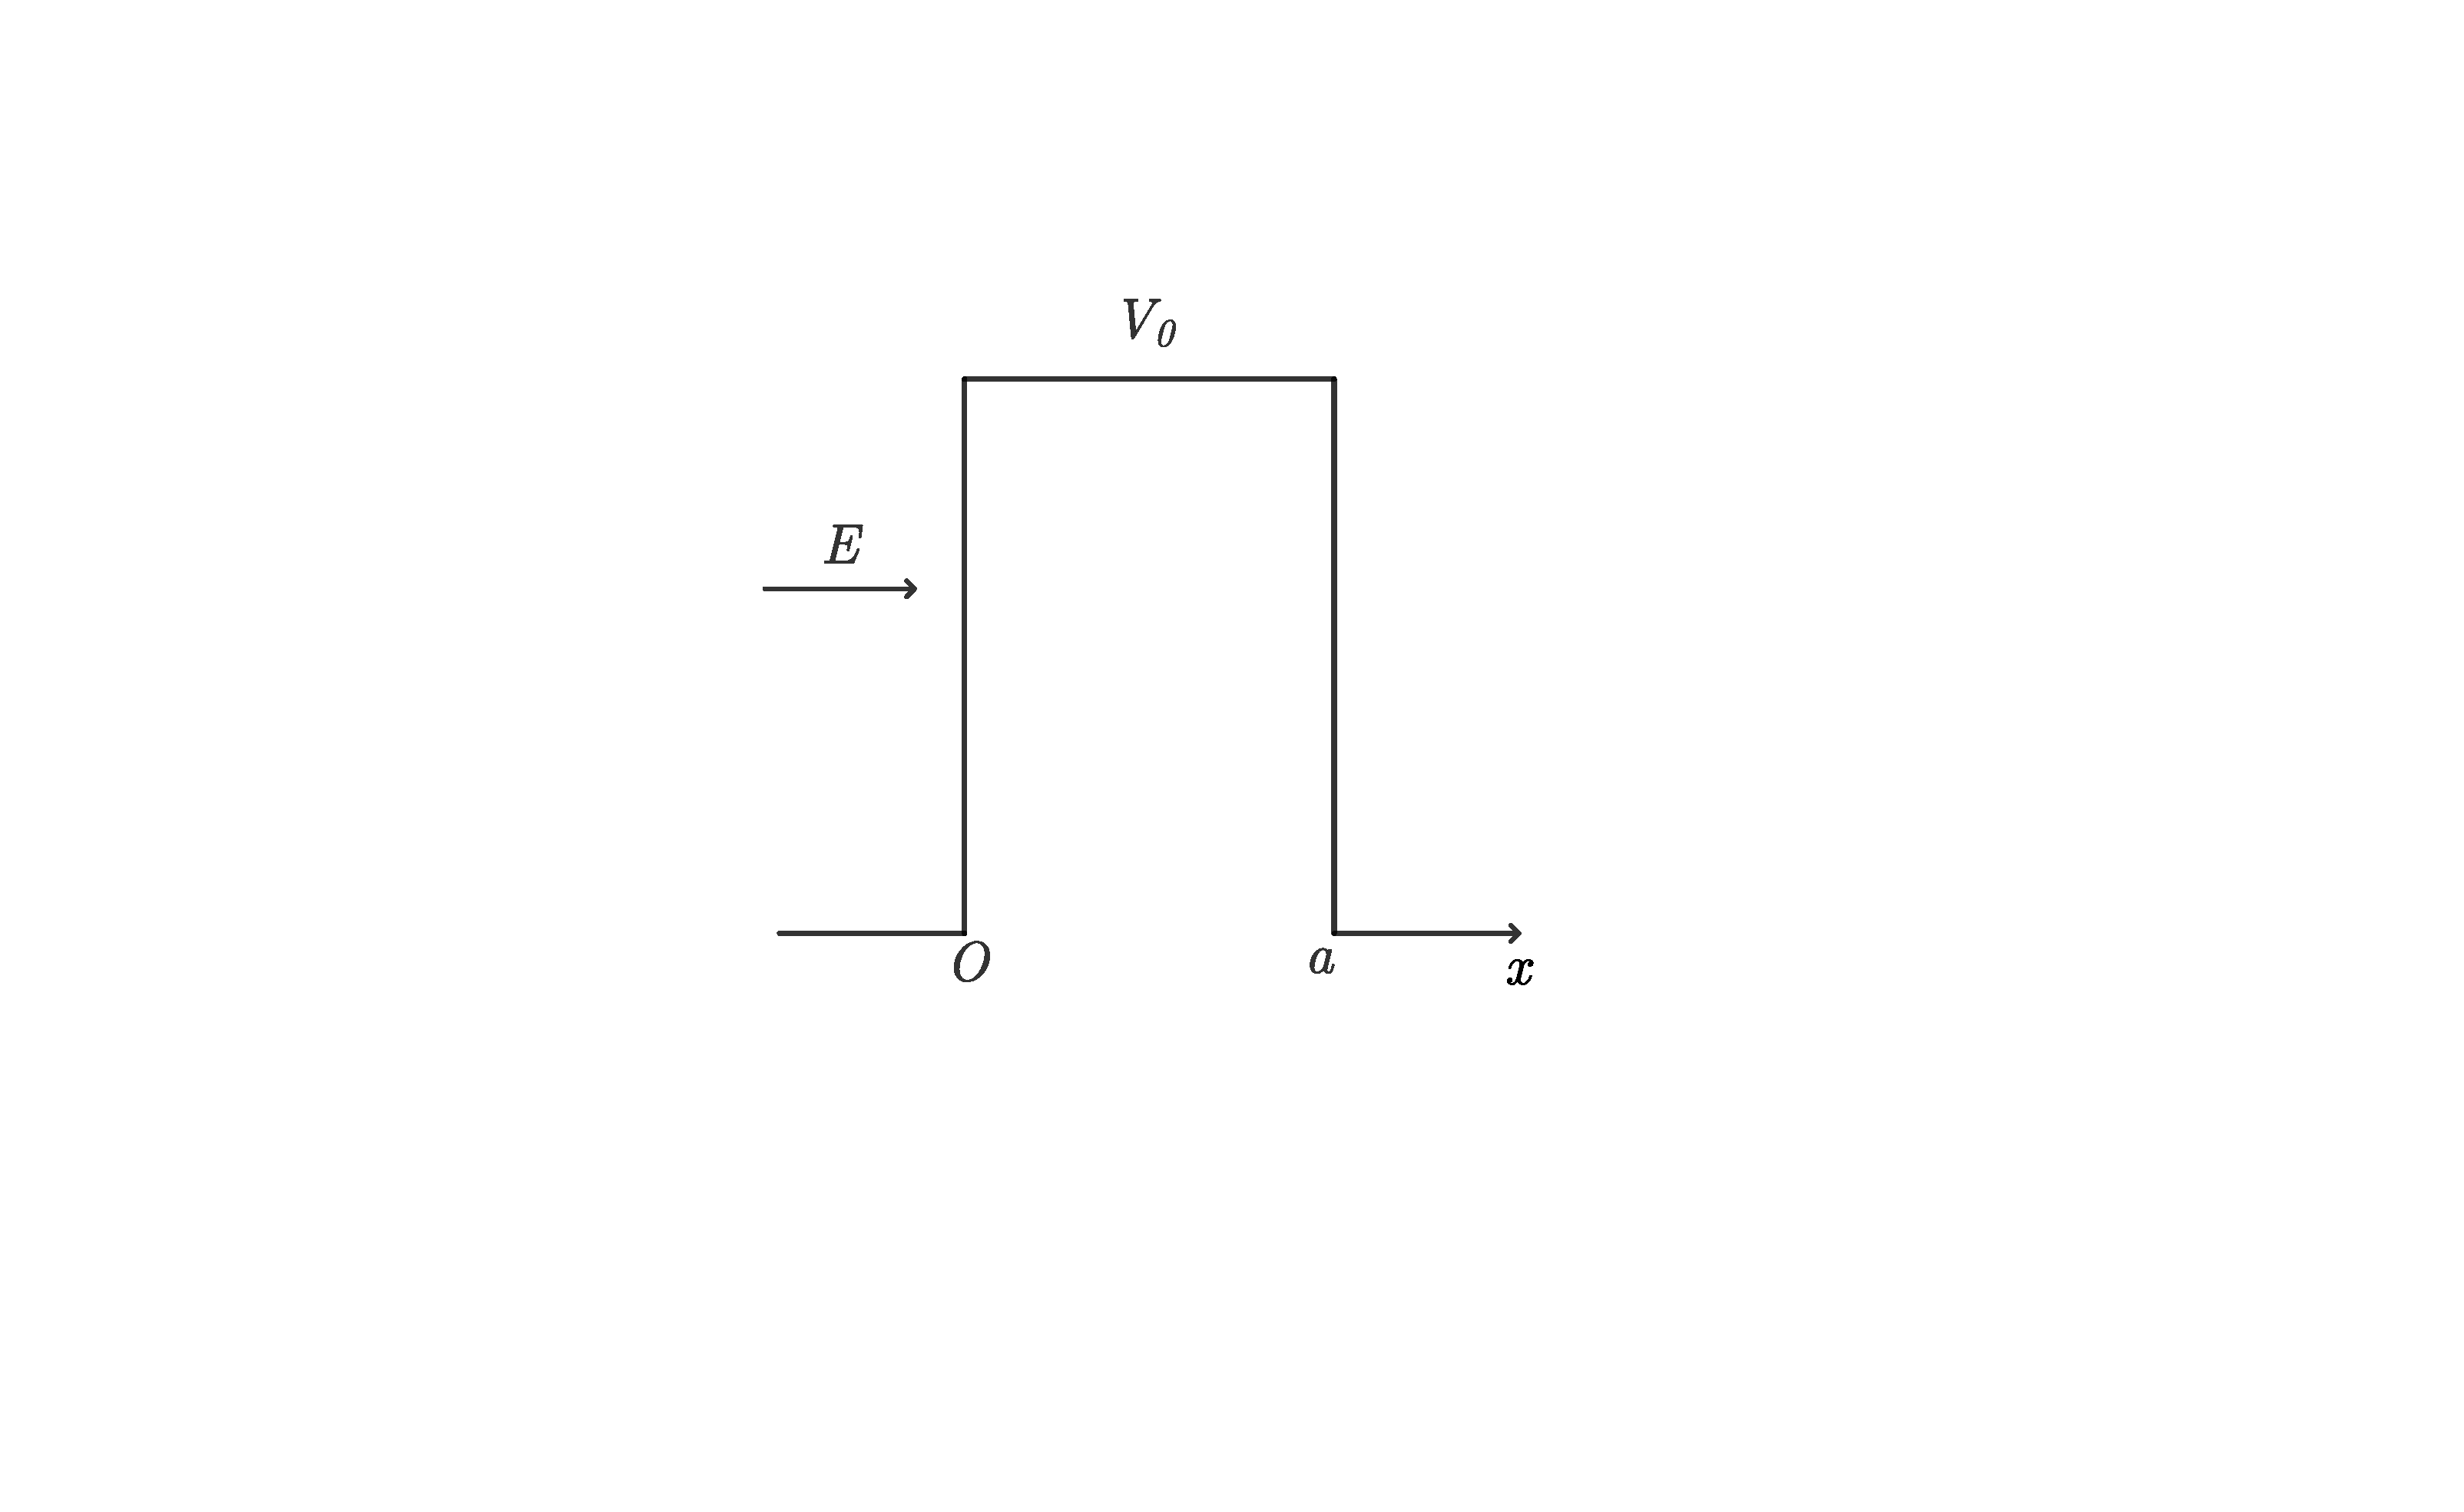
\includegraphics[width=3cm]{QM file/figure/2-9}
	\caption{}\label{fig.2-9}
\end{wrapfigure}

如果是经典力学问题,由于$V_{0}>E$,粒子不能越过势垒,将在$x=0$处被势垒反弹回去.作为量子力学问题,由于粒子的波动性,结论就不一样,可以证明,粒子将有一定概率透过势垒进入$x>a$区域而继续前进.由于粒子的能量是给定的,而且粒子是从$x=-\infty$处射来,这是一个属于游离态的定态问题,波函数可以表示成
\begin{empheq}{equation}\label{eq26.2}
	\varPsi(x,t)=\varPsi(x)e^{-iEt/\hbar}
\end{empheq}
空间波函数$\varPsi(x)$满足定态薛定谔方程:
\begin{empheq}{equation*}\label{eq26.3}
	-\frac{\hbar^{2}}{2m}\varPsi^{\prime\prime}+V(x)\varPsi=E\varPsi=\frac{\hbar^{2}k^{2}}{2m}\varPsi	\tag{2.6.3}
\end{empheq}
亦即
\begin{subnumcases}{}
	\varPsi^{\prime\prime}+k^{2}\varPsi=0,		& x<0,x>a	\label{eq26.3a}\\
	\varPsi^{\prime\prime}-\beta^{2}\varPsi=0,	& 0\leqslant x \leqslant a \label{eq26.3b}
\end{subnumcases}
其中
\begin{empheq}{equation}\label{eq26.4}
	k=\frac{\sqrt{2mE}}{\hbar},\quad \beta=\frac{\sqrt{2m(V_{0}-E)}}{\hbar}
\end{empheq}
\eqref{eq26.3a}式的解为$\varPsi\thicksim e^{\pm ikx}$,考虑到“粒子由左方入射”这个边条件,应取
\begin{subnumcases}{\varPsi(x)=}
	Ae^{ikx}+Re^{-ikx},		& x<0	\label{eq26.5a}\\
	De^{ikx},				& x>a	\label{eq26.5b}
\end{subnumcases}
$A$项为入射波,$R$项为反射波,$D$项为透射波.由于并无粒子从右方入射,所以$x>a$区域没有项$e^{-ikx}$.\eqref{eq26.3b}式的解为
\begin{empheq}{equation*}\label{eq26.5c}
	\varPsi(x)=Be^{\beta x}+Ce^{-\beta x},\quad 0<x<a	\tag{2.6.5c}
\end{empheq}
其中入射波振幅$ A $可以任意给定,其余4个系数可以利用$ x=0 $,a处$\varPsi$和$\varPsi^{\prime\prime}$的连续条件求出.按照\eqref{eq22.9}式及例题,容易求出
\setlength{\mathindent}{6em}
\begin{empheq}{align*}
	\text{入射流量}\quad j_{A}&=|A|^{2}\frac{\hbar k}{m}	\\
	\text{反射流量}\quad j_{R}&=|R|^{2}\bigg( -\frac{\hbar k}{m} \bigg) \\
	\text{透射流量}\quad j_{D}&=|D|^{2}\frac{\hbar k}{m}
\end{empheq}\eqnormal
因此粒子被势垒反射回去的概率(反射系数)和透过势垒的概率(透射系数)为
\begin{equation}\label{eq26.6}
	\begin{aligned}
		\text{反射系数}&=|\frac{j_{R}}{j_{A}}|=|\frac{R}{A}|^{2}	\\
		\text{透射系数}&=|\frac{j_{D}}{j_{A}}|=|\frac{D}{A}|^{2}
	\end{aligned}
\end{equation}
以下求系数$R,D$.$x=0$处$\varPsi(x)$及$\varPsi^{\prime}(x)$应该连续,由\eqref{eq26.5a},\eqref{eq26.5b}式易得
\begin{equation}\label{eq26.7}
	\begin{dcases}
		A+R=B+C	\\
		ik(A-R)=\beta(B-C)
	\end{dcases}
\end{equation}
$x=a$处$\varPsi$及$\varPsi^{\prime}$也应该连续,由\eqref{eq26.5b},\eqref{eq26.5c}式易得
\begin{equation}\label{eq26.8}
	\begin{dcases}
		De^{ika}=Be^{\beta a}+Ce^{-\beta a}	\\
		ikDe^{ika}=\beta Be^{\beta a}-\beta Ce^{-\beta a}
	\end{dcases}
\end{equation}
由\eqref{eq26.7}式可得
\begin{equation}\label{eq26.9}
	\begin{cases}
		\frac{2B}{A}=1+\frac{ik}{\beta}+\bigg(1-\frac{ik}{\beta}\bigg)\frac{R}{A}		\\
		\frac{2C}{A}=1-\frac{ik}{\beta}+\bigg(1+\frac{ik}{\beta}\bigg)\frac{R}{A}	
	\end{cases}
\end{equation}
由(8)式可得
\begin{equation}\label{eq26.10}
	\begin{cases}
		\frac{2B}{A}=\bigg(1+\frac{ik}{\beta}\bigg)\frac{D}{A}e^{-\beta a+ika}		\\
		\frac{2C}{A}=\bigg(1-\frac{ik}{\beta}\bigg)\frac{D}{A}e^{\beta a+ika}	
	\end{cases}
\end{equation}
比较\eqref{eq26.9}、\eqref{eq26.10}式,得到
\begin{equation}\label{eq26.11}
	\begin{cases}
		\gamma+\frac{R}{A}=\frac{D}{A}\gamma e^{-\beta a+ika}		\\
		\gamma^{*}+\frac{R}{A}=\frac{D}{A}\gamma^{*}e^{\beta a+ika}	
	\end{cases}
\end{equation}
其中
\setlength{\mathindent}{5em}
\begin{empheq}{equation}\label{eq26.12}
	\gamma=\frac{\beta+ik}{\beta-ik},\quad \gamma^{*}=\frac{\beta-ik}{\beta+ik}=\frac{1}{\gamma},\quad |\gamma|=1
\end{empheq}
由\eqref{eq26.11}式解出
\begin{empheq}{equation}\label{eq26.13}
	\frac{D}{A}=\frac{(\gamma-\gamma^{*})e^{-ika}}{\gamma e^{-\beta a}-\gamma^{*}e^{\beta a}},\quad
	\frac{R}{A}=\frac{e^{\beta a}-e^{-\beta A}}{\gamma e^{-\beta a}-\gamma^{*}e^{\beta a}}
\end{empheq}
\begin{equation}\label{eq26.14}
	\begin{aligned}
		|\frac{D}{A}|^{2} &=\frac{(\gamma-\gamma^{*})^{2}}{e^{2\beta a}+e^{-2\beta a}-(\gamma^{2}+\gamma^{*2})}	\text{(透射系数)}	\\
		|\frac{R}{A}|^{2} &=\frac{(e^{\beta a}-e^{-\beta a})^{2}}{e^{2\beta a}+e^{-2\beta a}-(\gamma^{2}+\gamma^{*2})}	\text{(反射系数)}
	\end{aligned}
\end{equation}
\eqnormal
利用关系式
\begin{empheq}{equation*}
	|\gamma-\gamma^{*}|^{2}=2-(\gamma^{2}+\gamma^{*2})
\end{empheq}
容易证明
\begin{empheq}{equation}\label{eq26.15}
	|\frac{D}{A}|^{2}+|\frac{R}{A}|^{2}=1
\end{empheq}
这是概率守恒的具体表现形式.

在许多问题中,$e^{2\beta a}\gg 1$,这时\eqref{eq26.14}式分母可以近似取为$e^{2\beta a}$,从而得到
\setlength{\mathindent}{4em}
\begin{empheq}{equation}\label{eq26.16}
	|\frac{D}{A}|^{2}\approx|\gamma-\gamma^{*}|^{2}e^{-2\beta a}
	=\frac{16E(V_{0}-E)}{V_{0}^{2}}e^{-\frac{2a}{\hbar}\sqrt{2m(V_{0}-E)}}
\end{empheq}\eqnormal
这就是$E<V_{0}$时矩形势垒穿透系数的常用公式.为了获得明确的量级概念,举两个简单的例子.

1. 宏观情形,取$m=1\si{g},V_{0}-E=10^{-7}\si{J},a=1\si{cm}$,则
\begin{empheq}{gather*}
	\frac{2a}{\hbar}\sqrt{2m(V_{0}-E)}=\num{2.68}\times10^{27}	\\
	|\frac{D}{A}|^{2}\thicksim e^{-2.68\times10^{27}}\thicksim10^{-1.16\times10^{27}}
\end{empheq}
真是微乎其微!宏观领域从未发现势垒贯穿现象,就是因为概率太小.

2. 微观情形,取$m=m_{e}\text{(电子质量)},V_{0}-E=1\si{eV},a=0.1\si{nm}$,则
\begin{empheq}{gather*}
	\frac{2a}{\hbar}\sqrt{2m(V_{0}-E)}=\num{1.026}	\\
	|\frac{D}{A}|^{2}\thicksim e^{-\frac{2a}{\hbar}\sqrt{2m(V_{0}-E)}}\thicksim e^{-1.026}=\num{0.36}
\end{empheq}
透射概率相当大,由此可见在微观领域势垒贯穿现象是容易发生的.

到\eqref{eq26.15}式为止的结果是严格的,而且不难推广到$E>V_{0}$的情况(包括$V_{0}<0$,即势阱的情况).这种情况下的结果,和光波在折射率不同的几层介质中的传播规律(反射,透射)类似.

当$E>V_{0}$,\eqref{eq26.4}式中$\beta$为虚数,
\begin{empheq}{equation*}\label{eq26.4'}
	\beta=\frac{\sqrt{2m(V_{0}-E)}}{\hbar}=\frac{i\sqrt{E-V_{0}}}{\hbar}=i\alpha	\tag{$2.6.4^{\prime}$}
\end{empheq}
代入\eqref{eq26.12}式
\begin{empheq}{equation*}\label{eq26.12'}
	\gamma=\frac{\alpha+k}{\alpha-k},\quad \gamma^{*}=\frac{\alpha-k}{\alpha+k},\quad 
	\gamma\gamma^{*}=1	\tag{$2.6.12^{\prime}$}
\end{empheq}
\eqref{eq26.13}、\eqref{eq26.14}式中
\setlength{\mathindent}{5em}
\begin{empheq}{equation}\label{eq26.17}
	\begin{aligned}
		e^{\beta a}=e^{-\alpha a},&\quad e^{-\beta a}=e^{-i\alpha a}	\\
		(\gamma-\gamma^{*})^{2}=\bigg(\frac{4\alpha k}{\alpha^{2}-k^{2}}\bigg)^{2},&
		\gamma^{2}+\gamma^{*2}=2+\bigg(\frac{4\alpha k}{\alpha^{2}-k^{2}}\bigg)^{2}
	\end{aligned}
\end{empheq}\eqnormal
在一般情况下,$\alpha,k$量级相同,\eqref{eq26.14}式分子、分母中各项量级也相同,所以反射系数$|\frac{R}{A}|^{2}$与透射系数$|\frac{D}{A}|^{2}$的量级也大致相同,透射很容易.

有一种特殊情况值得注意,如果$e^{i\alpha a}=e^{-i\alpha a}$,即
\begin{empheq}{equation}\label{eq26.18}
	e^{i2\alpha a}=1,\quad \alpha a=\pi,2\pi,3\pi,\cdots
\end{empheq}
由\eqref{eq26.14}式可以看出$R=0$,没有反射,而透射系数$|\frac{D}{A}|^{2}=1$.这种情形称为共振透射.共振条件\eqref{eq26.18}也就是
\setlength{\mathindent}{5em}
\begin{empheq}{equation}\label{eq26.19}
	\frac{2a}{\lambda}=1,2,3,\cdots,\quad \lambda=\frac{2\pi}{\alpha}=\frac{h}{\sqrt{2m(E-V_{0})}}
\end{empheq}\eqnormal
$\lambda$为粒子在势垒(阱)内的物质波波长.

对于一般形状的势垒(见图\ref{fig.2-10}),透射系数的计算较复杂(求解定态薛定谔方程!)但如入射能量$E$较小,$V(x)>E$的区域相当宽,总透射系数很小,则可以用以下的粗略近似处理.

\begin{wrapfigure}[9]{r}{12em}
	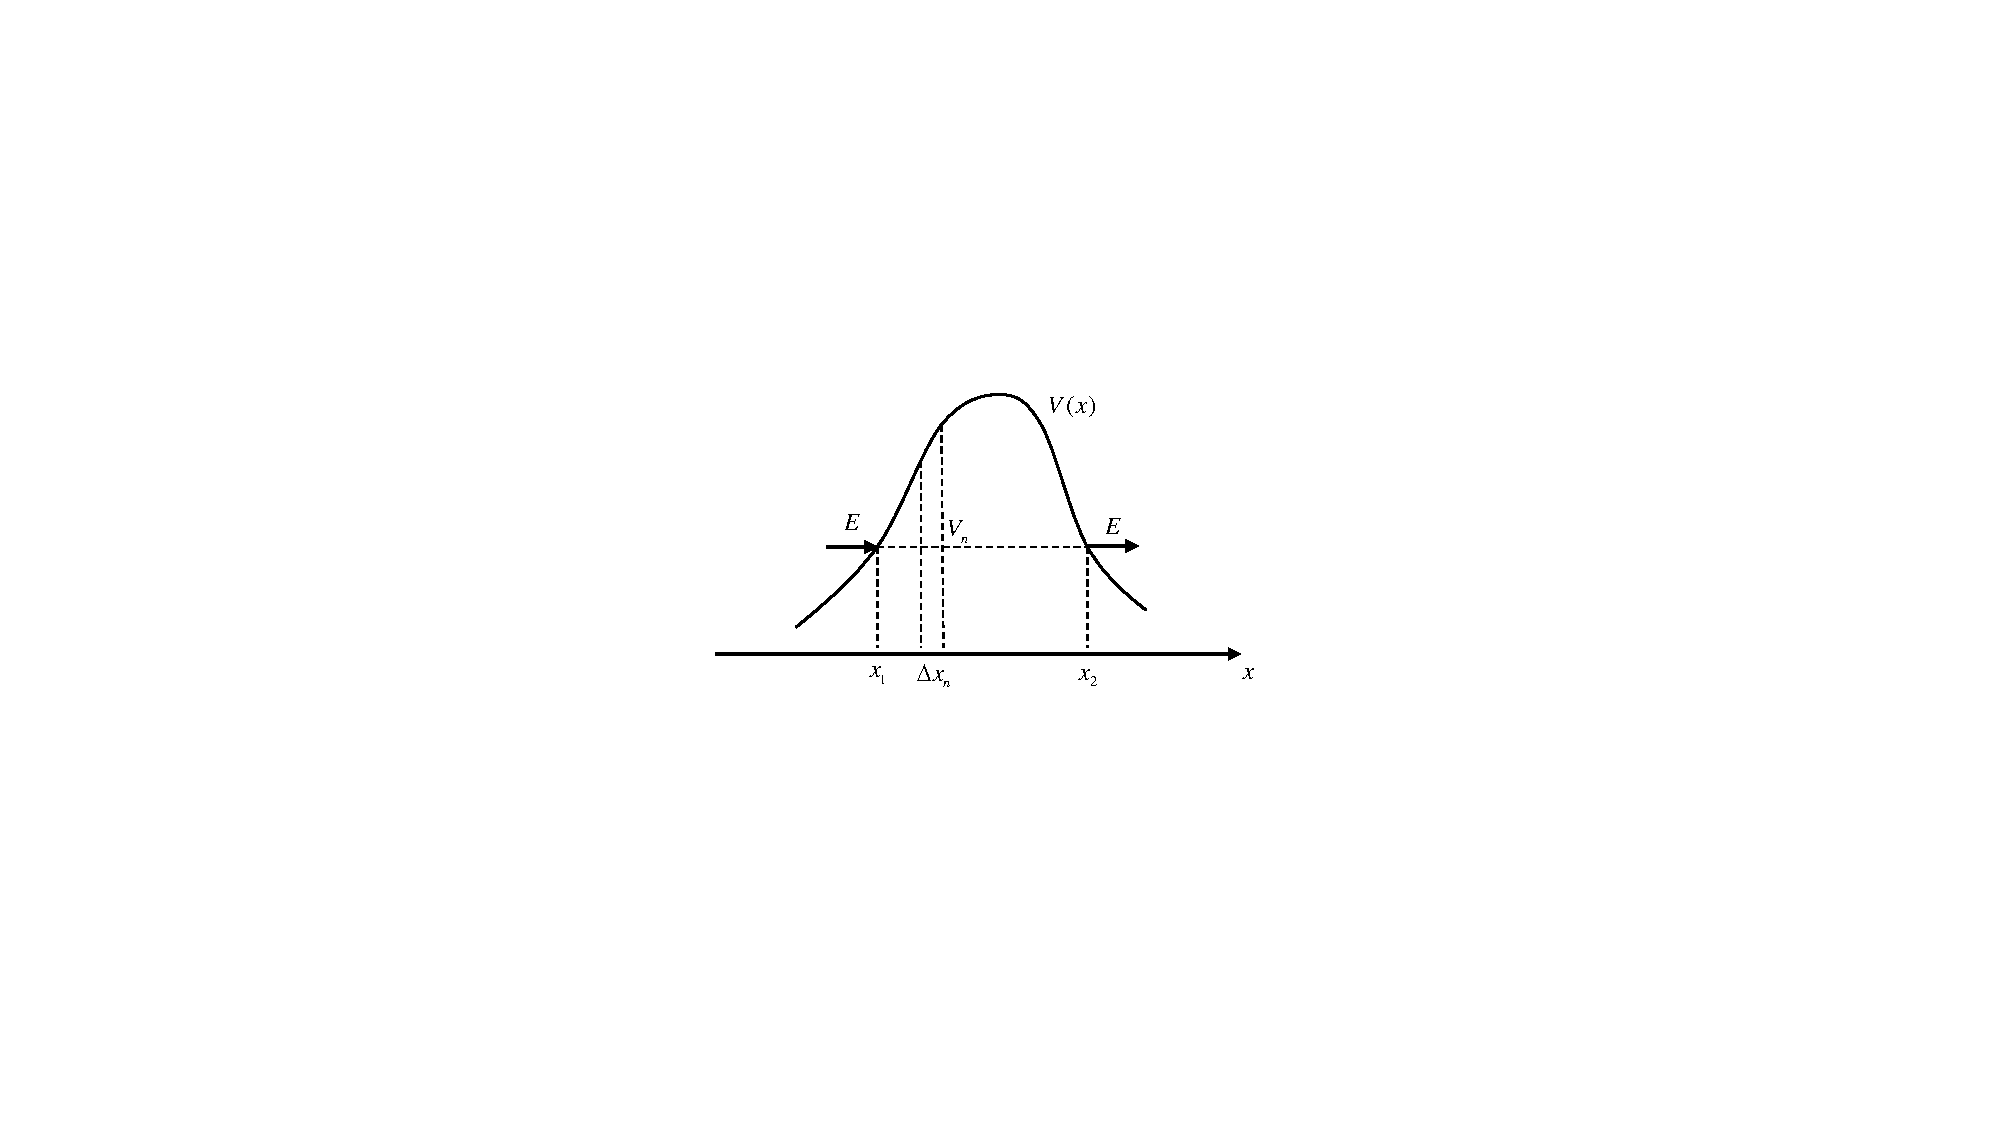
\includegraphics[width=4cm]{QM file/figure/2-10}
	\caption{}\label{fig.2-10}
\end{wrapfigure}

将$V(x)>E$的部分划分成许多窄条(宽$\Delta x_{n}$)状的矩形势垒,粒子对其中一条的穿透概率取为
\setlength{\mathindent}{5em}
\begin{empheq}{equation*}
	e^{\frac{2\Delta x_{n}}{\hbar}\sqrt{2m(V_{0}-E)}}
\end{empheq}\eqnormal
各条穿透概率的乘积等于粒子对整个势垒的总穿透概率.($V<E$的部分,容易穿透,概率按1处理)因此
\setlength{\mathindent}{4em}
\begin{empheq}{equation}\label{eq26.20}
	\text{总穿透概率}\thicksim \exp\big[-\frac{2}{\hbar}\sqrt{2m}\int_{x_{1}}^{x^{2}}\sqrt{V(x)-E}dx\big]
\end{empheq}\eqnormal
$x_{1},x_{2}$为经典回转点,即$V(x_{1})=V(x_{2})=E$.

势垒贯穿现象也称“隧道效应”.诸如原子核的$\alpha$放射性,导体中自由电子的形成,不同导体间的接触电势差, 都与隧道效应有关.20 世纪60年代,利用电子在结型半导体中的隧道效应,制成了有名的隧道二极管.

\example 金属中自由电子的“冷发射”.

在金属表面加一个强电场($\mathscr{E}\thicksim10^{6}\si{V/cm}$)电子就能从金属中逸出,这现象称为冷发射[将金属(阴极)加热而得到电流,称为热发射].这是一种典型的隧道效应.

加外电场前,金属中自由电子所处平均势场大致如图\ref{fig.2-11}(a)所示,$x<0$为金属,$V\approx 0$,$x>0$为真空,$V\approx V_{0}$,$(V_{0}-E)$就是电子逸出金属所需能量(逸出功).由于势垒为半无限宽,电子无法逸出(穿透概率为0).以金属为阴极,加强电场$\mathscr{E}$后,势能变成
\begin{figure}[htbp]
	\centering
	\begin{minipage}{0.49\linewidth}
		\centering
		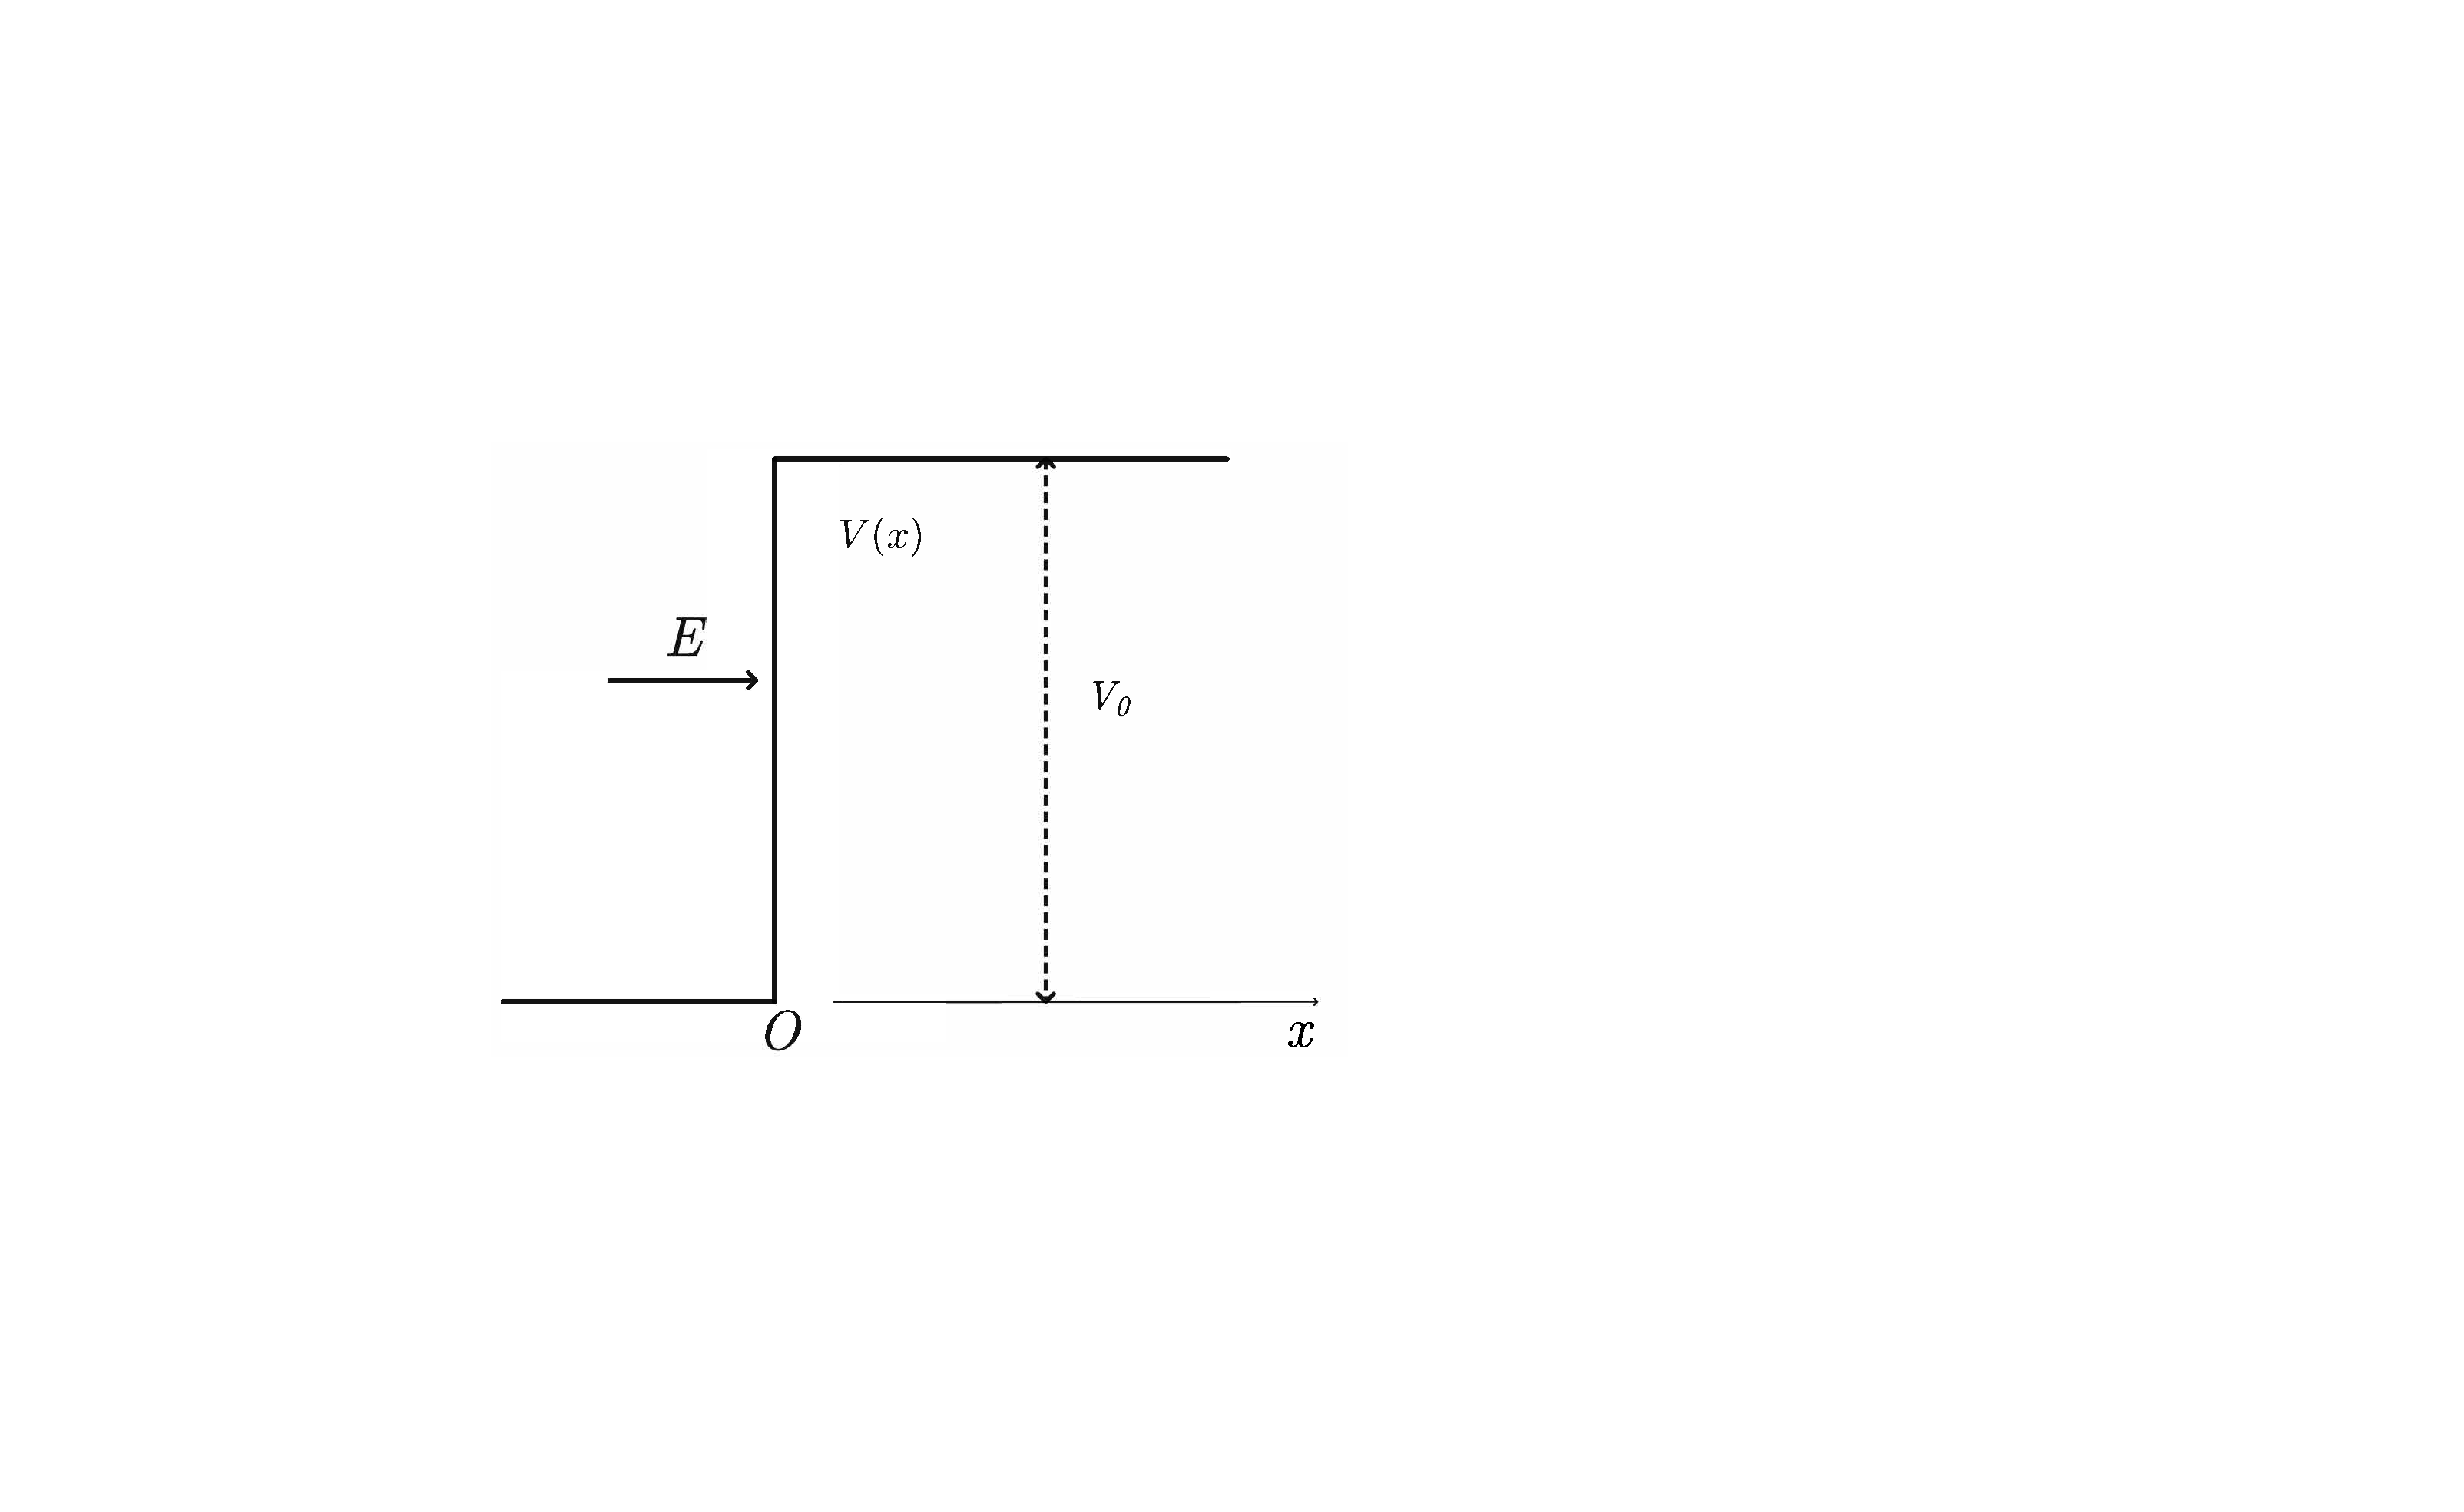
\includegraphics[width=0.6\linewidth]{QM file/figure/2-11(a)}
		\centerline{(a)}
		%\label{fig.2-11(a)}%文中引用该图片代号
	\end{minipage}
	\begin{minipage}{0.49\linewidth}
		\centering
		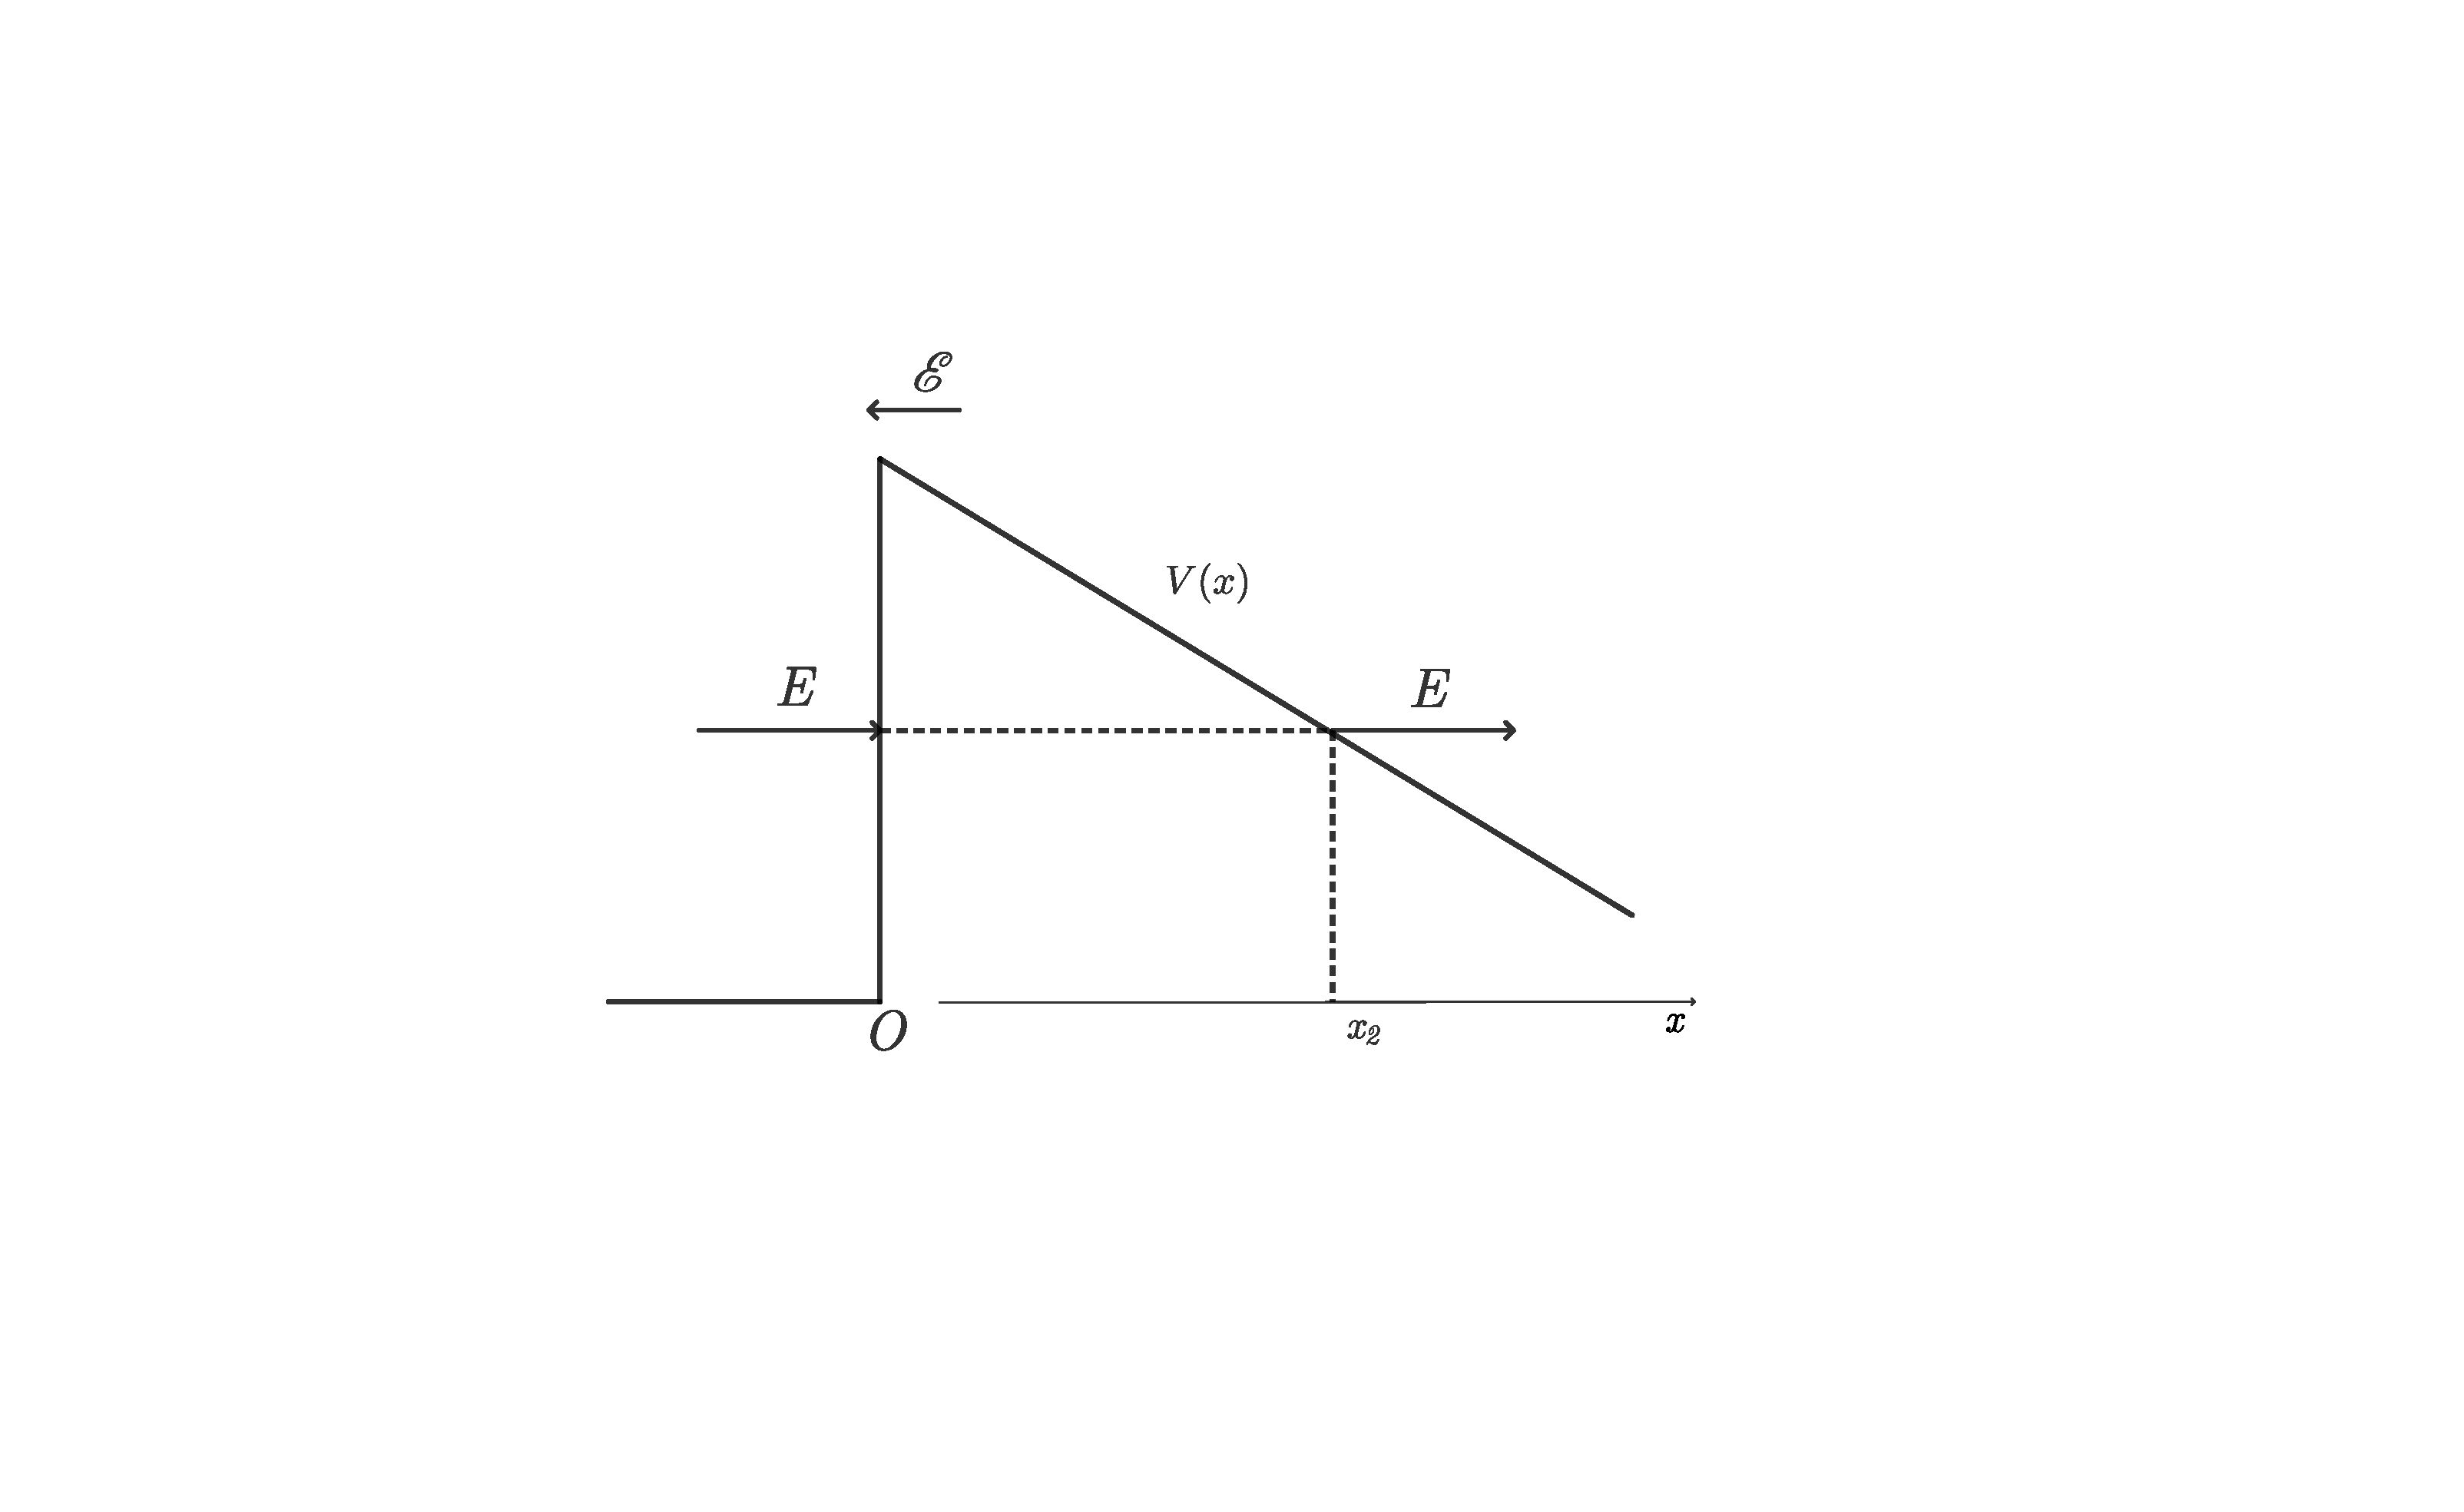
\includegraphics[width=0.6\linewidth]{QM file/figure/2-11(b)}
		\centerline{(b)}
		%\label{fig.2-11(b)}%文中引用该图片代号
	\end{minipage}
	\caption{}\label{fig.2-11}
\end{figure}
\begin{equation}\label{eq26.21}
	V(x)=
	\begin{dcases}
	0,		& x<0	\\	
	V_{0}-e\mathscr{E}x,	& x>0	
	\end{dcases}
\end{equation}
形成图\ref{fig.2-11}(b)所示的三角形势垒按照\eqref{eq26.20}式,电子对势垒的穿透概率约为
\setlength{\mathindent}{5em}
\begin{empheq}{equation}\label{eq26.22}
	exp\big[-\frac{2}{\hbar}\sqrt{2m}\int_{0}^{x^{2}}\sqrt{2m(V_{0}-E-e\mathscr{E}x)}dx\big]
	=e^{-\bar{\mathscr{E}_{0}}/\mathscr{E}}
\end{empheq}
其中
\begin{empheq}{equation}\label{eq26.23}
	x=\frac{(V_{0}-E)}{e\mathscr{E}},\quad \mathscr{E}_{0}=\frac{4}{3e\hbar}=\sqrt{2m}(V_{0}-E)^{\frac{3}{2}}
\end{empheq}\eqnormal
确切说来,金属中自由电子的能量$E$可以在能带范围内取各种不同值,所以\eqref{eq26.22}、\eqref{eq26.23}式还应该作某些统计平均处理.但是\eqref{eq26.22}式已经反映冷发射电流和外电场关系的基本特点,即冷发射电流
\eqshort
\begin{empheq}{equation}\label{eq26.24}
	I=I_{0}e^{-\bar{\mathscr{E}_{0}}/\mathscr{E}}
\end{empheq}\eqnormal
$\bar{\mathscr{E}_{0}}$是$\mathscr{E}_{0}$的某种统计平均值.$I_{0}$和$\bar{\mathscr{E}_{0}}$取决于金属的能带结构性质.\eqref{eq26.24}式和实验结果大致符合.

% 习题
\begin{exercises}
	
\exercise 设$\varPsi_{1}(\boldsymbol{r},t)$和$\varPsi_{2}(\boldsymbol{r},t)$是两个真实的运动态波函数,满足薛定谔方程.证明$\int_{\text{全}}\varPsi_{1}^{*}\varPsi_{2}d\tau$之值与时间无关.
	
\exercise 证明从单粒子薛定谔方程解出的速度场是无旋的,即$\nabla\times \boldsymbol{v}=0$,其中$\boldsymbol{v}=\dfrac{\boldsymbol{j}}{\rho}$,$\rho$为概率密度,$\boldsymbol{j}$为概率流密度.
	
\exercise 粒子在一维势场$V(x)$中运动,$V(x)$无奇点.设$\varPsi_{n}(x)$,$\varPsi_{m}(x)$为束缚态波函数,$E_{n}\neq E_{m}$.证明$\varPsi_{n}$与$\varPsi_{m}$正交,即证明
\begin{empheq}{equation*}
	\int_{-\infty}^{\infty}\varPsi_{n}(x)\varPsi_{m}(x)dx=0
\end{empheq}
	
\exercise 同上题,证明方程$\varPsi_{n}(x)=0$的根都是单根.
	
$\big[$提示:利用泰勒展开,并对薛定谔方程求导,证明:如$\varPsi_{n}(x)$有2级以上零点,则$\varPsi_{n}(x)$恒等于0.$\big]$
	
\exercise\label{ex2.5} 质量为$m$的粒子被限制在$0<x<a$(无限深势阱)运动,求全部束缚态能级($E_{n}$)和归一化波函数($\varPsi_{n}$).
	
\begin{wrapfigure}[6]{r}{10em}
	\centering
	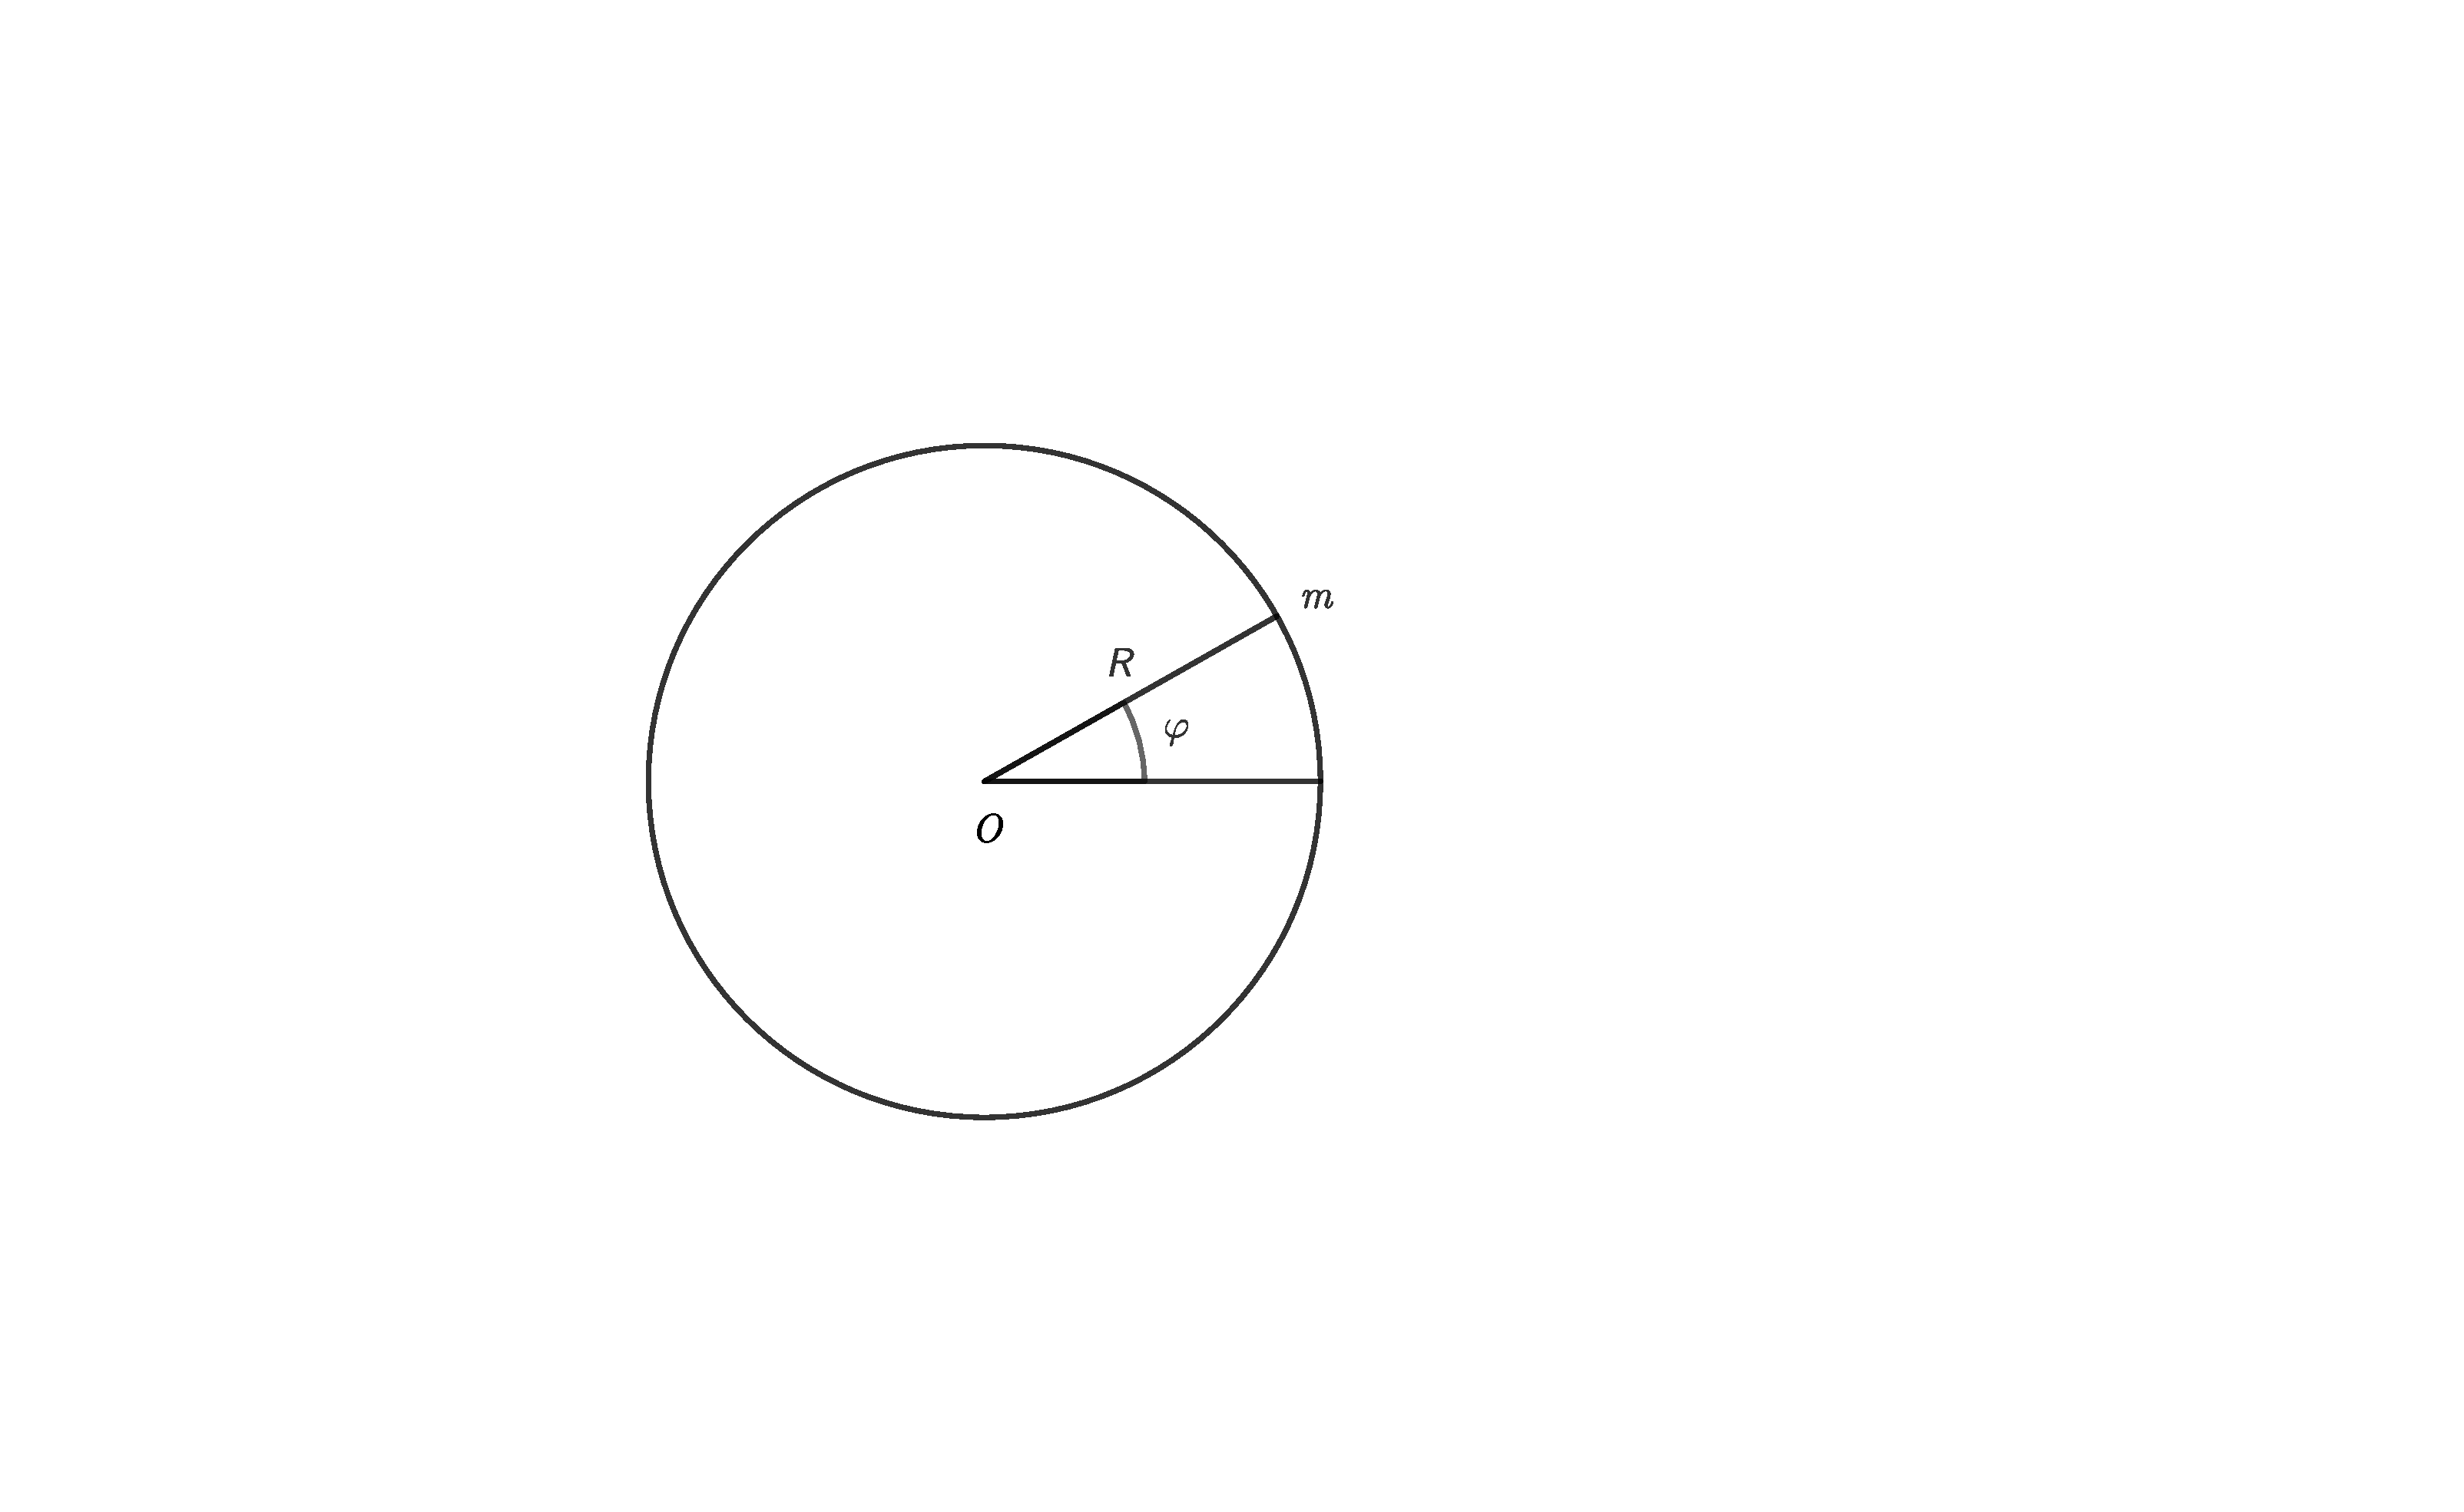
\includegraphics[width=2.5cm,clip]{QM file/figure/2-12}
	\caption{2-6题图}
	\label{fig.2-12}
\end{wrapfigure}

\exercise\label{ex2.6} 质量为$m$的粒子只能沿圆环(半径$R$)运动(如图\ref{fig.2-12}),能量算符为$\hat{H}=-\dfrac{\hbar^{2}}{2mR^{2}}\dfrac{d^{2}}{d\varphi^{2}}$,$\varphi$为旋转角.求能级($E_{n}$)及归一化函数$\varPsi_{n}(\varphi)$.讨论各能级的简并度.

本题是一种“平面转子”模型.平面转子的能量算符为
\begin{empheq}{equation*}
	\hat{H}=\frac{\hat{L}_{z}^{2}}{2I}=-\frac{\hbar^{2}}{2I}\frac{d^{2}}{d\varphi^{2}}
\end{empheq}
(在$x-y$面上旋转,转轴为$z$轴)其中$I$为转动惯量.

\exercise 对于一维运动,分布宽度$\Delta x$定义为
\begin{empheq}{equation*}
	\Delta x=(\bar{x^{2}}-\bar{x}^{2})^{\frac{1}{2}}
\end{empheq}
试对$\S$\ref{sec:02.04}中(1.)所讲的以及2-5题所求得的无限深势阱中的束缚态$\varPsi_{n}$,计算分布宽度$\Delta x$,并和经典力学的结论比较.
	
\begin{wrapfigure}[3]{r}{10em}
	\centering
	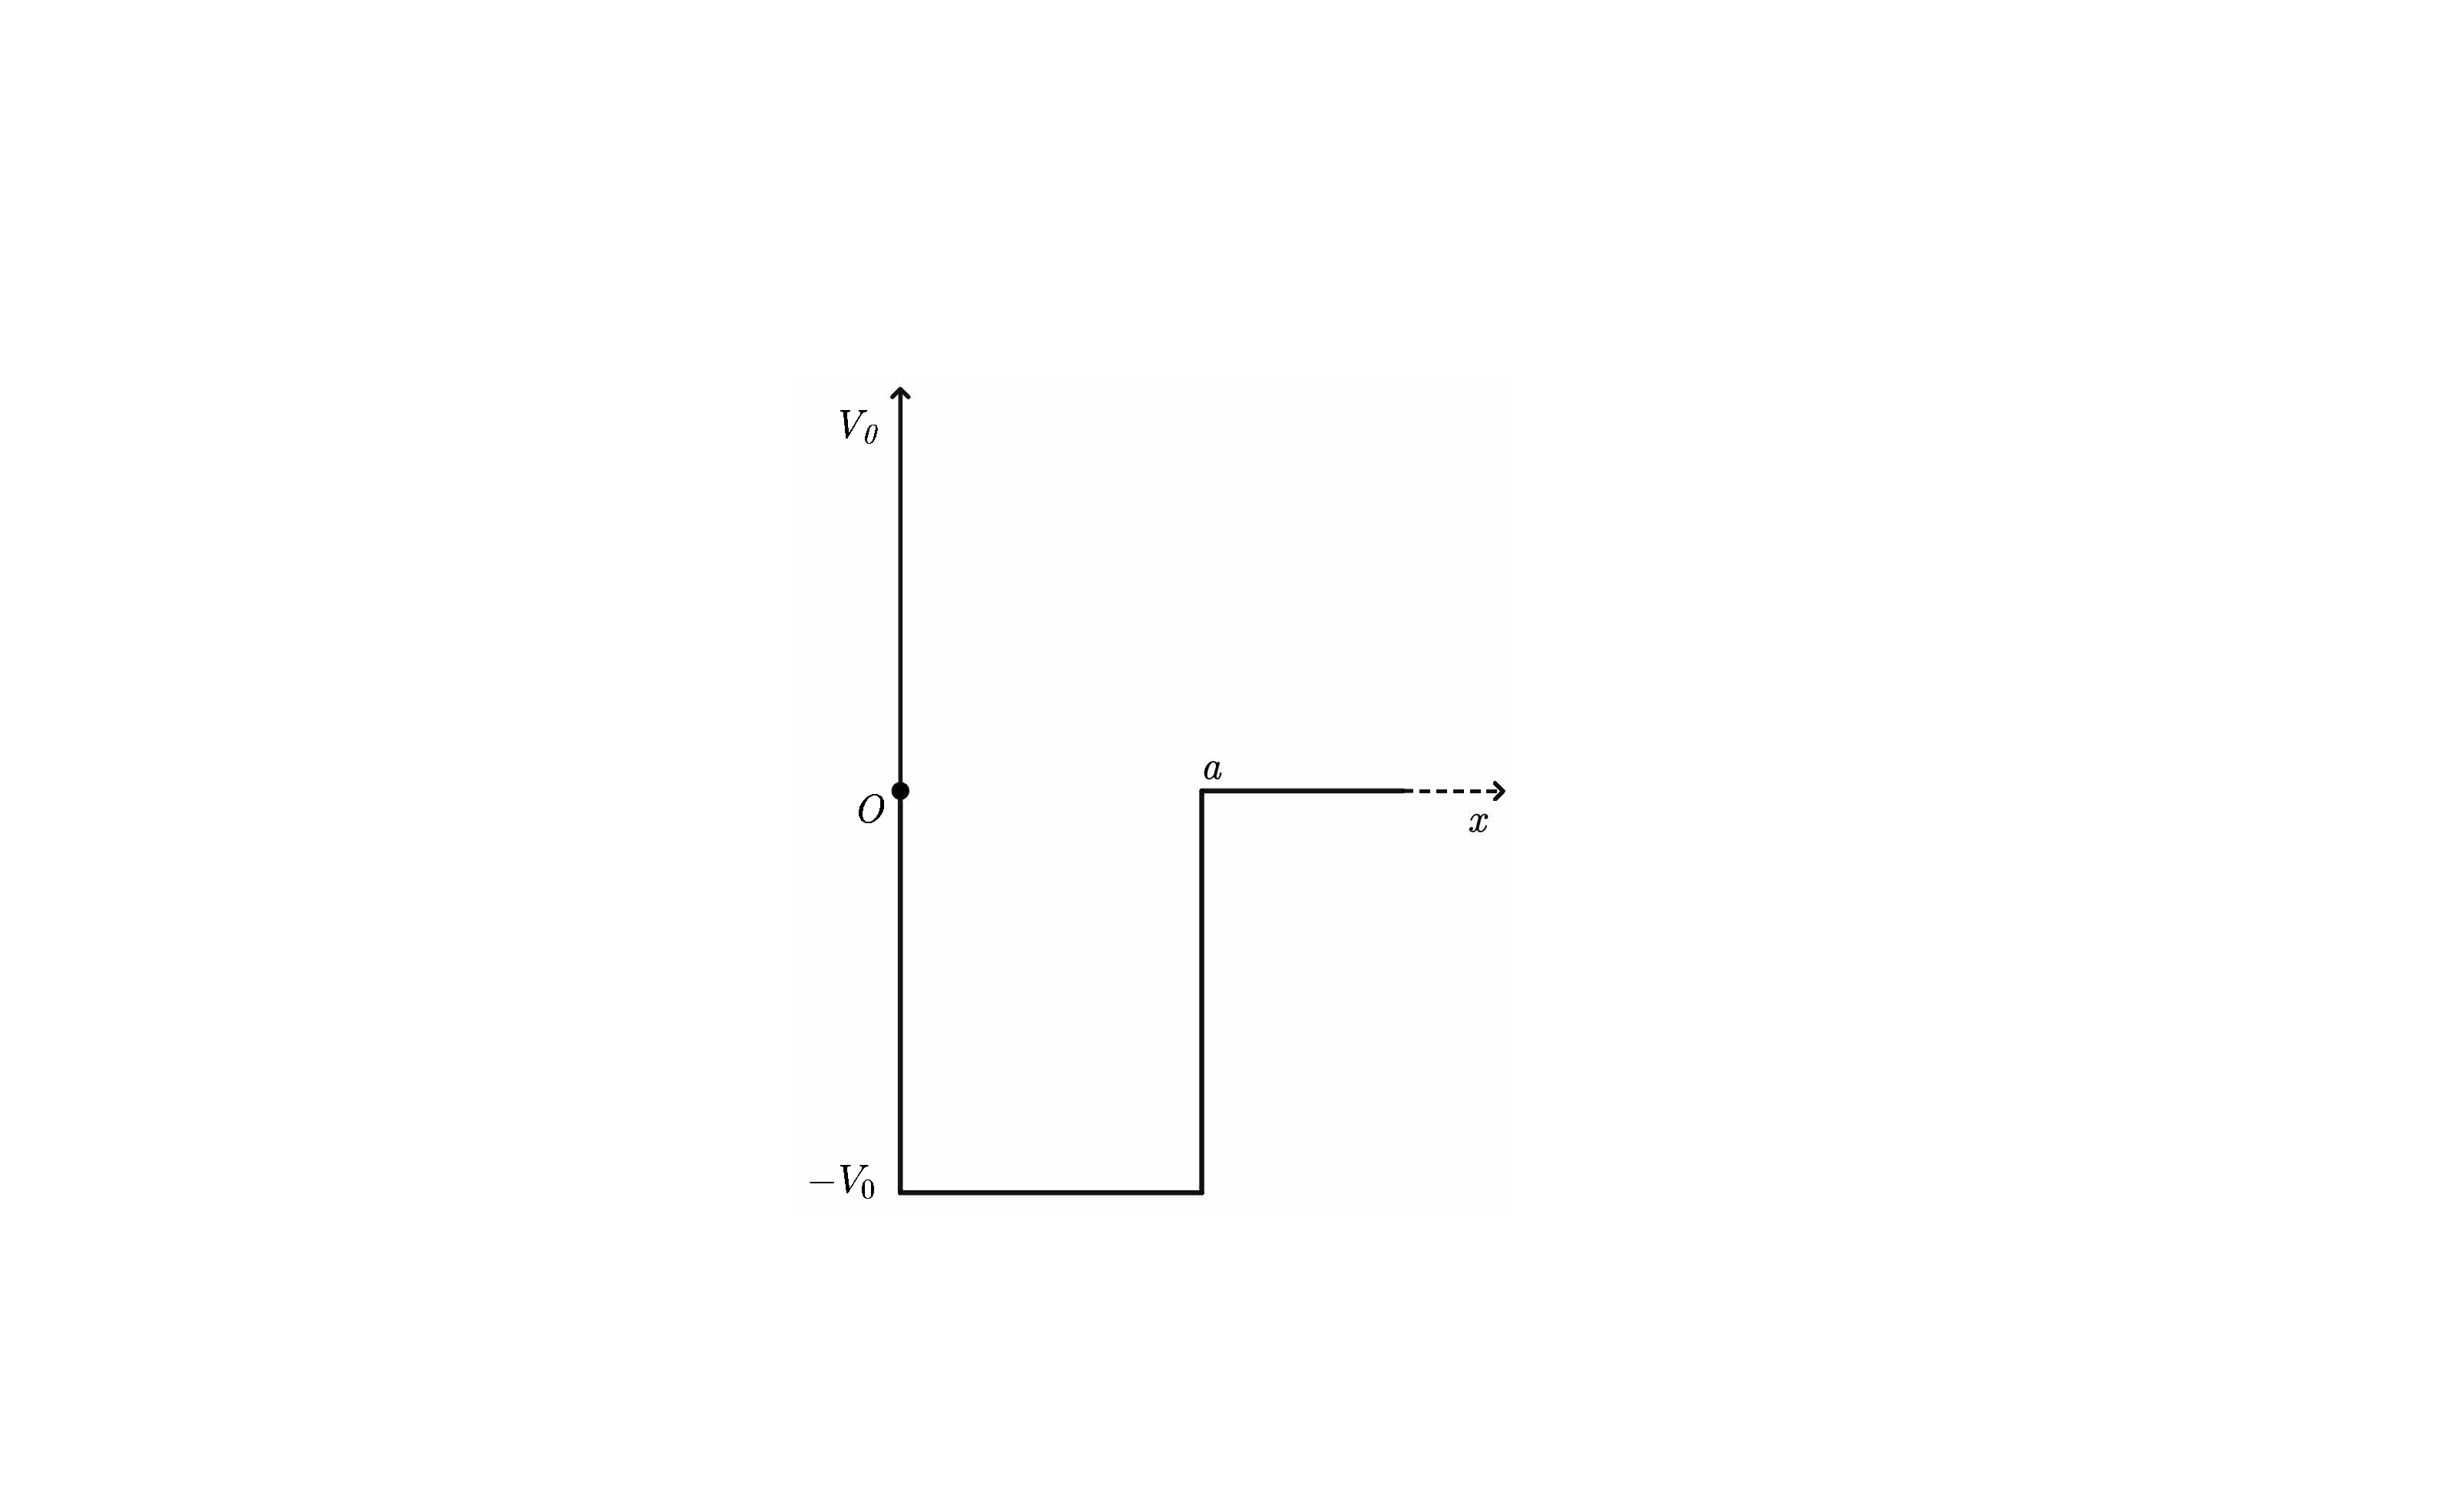
\includegraphics[width=3cm,clip]{QM file/figure/2-13}
	\caption{2-9题图}
	\label{fig.2-13}
\end{wrapfigure}
	
\exercise 对于$\delta$势阱造成的束缚态,计算$\bar{T},\bar{V},\Delta x,\Delta \boldsymbol{p}$.(定义见2-14题.)
	
\exercise 粒子在下列势阱中运动,
\setlength{\mathindent}{4em}
\begin{empheq}{equation*}
	V(x)=
	\begin{dcases}\notag
		\infty,	& x\geqslant 0	\\
		-V_{0}, & 0<x<a	\\
		0,		& x\leqslant a
	\end{dcases}
\end{empheq}\eqnormal
试证明仅当阱深、阱宽满足条件:
\setlength{\mathindent}{6em}
\begin{empheq}{equation*}
	V_{0}a^{2}>\frac{\hbar^{2}\pi^{2}}{8m}
\end{empheq}\eqnormal
时,才能存在束缚态($E<0$).并求能级方程.
	\pskip
\exercise 对于$\S$\ref{sec:02.04}中(2.)所讲有限深平底势阱,求

	(a)阱口刚好出现一个束缚态能级($E\approx0$)的条件.
	
	(b)束缚态能级总数,并和无限深势阱作比较.
	\pskip
\exercise 对于有限深平底势阱的第$n$个束缚态$\varPsi_{n}$,$E_{n}$,设$V_{0}\leqslant E_{n}+V_{0}$,计算

(a)粒子在阱外出现概率.

(b)$V(x)$和$V^{2}(x)$的平均值,并与$E_{n}$比较.
	\pskip
\exercise 对于谐振子的基态($\varPsi_{0}$)与第一激发态($\varPsi_{1}$),计算

(a)分布宽度$\Delta x$(定义见2-7题).

(b)粒子出现在经典禁区的概率.
	\pskip
\exercise 对于谐振子的能量本征态,证明下列公式
\begin{empheq}{equation*}
x\varPsi_{n}=\frac{x_{0}}{2}(\sqrt{n}\varPsi_{n-1}+\sqrt{n+1}\varPsi_{n+1})
\end{empheq}
\begin{empheq}{equation*}
	\frac{d}{dx}\varPsi_{n}=\frac{1}{\sqrt{2}x_{0}}(\sqrt{n}\varPsi_{n-1}-\sqrt{n+1}\varPsi_{n+1})
\end{empheq}

\exercise 利用上题中公式,求$\varPsi_{n}$的$\bar{T},\bar{V},\Delta x,\Delta \boldsymbol{p}$.$\Delta \boldsymbol{p}$定义为
\begin{empheq}{equation*}
	\Delta \boldsymbol{p}=(\bar{p_{x}^{2}}-\bar{p}_{x}^{2})^{\frac{1}{2}}
\end{empheq}

\exercise 二维各向同性谐振子,$\hat{H}=-\dfrac{\hbar^{2}}{2m}\bigg(\dfrac{\partial^{2}}{\partial x^{2}}+\dfrac{\partial^{2}}{\partial y^{2}}\bigg)+\dfrac{k}{2}(x^{2}+y^{2})$,试用分离变量法求能级和定态波函数,并求各能级的简并度.
	\pskip
\exercise 三维各向同性谐振子,$\hat{H}=-\dfrac{\hbar^{2}}{2m}\nabla^{2}+\dfrac{k}{2}(x^{2}+y^{2}+z^{2})$,试用分离变量法求能级和定态波函数,并讨论各能级的简并度.
	\pskip
\exercise 粒子在下列“切割谐振子势阱”中运动,
\begin{empheq}{equation*}
	V(x)=
	\begin{dcases}\notag
		\infty,				& x\geqslant 0	\\
		\frac{kx^{2}}{2},	& x>0
	\end{dcases}
\end{empheq}

求能级和定态波函数.

[提示:利用谐振子的结果.]

	\pskip
\exercise 二维耦合谐振子的能量算符为
\setlength{\mathindent}{5em}
\begin{empheq}{equation*}
	\hat{H}=\hat{T}+V=-\frac{\hbar^{2}}{2m}\bigg(\frac{\partial^{2}}{\partial x^{2}}+\frac{1}{2}m\omega^{2}(x^{2}+y^{2}\bigg)+\lambda xy
\end{empheq}\eqnormal

其中$|\lambda|<m\omega^{2}$.求能级.

[提示:作坐标变换$X=\dfrac{1}{\sqrt{2}}(x+y)$,$Y=\dfrac{1}{\sqrt{2}}(x-y)$容易证明:$\dfrac{\partial^{2}}{\partial x^{2}}+\dfrac{\partial^{2}}{\partial y^{2}}=\dfrac{\partial^{2}}{\partial X^{2}}+\dfrac{\partial^{2}}{\partial Y^{2}}$]

\newpage

\begin{wrapfigure}[9]{r}{10em}
	\centering
	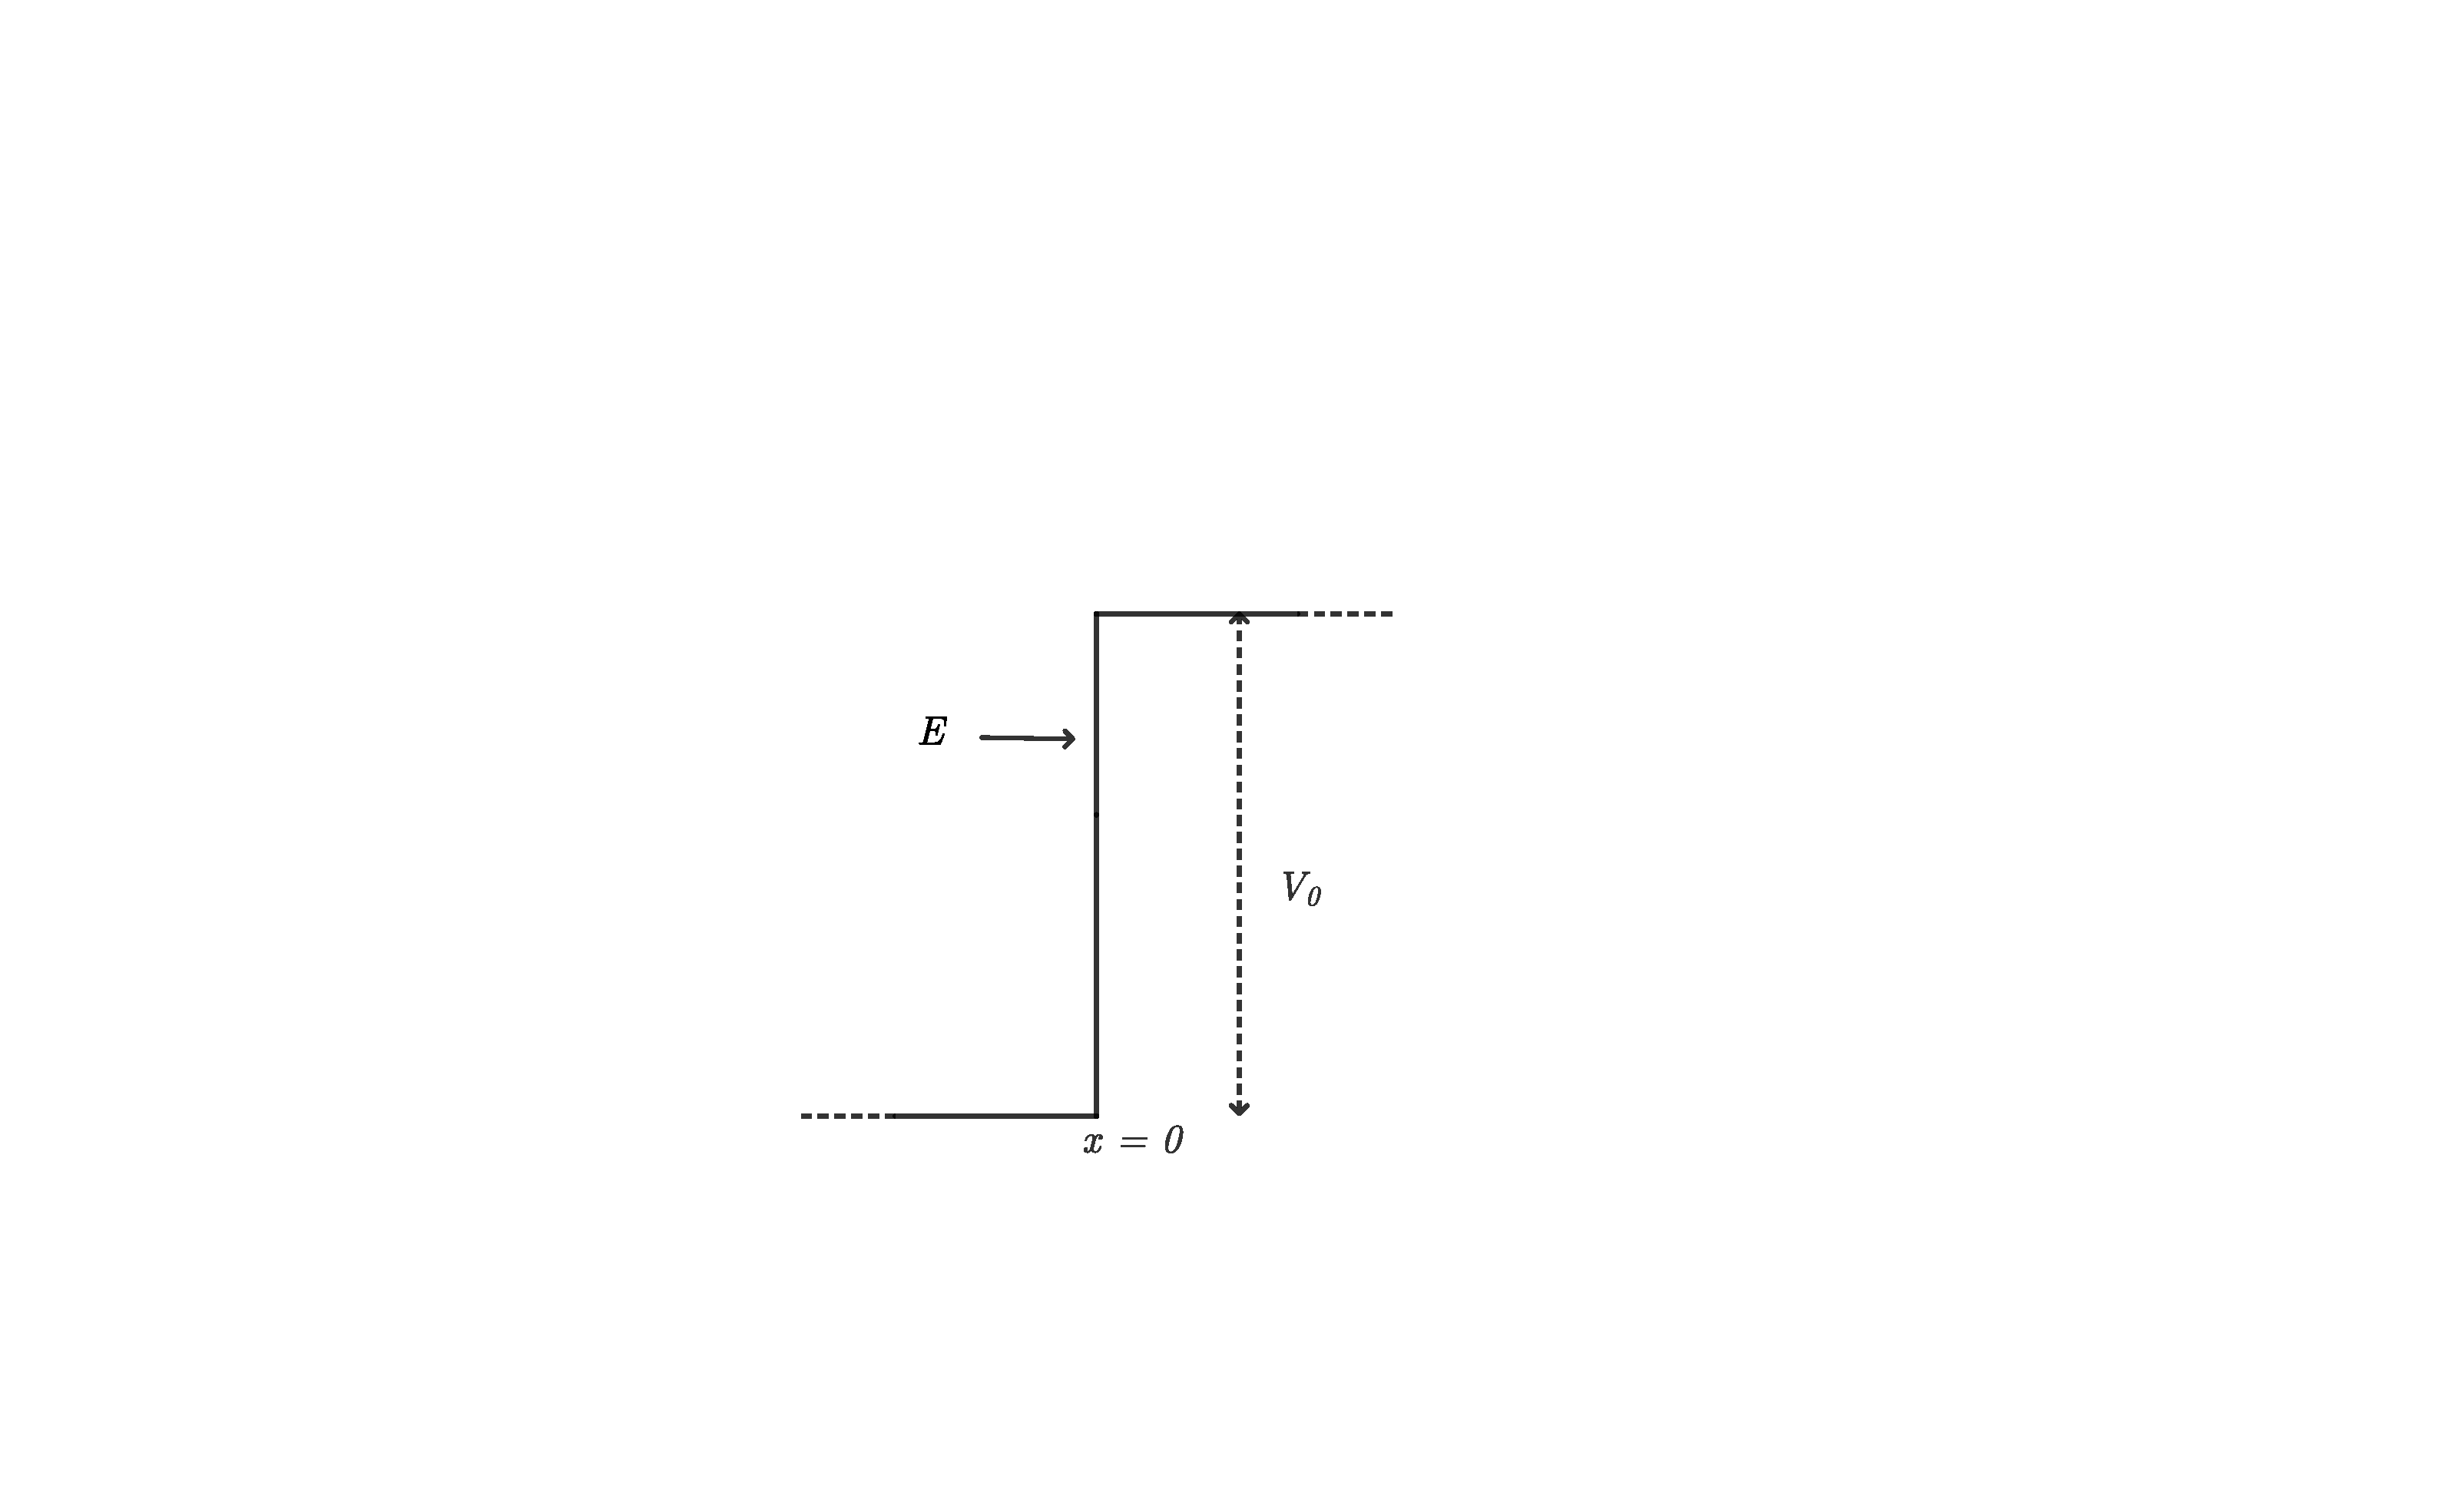
\includegraphics[width=3cm,clip]{QM file/figure/2-14}
	\caption{2-19题图}
	\label{fig.2-14}
\end{wrapfigure}
\exercise 粒子以动能$E=\dfrac{\hbar^{2}k^{2}}{2m}$从左方入射,遇势场(图\ref{fig.2-14})
\begin{empheq}{equation*}
	V(x)=
	\begin{dcases}\notag
		0,		& x<0	\\
		V_{0},	& x>0
	\end{dcases}
\end{empheq}

求反射系数和透射系数.($E>V_{0}$及$E<V_{0}$分别讨论.)
	\pskip
	\pskip
\exercise 粒子以动能$E=\dfrac{\hbar^{2}k^{2}}{2m}$从左方入射,遇$\delta$势垒$V(x)=\gamma\delta(x)$,$\gamma>0$,求透射系数.
\end{exercises}
